%fase de los filtros, linealidad
%estructura de los filtros (estructura z) (tipo de coef)
%consecuencias de fir e iir

%vistas - pantallazos

%%\textregistered
%%\texttrademark
%%\copyright


%% Pentiente
%diseño conceptual y marco teorico (2)(2)L
%Análisis de resultados (1)L
%introduccion (1)
%resumen (1)
%Metodologia (1)L
%Problema y justificación (1)L
%estado del arte ()
%conclusiones (1)

% 16 bits!!!
%%resultados () tiempos de grabación
%%trabajo futuro ()
%software%    poo (1)
%(imagenes matriz)
%Curva S
%Aspectos legales (imagenes y trademarks)
%apendices

% computational complexity
% - fft NlogN
% - for nivel: dwt N, logN
% - for nivel: idwt N

%% Nomenclaturas pendientes



% --------------------------------------------------------------------------- %
% Autor: William S\'anchez
% Materia: Anteproyecto, Proyecto de Grado
% Título: Propuesta proyecto de grado
% Propuesta: Dispositivo de análisis de señales de audio por medio de la transformada wavelet con aplicación en reconocimiento de emociones.
% Porofesor: Olga Lucia Quintero
% Julio/2013
% --------------------------------------------------------------------------- %
\documentclass[11pt,lettersize]{article} % Documento tipo artculo con tamao de letra a 12puntos (Obligatorio)
%\usepackage[latin1]{inputenc}
\usepackage[utf8]{inputenc}
\usepackage[spanish]{babel} %Idioma espa\~nol para los encabezados automaticos
%\usepackage[fixlanguage]{babelbib}
\usepackage[T1]{fontenc} %Fuentes para alfabeto espa\~nol (reconoce tildes, dieresis, e\~ne, las comillas, admiracion e interrogacion se ponen sin comandos especiales)

%%%%%%%%%%%%%%%%%%%%%%%%%%%%%%%%%%%%%%%%%%%%%%%%%%%%%%%%%%%%%%
%\documentclass[spanish,letterpaper,12pt,oneside,openany]{book}
%\usepackage[spanish]{babel}
\usepackage{babelbib}
\usepackage{etoolbox}
\patchcmd\btxselectlanguage{\csname}{\csname TEMPPATCH}{}{} % Para hacer a babelbib funcionar
%\usepackage{natbib}
\usepackage[margin=20pt,font=small,labelfont=bf,labelsep=period,justification=centerlast]{caption}%%Para modificar el formato del texto de los "caption"
%%%%%%%%%%%%%%%%%%%%%%%%%%%%%%%%%%%%%%%%%%%%%%%%%%%%%%%%%%%%%%

%\usepackage[top=3cm,bottom=3cm,left=4cm,right=2cm]{geometry} %Geometría del texto, normal
\usepackage[top=3cm,bottom=3cm,left=3cm,right=3cm]{geometry} %Geometría del texto, ambas caras
\pagestyle{plain} % Estilo de pagina sencillo. Numera en el centro inferior
\renewcommand{\baselinestretch}{1.4}  % Redefine el interlineado dinámico

\usepackage[mathcal,mathscr]{euscript} % Simbolos y fuentes matematicas
\usepackage{amscd,amsfonts,amsmath,amssymb,amsthm,amstext} % Simbolos y fuentes matematicas
%%
\usepackage{titlesec}  %% Modifica estilo de section y subsection
\titleformat*{\section}{\centering\normalfont\LARGE\bfseries}
\titlespacing{\section}{0pt}{*1}{*6}
%\titlespacing*{\section}{aftersep}[5cm]
\titleformat*{\subsection}{\normalfont\Large\bfseries}
%%
\usepackage{nomencl}
%\usepackage[intoc]{nomencl} %% Para agregar una tabla de nomenclaturas y abrebiaciones, [intoc] para agregarlo a la tabla de contenido
%% Ejemplo: \nomenclature{$a$}{The number of angels per unit area}
\usepackage{enumerate} % Ambiente para enumeracion de items
\usepackage{enumitem} % Para disminuir el interlineado en las listas con [nolistsep]
\usepackage{multicol} % Permite utilizar muticols para varias columnas en las listas
\usepackage{multirow} % Permite utilizar mutirows para varias filas en las listas
\usepackage[table]{xcolor} % Colores de tablas
\usepackage{array}
\usepackage{graphicx} % Para ambiente grafico
%\usepackage{subfigure}
%\includegraphics[trim = 10mm 80mm 20mm 5mm, clip, width=0.5\textwithd]{imagen} %% Para cortar un gráfico
\usepackage{float} % Para las tablas, permite usar H
%\usepackage{tabularx} % Para ambiente de listas y tablas

%%\usepackage{url} % Da formato a los hiperenlaces
%%\usepackage{hyperref}
%%\hypersetup{colorlinks=false}
%%\usepackage[hidelinks]{hyperref}
%%\usepackage[all]{hypcap}

%%%%%%%%%%%%%%%%%%%%%%%%%%%%%%%%%%%%%%%%%%%%%%%%%%%%%%%%%%%%%%
%%Dispositivo de análisis de señales de audio por medio de la transformada wavelet orientado al reconocimiento de emociones
%\usepackage[pdftex,pdfpagemode=UseOutlines,bookmarks,bookmarksopen,pdfstartview=FitH,colorlinks,linkcolor=blue, urlcolor=black, citecolor=blue]{hyperref} %%Para incluir detalles cucas del pdf
\usepackage[pdftex, pdftitle={Dispositivo de Analisis Wavelet}, pdfauthor={W. Sanchez}, pdfsubject={Tesis de Pregrado}, pdfkeywords={Analisis de señales, Transformada Wavelet, Análisis multiresolución, Reconocimiento de Emociones, Raspberry Pi}, pdfpagemode=UseOutlines,bookmarks,bookmarksopen,pdfstartview=FitH,colorlinks,linkcolor=blue, urlcolor=black, citecolor=blue]{hyperref} %%Para incluir detalles cucas del pdf

%%\url{<my_url>} %% Escribe URL 
%%\href{<my_url>}{<text>} %% Escribe <text> y lo vincula a la URL 
%%\hyperref[<label_name>]{<link text>} %% Vincula el <link text> al <label_name>
%%\hyperref[<label_name>]{<title> \ref*{<label>}} %% Extiende el vinculo de \ref* ha <title>, \ref* nombre no vinculo
%%\hypertarget{label}{target caption} %% Genera un target
%%\hyperlink{label}{link caption} %% Genera un vinculo al target

%\usepackage[draft]{pdfpages}%%Para incluir archivos en pdf
\usepackage[final]{pdfpages}%%Para incluir archivos en pdf
\usepackage{cite}  %% Para poner bonitas las citas
\usepackage{bookmark} %% Para poder organizar las etiquetas en pdf
%Ejemplo: \pdfbookmark[0]{Tabla de contenido}{} % en la tabla de contenido
%%%%%%%%%%%%%%%%%%%%%%%%%%%%%%%%%%%%%%%%%%%%%%%%%%%%%%%%%%%%%%

\usepackage[none]{hyphenat} % NO más separación de palabras
\sloppy % Disminuye la separacion de palabras a final de renglón y mejora el justificado
%\hyphenation{si-la-bas}
\frenchspacing \setlength{\parindent}{0mm} % Controla la sangria del primer renglon de un parrafo

%% Redefinir los encabezados automáticos
\addto\captionsspanish{
\renewcommand{\contentsname}{Tabla de contenido}
\renewcommand{\figurename}{Figura}
\renewcommand{\listfigurename}{Lista de figuras}
\renewcommand{\tablename}{Tabla}
\renewcommand{\listtablename}{Lista de tablas}
\renewcommand{\nomname}{Lista de abreviaturas y símbolos}
\renewcommand{\abstractname}{Resumen}
\renewcommand{\refname}{Referencias}
}
%\abstractname 	Resumen
%\alsoname 	    ver también (paquete makeidx)
%\appendixname 	Apéndice
%\bibname 	    Bibliografía (report,book)
%\ccname 	    cc (letter)
%\chaptername 	Capítulo (report,book)
%\contentsname 	Íncide
%\enclname 	    encl (letter)
%\figurename 	Figura (para flotantes)
%\headtoname 	a (letter)
%\indexname     	Index
%\listfigurename 	Lista de Figuras
%\listtablename 	Lista de Tablas
%\pagename 		Página (letter)
%\partname 		Parte
%\refname 		Referencias (article)
%\seename 		ver (paquete makeidx)
%\tablename 		Tabla (para flotantes)

%% Commands
%\DeclareMathOperator{\e0}{\epsilon_{0}} % Declaracion de operador matematico
%\DeclareMathOperator{\m0}{\mu_{0}} % Declaracion de operador matematico
%\newcommand{\uni}[1]{\left[ {#1}\right] }
%\newcommand{\unif}[2]{\left[ \frac{#1}{#2}\right] }

%\newcommand{\dis}[1]{$\displaystyle{#1}$} % Definicion de un comando por usuario. Estilo matematico para incorporar en texto
%\DeclareMathOperator{\sen}{sen} % Declaracion de operador matematico
%\newcommand{\ket}[1]{|{#1}\rangle}
%\newcommand{\bra}[1]{\langle{#1}|}
%\newcommand{\ketbra}[2]{|{#1}\rangle\langle{#2}|}
%\newcommand{\braket}[2]{\langle{#1}|{#2}\rangle}
%\newcommand{\braxket}[3]{\langle{#1}|{#2}|{#3}\rangle}
%\newcommand{\etime}[1]{e^{-i{#1}t/\hbar}}
\newcommand{\tabla}[1]{\hyperref[{#1}]{tabla \ref*{#1}}}
\newcommand{\figura}[1]{\hyperref[{#1}]{figura \ref*{#1}}}
\newcommand{\seccion}[1]{\hyperref[{#1}]{sección \ref*{#1}}}
\newcommand{\ecuacion}[1]{\hyperref[{#1}]{ecuación \ref*{#1}}}

%\theoremstyle{definition}
%\newtheorem{defin}{Definición}[section]

\makenomenclature  %% Comienza la nomenclatura
\begin{document} %Inicio del documento (Obligatorio)

%------------------------- Contenido ---------------------------------%
%Portada
%Página de aceptación
%Página de dedicatoria
%Página de agradecimientos
%Tabla de contenido.
%Listas especiales
%
%Resumen, Palabras claves
%
%Introduccion (contexto)
%Esta es obligatoria. En ella el autor presenta el documento, explica porque es importante, cuáles son los antecedentes del trabajo, los objetivos, el alcance, la metodología empleada y la aplicación en el área del conocimiento
%
%Estado del arte
%- Analisis de señales de audio (Wavelet)
%- Dispositivos y software de analisis de señales
%- .Tecnicas reconocimiento de emociones
%- .Dispositivos y software de ER
%
%Revisión teórica
%- Conversión ADC
%- Transformada de fourier ??
%- Transformada wavelet (Efficient Implementations of Discrete Wavelet Transforms Using FPGAs)
%- Complejidad algoritmica ??
%- Algoritmo (Seudocódigo) ??
%- voz humana y emociones
%- Filtros
%
%Revisión de hardware
% Diseño conceptual
% - Estructura (~Planteamiento del problema)
% - Requerimientos
% - Valoración de requerimientos (1-5)
% - Matriz morfológica
% - Ruta
%- Micrófonos
%- ADC click (SPI)
%- Audio USB
%- Raspberry Pi
%
%Revisión de software
%- Rasbian
%- alsa
%- Python (g++)
%- scipy.io.wavfile (varias maneras de hacerlo)
%- numpy.fft
%- pywt (scipy.signal sunpy)
%- tkinter (Qt...)
%
%Implementacion
%
%Resultado
%
%Conclusiones
%- Adc click muy lento bajo esta aplicacion, maximo de 5k-8k
%- Utilidad y futuro de Audio-USB (osciloscopio)
%- Muy buen futuro para el analisis de emociones
%- Wavelet validadas, ende analisis es bueno
%- Cambiar los tiempos para que den cantidades de datos multiplos de 2
%- 
%- 
%- ES BUENO O NO EL RESULTADO?
% Trabajo futuro
%- Reconocimiento de emociones
%- Modo de tiempo real:
%   - Un core mas veloz (Rpi)
%   - Interfaz grafica independiente
%   - Aplicacion sin graficas
%   - Lenguaje más rápido (copilado) [c++ tiene librerias WT]
%
%
% Diseño conceptual del dispositivo, partiendo de la identificación de los requerimientos técnicos y del usuario.
% Diseñar las etapas de adquisición, pre-procesamiento y procesamiento de la señal de audio.
%%\ Diseñar y desarrollar el algoritmo de análisis de la señal.
% Construir la planta física y verificar la correcta comunicación entre los periféricos utilizados.
% Digitalizar la señal de audio por medio del convertidor analógico digital escogido en el diseño conceptual, teniendo en cuenta el análisis espectral de la señal fenomenológica aplicando conceptos básicos de muestreo y retención de datos.
% Desarrollar los algoritmos de pre-procesamiento y procesamiento de la señal.
%%\ Implementar filtros para la señal adquirida.
%Implementar los algoritmos desarrollados.
%Realizar pruebas del dispositivo piloto final para evaluar su desempeño, por medio de la comparación con herramientas de programación ya validadas o datos reportados en la literatura.
%
%
%Bibliografía
%Las citas bibliográficas se organizan alfabéticamente, según el apellido del autor o de los títulos cuando la obra es anónima o se desconoce el autor. (IBID[IBID, pag], Op. Cit.[apellido, Op. Cit, pag])
%
%Bibliografía complementaria
%Es el listado de documentos que se relacionan con el tema, pero que no fueron consultados para la elaboración del trabajo y pueden servir como fuentes de información para ampliar el tema. Se organiza de la misma forma que la bibliografía principa
%


%Notas:
%Los títulos de los capítulos se escriben dejando un margen superior de 3 centímetros al comienzo de la hoja, con mayúscula sostenida, centrados y sin punto final, y se separan del texto con doble espacio. 
%Los títulos de segundo nivel se escriben igual que los títulos de primer nivel pero se alinean a la izquierda. 
%Los títulos de tercer nivel se escriben en mayúscula inicial y punto seguido, el texto debe continuar en el mismo renglón.

%Titulo de la propuesta.
%Asesor principal.
%Planteamiento del problema. (Estado del arte 2p)
%Objetivos de la propuesta.
%Justificación de la propuesta. (Interés de resolverlo, trabajo de grado IF(Áreas de la física))
%Metodología (Resursos)
%Cronograma de actividades.
%Presupuesto.
%Productos
%Bibliografía.

%\frontmatter
%------------------------- Portada -----------------------------------%
%\pdfbookmark[1]{Portada}{}
\pagenumbering{Roman}
\thispagestyle{empty} % Esta pagina no se numera
\begin{center}
\textbf{\\[1.5cm]{\LARGE Dispositivo de análisis de señales de audio por medio de la transformada wavelet orientado al reconocimiento de emociones}}\\[5cm]
{\Large William Fernando S\'anchez} \\ {\large \textit{wsanche2@eafit.edu.co}}\\[7.5cm]
Ingenier\'ia F\'isica \\ Departamento de Ciencias Básicas \\ Escuela de Ciencias y Humanidades \\ Universidad EAFIT \\ Medell\'in, Colombia.\\
%wsanche2@eafit.edu.co \\ [.1cm]
2013
\end{center}
\pagebreak

%------------------------- Portada 2----------------------------------%
\thispagestyle{empty} % Esta pagina no se numera
\begin{center}
\textbf{{\Large Dispositivo de análisis de señales de audio por medio de la transformada wavelet orientado al reconocimiento de emociones}}\\[3cm]
{\Large William Fernando S\'anchez} \\ {\large \textit{wsanche2@eafit.edu.co}}\\[2.5cm]
{\large\emph{\textbf{Trabajo de grado presentado como requisito }}\\
\emph{\textbf{parcial  para optar al t\'itulo de Ingeniero Físico}}}\\[3cm]
%{\large \textbf{Tesis} \\ \textbf{Proyecto de grado}}\\[2cm]
{\large \textbf{Asesora:} \\ Doctora Olga Lucía Quintero}\\[3cm]
Ingenier\'ia F\'isica \\ Departamento de Ciencias Básicas \\ Escuela de Ciencias y Humanidades \\ Universidad EAFIT \\ Medell\'in, Colombia.\\
%wsanche2@eafit.edu.co \\ [.1cm]
2013
\end{center}
\pagebreak

% Dispositivo piloto para análisis de sonido por medio de la transformada wavelet con aplicación en vocalizaciones afectivas
% Dispositivo piloto para el análisis de sonido por medio de transformada wavelet con aplicación en reconocimiento de emociones
% Dispositivo piloto para análisis de señales de audio por medio de la transformada wavelet
% Prototipo de análisis de señales de audio por medio de la transformada wavelet con aplicación en reconocimiento de emociones
% Prototipo de análisis de señales de audio por medio de la transformada wavelet
% Dispositivo de análisis de señales de audio por medio de la transformada wavelet con aplicación en reconocimiento de emociones

%------------------------- Aceptación --------------------------------%
%%%Nota de aceptacion
\begin{flushright}
	Nota de aceptaci\'on\\
	\vspace{1cm}
	\rule{\textwidth}{1pt}\\
	\vspace{1cm}
	\rule{\textwidth}{1pt}\\
	\vspace{1cm}
	\rule{\textwidth}{1pt}\\
	\vspace{1.3cm}
	Presidente del jurado\\
	\vspace{1cm}
	\rule{\textwidth}{1pt}\\
	\vspace{1.3cm}
	Jurado\\
	\vspace{1cm}
	\rule{\textwidth}{1pt}\\
	\vspace{1.3cm}
	Jurado\\
	\vspace{1cm}
	\rule{\textwidth}{1pt}\\
	\vspace{2.5cm}
	\rule{\textwidth}{1pt}\\
	\vspace{.8cm}
	Ciudad y Fecha
\end{flushright}
\thispagestyle{empty}
\pagebreak

%------------------------ Dedicatoria --------------------------------%
%\vspace*{5cm}
%\begin{flushright}
%\begin{tabular}{p{10cm}r}
%\emph{``FRASE''} \\
%\textbf{AUTOR}
%\end{tabular}
%\end{flushright}
%\thispagestyle{empty}

%---------------------- Agradecimientos ------------------------------%

%\section*{Agradecimientos}
%Quiero agradecer inicialmente a mi familia por apoyarme en el desarrollo de la Maestr\'ia as\'i como el presente documento, particularmente a mis padres a quienes admiro --aunque no suela decirlo a menudo.
%
%Tambi\'en debo mi gratitud al Profesor Juan David G\'omez quien fue mi asesor durante el desarrollo del trabajo que ac\'a est\'a condensado. Como asesor permiti\'o que yo afianzara mis conocimientos en la propagaci\'on de ondas y la f\'isica computacional, para mi placer, temas que ac\'a se presentan aunados. Al Profesor Mario Elkin V\'elez quien siempre ha tenido su puerta abierta para discusiones sobre gran diversidad temas, muchos de ellos relacionados con el tratamiento formal de los fen\'omenos f\'isicos presentados. Al Profesor Juan Diego Jaramillo por su \'enfasis en el comportamiento f\'isico sobre los \emph{hechos} matem\'aticos relacionados con la propagaci\'on de ondas y las vibraciones en estructuras.
%
%A la Profesora Anne Christine Hladky-Hennion del \emph{Institut d'\'electronique de micro\'electronique et de nanotechnologie -Universit\'e Lille Nord}, Francia. Por responder tan amablemente a mis consultas conceptuales relacionadas con la propagaci\'on de ondas mec\'anicas en materiales peri\'odicos y quien adem\'as me env\'io una copia impresa de la tesis de Philippe Langlet, que sirvi\'o como soporte para el desarrollo del trabajo.
%
%Gracias a Edward Villegas, Santiago Echeverri y Yhefferson Guti\'errez por la gran cantidad de discusiones relacionadas con los cristales electr\'onicos, fot\'onicos y fon\'onicos y las discusiones en f\'isica del estado s\'olido. Por las discusiones en general, no creo pr\'actico hacer menci\'on de las muchas que han habido. Especial agradecimiento a Yhefferson quien me permiti\'o hacer reproducci\'on de uno de los cap\'itulos de su trabajo de grado como anexo en este documento.
%
%Finalmente, quiero expresar mi gratidud con Colciencias y a la Universidad EAFIT por apoyarme en dos ocasiones como Joven Investigador en el Programa J\'ovenes Investigadores e Innovadores ``Virginia Guti\'errez de Pineda''.
%
%\thispagestyle{empty}

%---------------------- Tabla de contenido ---------------------------%
%\pdfbookmark[1]{Tabla de contenido}{}
\pdfbookmark[1]{\contentsname}{}
\tableofcontents
\cleardoublepage \phantomsection
%\newpage
\listoftables
\addcontentsline{toc}{section}{\protect\numberline{}\listtablename}
%\pdfbookmark[1]{Lista de tablas}{}
\cleardoublepage \phantomsection
%\newpage
%\listfigurename
\listoffigures
\addcontentsline{toc}{section}{\protect\numberline{}\listfigurename}
%\pdfbookmark[1]{Lista de figuras}{}
\cleardoublepage \phantomsection
%\newpage
\printnomenclature[2cm] %% Imprime la nomenclatura
\addcontentsline{toc}{section}{\protect\numberline{}\nomname}
%\pdfbookmark[1]{Lista de abreviaturas y símbolos}{}


%\mainmatter
%------------------- Resumen, Palabras claves ------------------------%
\cleardoublepage \phantomsection
\pagenumbering{arabic}
\section*{Resumen}
\addcontentsline{toc}{section}{\protect\numberline{}Resumen}
Este trabajo dirigido de grado busca la consolidación del proceso de apropiación del conocimiento del Ingeniero Físico, en coherencia con el objetivo del programa: ``formar profesionales con una excelente fundamentación en ciencias básicas, en donde la Física Aplicada es el hilo conductor en la formación científica, al lado de una formación en diversos tópicos fundamentales de la Ingeniería, que posibilitan la comprensión, apropiación y aplicación de los principios involucrados en la solución de muy diversos problemas reales asociados con el uso de nuevas tecnologías''.\\

El trabajo de grado se compone de la implementación en prototipo de hardware de un dispositivo que pueda adquirir, digitalizar, reprocesar, analizar y descomponer una señal de audio (onda mecánica) con el fin de hacer una aproximación a la aplicación de detección de cambios emocionales en el marco de la investigación en curso titulada “Sistema Automático de Detección de Cambios Emocionales en audio con propósitos de auditoría y control. Desarrollo de un prototipo”.\\

Para ello, el estudiante hizo uso de sus conocimientos para la aprehensión y entendimiento del fenómeno físico en cuestión, dentro del marco conceptual de la aplicación que lo requiere; y con esto, usar la matemática (teorías de análisis de Fourier, muestro, filtrado, control digital, análisis wavelet) para el cumplimiento completo de los objetivos del proyecto. Es decir, con el fundamento de la formación adquirida desde la física, la matemática, la electrónica, el control automático y el uso de la tecnología, este trabajo presenta la primera versión de un dispositivo que responde a las necesidades de la investigación.

%------------------- Introduccion (contexto) -------------------------%
\cleardoublepage
\phantomsection
\section*{Introducción}
\addcontentsline{toc}{section}{\protect\numberline{}Introducción}
Como se mencionó anteriormente, el prototipo desarrollado, responde a las necesidades de la investigación en detección de emociones en el que, los investigadores de los grupos de investigación Modelado Matemático, Análisis funcional y Aplicaciones y Grupo de I+D+I en Tecnologías de la Información y las Comunicaciones (GIDITIC) de la Universidad EAFIT, ofrecen el desarrollo de una herramienta tecnológica para aumentar el cubrimiento de las tareas realizadas por las áreas de auditoría y compliance de las mesas de negocio del Grupo Bancolombia.\\

Específicamente, el prototipo desarrollado, es una herramienta que permite agilizar y mejorar los procesos de detección de anomalías en las transacciones de las mesas de negocios, mediante el análisis de las señales de audio (voces de los involucrados en la negociación) de las mismas. Ésta consta de tres componentes: el primero es un sistema que permite evaluar, sobre las conversaciones sostenidas entre los traders y los clientes del banco, el uso de las palabras de un diccionario previamente definido por el área de compliance del banco; este componente usará una técnica de conversión de audio a texto y un proceso de minería de datos sobre el texto.\\

El segundo componente detecta los cambios en las emociones asociadas a las transacciones realizadas, mediante un análisis espectral en tiempo y frecuencia de las señales de audio usando transformadas waveletes (ondita-ondícula) y asociándolas con el plano valencia (de positiva a negativa) y excitación (de alta a baja). Finalmente, como tercer componente se plantea el uso de un sistema de inferencia que reproduzca el conocimiento de los auditores expertos, y que implemente herramientas de inteligencia artificial permitiendo fusionar los resultados entregados por los primeros dos componentes. Esto con el fin de reportar la posible presencia de comportamientos anormales durante la transacción.\\
%
En contraste con las soluciones que se ofrecen en la industria, este proyecto combina diferentes técnicas, en las cuales los investigadores de los tres grupos de investigación mencionados son expertos, proporcionando una herramienta a la medida de la problemática del Banco.\\

En adición, este proyecto fortalece los lazos entre la Universidad y el Banco mediante la vinculación de estudiantes de maestría y pregrado a la investigación propuesta y consolida la cocreación con la academia como una opción de ejecución de la estrategia de desarrollo tecnológico.\\

Finalmente, como pilar del aporte científico se destaca la creación de una línea de investigación interdisciplinar alrededor del estudio de las emociones mediante herramientas desde la ingeniería, la matemática, la psicología e incluso la filosofía. Se estimula el fortalecimiento de la capacidad investigativa de los grupos de investigación vinculados y la continuidad en la creación de nuevo conocimiento que pueda ser trasladado eventualmente a otras áreas de aplicación como por ejemplo la psicología del desarrollo infantil.\\

Desde el punto de vista tecnológico, se han presentado en el mercado diversas soluciones para el análisis de la voz a través de llamadas telefónicas. La mayoría de estas opciones están orientadas a su utilización en los call centers. Las características de algunas de las soluciones disponibles a nivel mundial, no se adaptan a los requerimientos que son de interés particular para su uso en pro de las necesidades del Banco.\\

En un ejercicio de exploración tecnológica realizado a nivel interno basado en fuentes como Gartner y Forrester, se concluyó que las compañías más importantes que ofrecen programas de Speech Analysis a nivel mundial son Nice y Verint. Estas brindan software bastante completos y que, si bien se emplean principalmente en call centers, pueden ser usadas en otro tipo de empresas. Algunas de ellas contienen incluso detección de emociones, separación de voces, transcripción audio-texto, análisis en tiempo real, indexación fonética, detección de interrupciones y análisis de problema entre el agente y el cliente. No obstante estas aplicaciones no se adaptan a los términos idiomáticos del país ni a la jerga de los traders, la cual incluye numerosos términos financieros técnicos, abreviaciones dada la agilidad con la que deben ser cerradas las operaciones y siglas en inglés y español.\\

Por otro lado, se realizó un segundo ejercicio de exploración tecnológica en donde se identificaron nuevos proveedores de soluciones para el análisis de la voz, concluyendo que las tecnologías empleadas para dicho fin son diversas y por ende no existen patrones que marquen una tendencia tecnológica clara en esta industria. \\

Estas herramientas, están disponibles a un alto costo, por lo que se hace importante y necesario el desarrollo de herramientas locales, desarrolladas con base en los requerimientos específicos de la Organización y apoyadas en el ecosistema académico, donde investigadores están en capacidad de proponer, desde sus áreas del conocimiento, soluciones eficaces al problema.\\

El reconocimiento automático de las emociones a partir de la voz, ha sido en la última década un área de estudio en la interacción humano-computador y procesamiento de señales de audio. Este tipo de enfoque se ha realizado principalmente con aplicaciones en sistemas de diálogo o call centers.\\

Hay algunos estudios sobre los problemas técnicos que surgen de la implementación de interfaces humano-computador con la habilidad de reconocer las emociones vocales del usuario \cite{Vogt2008}. Los trabajos relacionados se focalizan en las propiedades fonéticas y acústicas del lenguaje hablado afectivo. Los parámetros vocales que han sido más investigados en estudios psicológicos en relación con la emoción y que son además intuitivos son la prosodia (tono, intensidad y velocidad de habla) y la calidad de la voz. Murray y Arnott \cite{Murray1993} escribieron una revisión de la literatura en emociones a partir del habla y se refirieron a un número de estudios que también habían identificado correlaciones acústicas inequívocas de las emociones. Estos estudios muestran que la prosodia y la calidad de la voz son los rasgos más importantes para distinguir entre emociones de acuerdo a la percepción humana. En particular, el tono y la intensidad parecen estar correlacionadas con la activación, de modo que intensidad y tonos altos implican activación alta y un tono bajo e intensidad baja implican baja activación.\\

Sin embargo, estos estudios psicológicos se basan en un conjunto de datos de personas que simulan la emoción, y no la expresan de una manera real y espontánea. Este tipo de mapeos de variables acústicas pueden ser posibles en un número de casos, incluso actuados, dado que las variaciones intra e inter hablantes son tan altos como la expresividad de las emociones es dependiente de la personalidad o el humor.\\

Para los investigadores de este proyecto, este enfoque no resulta ser el mejor puesto que se plantea la extracción de las emociones a partir de una base de datos reales de las conversaciones de los traders de la mesa de negocios del banco. Se plantea de esta manera porque la propuesta no trata de realizar un ejercicio netamente para investigación psicológica, sino una herramienta tecnológica desarrollada a la medida de la empresa Bancolombia con la cual las emociones inducidas no son las que se desean identificar.\\

Según la literatura, en cada interacción computador hombre, las emociones que ocurren son espontáneas, usualmente presentadas en variaciones considerablemente altas en los parámetros que las caracterizan, además de no ser emociones prototípicas pero que pueden estar enmascaradas, mezcladas o débiles y difícilmente distinguibles. Esto hace la tarea de reconocimiento de emociones mucho más difícil, de modo que aún la mayoría de los rasgos acústicos necesitan ser investigados. Claro está, que el reconocimiento de las emociones realizado personalizadamente es lo más confiable \cite{Wilting2006}. \\

Sobre esta línea de pensamiento, la pregunta natural surge de la construcción de una buena base de datos. Para ello, la literatura señala que las bases de datos con frases emocionales o ``discursos emocionales'' no son sólo esenciales en este tipo de estudios psicológicos, sino que también lo son para el reconocimiento automático de emociones, dado que los métodos estándares son de naturaleza estadística y necesitan aprender con ejemplos.\\

Como fue mencionado anteriormente, en este proyecto se plantea la posibilidad de mapear los rasgos extraídos de las señales de audio al espacio emocional, el cual es un modelo bi-dimensional del afecto. Las dimensiones de este espacio, son usualmente valencia (de positiva a negativa) y excitación (de alta a baja) y algunas veces una tercera dimensión llamada postura (de abierta a cerrada). Este modelo es básicamente una representación en el plano, de la ubicación de las emociones más importantes en los seres humanos \cite{Russell1979},\cite{Russell1980},\cite{Russell1989},\cite{Russell1999}. El modelo dimensional permite una descripción continua que es coherente con las emociones espontáneas. Grimm et al \cite{Grimm2007} usaron una técnica de regresión para clasificar en un espacio continuo de tres dimensiones. En la \figura{F-dimensions-emotion} se muestra un ejemplo de la representación en 2 dimensiones.

\begin{figure}[h!]
	\centering
	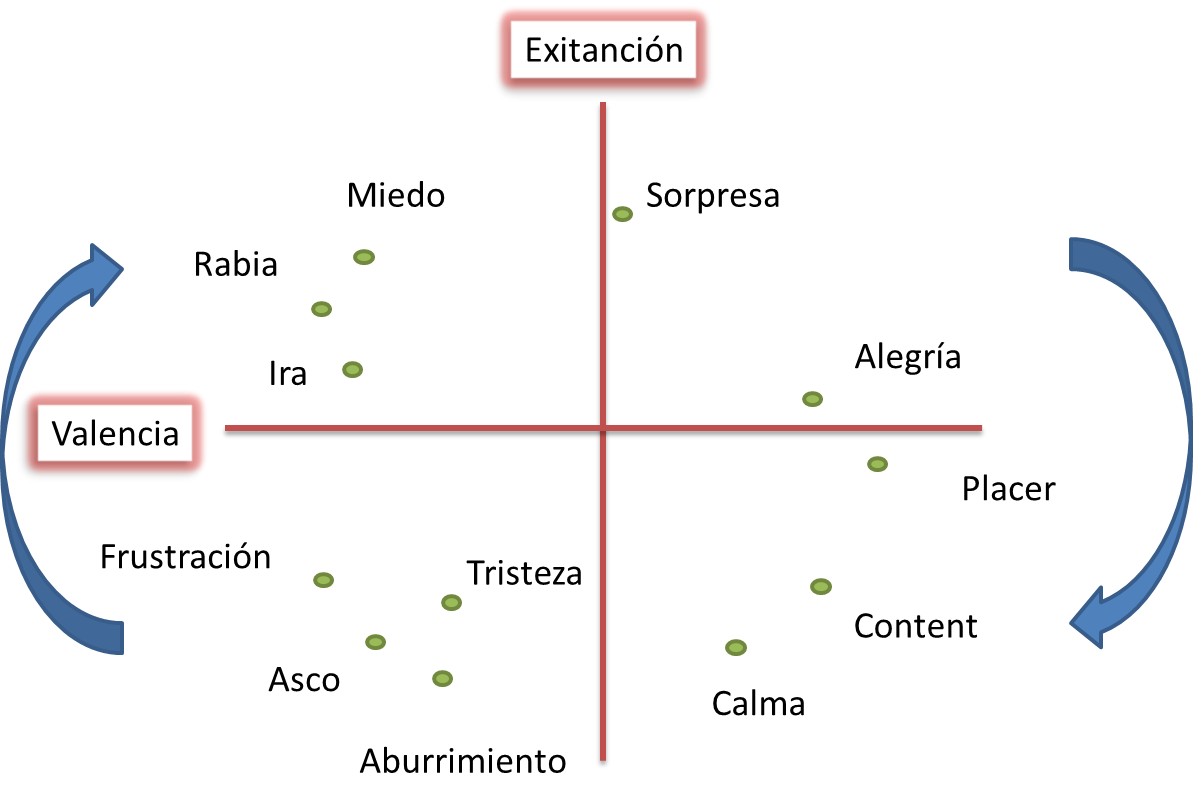
\includegraphics[width=.6\textwidth]{images/Two_Dimensions_of_Emotion.png}
	\caption[Representación de las emociones en 2 dimensiones]{Representación de las emociones en 2 dimensiones}
%(tomada de \cite{WikiEmotion})
	\label{F-dimensions-emotion}
\end{figure}

Este tipo de aplicaciones se han utilizado en la industria en empresas como los call centers en los cuales se utiliza para la detección automática de emociones, pero lo más importante de esto es que esta herramienta puede proporcionar a los operadores humanos información muy valiosa acerca de las emociones que su voz contiene. Dicho de otra forma, el sistema sirve de ``espejo emocional'' \cite{Pickard1997}. Recientemente, los métodos para reconocimiento de emociones en el habla han sido explorados en el contexto de aprendizaje aumentado por computador. La motivación detrás de esas aproximaciones es la expectativa que el proceso de aprendizaje puede mejorar si un sistema tutor adapta sus estrategias pedagógicas al estado emocional de sus estudiantes \cite{Ai2006}.\\

En adición, la detección de emociones tiene altos potenciales en juegos \cite{Jones2008} y sirve de realimentación en interacción humano-robot \cite{Jones2008a}. Generalmente, un sistema de reconocimiento de emoción a partir del habla, consta de tres componentes principales: procesamiento de la señal, cálculo de rasgos y clasificación. 
El procesamiento de la señal implica la digitalización y potencialmente procesamiento acústico como filtrado, así como la segmentación de la señal de entrada en unidades con significado. El cálculo de los rasgos se trata de la identificación de los rasgos relevantes de la señal acústica respecto de las emociones. La clasificación, finalmente, mapea los vectores de rasgos en clases de emociones a través de aprendizaje con ejemplos. \\

Se da por sentado que la primera fase mencionada anteriormente, está bien manejada y documentada \cite{Devillers2005}, \cite{Batliner2003}, \cite{Fernandez2005}, \cite{Nicholas2006}. El segundo paso mencionado como la extracción de rasgos de la señal, se ocupa de distinguir las propiedades de la señal acústica digitalizada y preprocesada que son característicos de las emociones y de representarlas en un vector de rasgos n-dimensional. Sin embargo, no existe consenso alguno sobre que rasgos son los más importantes y cuáles son los más dependientes de los datos. No obstante, un número muy grande de rasgos o características de las señal no siempre es beneficioso puesto que muchos clasificadores están influenciados negativamente por datos redundantes, correlacionados, o irrelevantes. En la literatura se han propuesto varios algoritmos, como análisis de componentes principales (PCA\nomenclature{PCA}{Análisis de componentes principales, por sus siglas en inglés}), coeficientes Formants and Mel Frequency Cepstral (MFCC\nomenclature{MFCC}{Mel-frequency cepstral coefficients}), medidas espectrales y representaciones parametricas diferentes a MFCC como las wavelets, operadores de energía de Teager (TEO\nomenclature{TEO}{Operadores de energía de Teager, por sus siglas en inglés}) y coeficientes cepstral de predicción lineal (LPCC\nomenclature{LPCC}{Coeficientes cepstral de predicción lineal, por sus siglas en inglés}). También se han usado clasificadores estadísticos como support vector machines (SVM\nomenclature{SVM}{Support vector machines}) o clasificadores dinámicos como modelos de markov ocultos (HMM\nomenclature{HMM}{Modelos de markov ocultos, por sus siglas en inglés}) \cite{Vogt2008}.\\

En la etapa de clasificación, la literatura propone que cada entrada sea un vector de rasgos, lo que convierte el problema de reconocimiento de emociones en un problema de minería de datos general. Las técnicas usadas a este respecto son básicamente clasificadores estadísticos, SVM, redes neuronales y árboles de decisión para rasgos generales y modelos de Markov para rasgos de corto plazo como una técnica de modelado dinámico ampliamente encontrada en la literatura \cite{Wagner2007}. Todos estos clasificadores necesitan datos para el aprendizaje de sus parámetros. \\

En la Facultad de Informática de la Universidad Politécnica de Madrid (UPM\nomenclature{UPM}{Universidad Politécnica de Madrid}) han desarrollado una aplicación que reconoce las emociones humanas a través del estudio automatizado de la voz. El programa es capaz de distinguir las emociones escondidas en una frase, determinando así el estado emocional de quién la pronuncia. La aplicación puede precisar, incluso si la emoción no está clara, el porcentaje de adecuación del hablante a cada emoción. ¿Cómo lo hace? Analizando las medidas sonoras de una conversación, que se obtienen con otro programa específico, y en base a las reglas descritas en la nueva aplicación, es capaz de distinguir las emociones escondidas en una frase, pudiendo determinar si la persona que la pronuncia está triste, asustada, alegre o nerviosa. Se basa en una herramienta conocida como RFuzzy, implementada sobre el lenguaje de programación Prolog, que es capaz de representar y trabajar con la así llamada lógica difusa. Prolog se usa principalmente en aplicaciones de Inteligencia Artificial y Sistemas Expertos \cite{Munoz-Hernandez2009}.\\

En la historia de las investigaciones de la inteligencia artificial, se han propuesto mucho modelos para describir la mente humana \cite{El-Nasr2000}, dada la naturaleza difusa de las emociones, la lógica difusa fue y sigue siendo una de las primeras herramientas explotadas para desarrollar modelos computacionales de la emoción. Yanaru \cite{Yanaru1997} uso la lógica difusa para definir la emoción mientras una persona leía un poema usando su estado emocional previo para inferir la nueva emoción. El-Nasr et al \cite{El-Nasr2000} propuso un modelo difuso para generar la emoción en una mascota virtual focalizándose en los componentes comportamentales y cognitivos de la emoción de manera que la mascota pudiera tomar sus propias decisiones y aprender las nuevas experiencias. Mandryk y Atkins \cite{Mandryk2007} proporciona un método para cuantificar los estados emocionales durante la interacción con juegos de video usando la componente fisiológica de la emoción, mapeando de medidas fisiológicas a valores de excitación-valencia y de excitación-valencia a cinco emociones.\\

Tradicionalmente los elementos para la ``detección de emociones'' a través de la voz se han construido por medio del tono y la intensidad (y en este sentido existen dificultades en cuanto a la determinación de un único estado emocional sólo con la voz). A partir de estos elementos se pueden identificar cambios en los registros ``asociados a cambios emocionales'', o niveles de activación emocional o de valencia emocional. La propuesta de paso de las señales a los planos podría mostrar cierta dificultad ya que, aunque pueden encontrarse elementos de activación, es un poco más difícil hallar elementos asociados a la valencia. En el caso del procesamiento de las señales para búsqueda de los rasgos basados en componentes espectrales de frecuencia, puede suceder que del procesamiento de señales se deriven unos rasgos que no necesariamente corresponda a valores de activación o de valencia. \\

Hay que tener presente que, dentro de las teorías de las emociones hay quienes sostiene la idea de entenderlas más en términos de las valoraciones de los estados, en ese sentido tendríamos emociones positivas y negativas (que podrían estar más asociadas, hipotéticamente, al tono de la voz), y niveles de activación o excitación (más asociados a la intensidad representada durante el estado). Es clave ver que del registro de voz es más fácil distinguir cambios de estados emocionales (cambios de una valencia a otra o cambio de una intensidad a otra) en ciertos momentos, y un poco más difícil determinar los estados emocionales propios (es decir, alegría, tristeza, etc.). Al final, el análisis del espectro de la señal deberá permitir derivar, dentro de los rasgos, valores asociados a la valencia y valores asociados a la intensidad, para general el plano en mención.\\

Es por ello que se hace necesaria la inclusión de un mecanismo que fusione los resultados de la minería de datos sobre la señal, y los extraídos del análisis espectral de la señal, con el fin de obtener un resultado sobre la conversación analizada. Este mecanismo de fusión será diseñado usando técnicas de inteligencia artificial que aprendan de un experto humano, a determinar si la situación presenta o no anomalías, usando la información disponible de las fases de análisis automático del audio.\\

Este proyecto de investigación busca plantear un desarrollo tecnológico que permita identificar, a partir de una base de datos real, la probabilidad de anomalías en las transacciones basados en el reconocimiento de emociones en el habla. Esta identificación se realizará mediante la aplicación de técnicas de procesamiento digital de la señal de audio y su conversión en texto para la posterior minería de datos usando un diccionario de palabras previamente proporcionado por el área de Compliance del Grupo Bancolombia. Paralelamente, las señales de audio serán procesadas en busca de los rasgos emocionales usando técnicas como las basadas en las componentes espectrales de frecuencia mediante wavelets-onditas, las basadas en teoría de la información, como entropía, complejidad, etc; que serán mapeados al plano excitación-valencia y finalmente ambas salidas serán fusionadas en un sistema de inferencia realizado con técnicas de Inteligencia artificial, que replicará el conocimiento de los expertos auditores y analistas de Compliance y proporcionará una salida que indique si tal o cuál conversación requiere un nivel superior de análisis, lo que implica una probabilidad más alta de ocurrencia de la anomalía.\\

Finalmente, el rol del trabajo de grado de ingeniería física busca materializar los desarrollos teórico-prácticos que los demás integrantes del equipo investigador realiza y continuará realizando. Este trabajo responde eficazmente a los requerimientos de usabilidad, portabilidad, adaptabilidad, tiempo real, seguridad, amigable con el usuario, y representa la herramienta de trabajo de campo que es el valor agregado de la investigación puesto que, en los objetivos iniciales de la investigación principal, solo se contempló el desarrollo tecnológico alrededor de una aplicación de software. Es así como la ingeniería física permitió superar las expectativas propias del proyecto de investigación del que hace parte este trabajo de grado.\\

En este documento se expone el resultado del trabajo. en la \seccion{S-problema} se presenta el problema que se trató, los objetivos del proyecto de grado, su justificación y la metodología propuesta en el anteproyecto. En la \seccion{S-diseño} se muestra el proceso de diseño conceptual desarrollado en el trabajo y el marco teórico asociado al fenómeno físico y al problema planteado. La \seccion{S-hardware} expone las características del hardware con el que se trabajó, del software empleado y desarrollado para el proyecto se ocupa la \seccion{S-software}. La \seccion{S-resultado} presenta el resultado de este proyecto y su validación. Finalmente, la \seccion{S-conclusiones} enumera las conclusiones del proyecto y el trabajo futuro propuesto.


%----------------- Planteamiento del problema ------------------------%
\cleardoublepage
\section{Problema}
\label{S-problema}
\subsection{Planteamiento del problema}
%------------------------ Estado del arte ----------------------------%
%\section{Estado del arte}

%Actualmente en la Universidad EAFIT se lleva a cabo el proyecto de investigación ``\emph{Reconocimiento de emociones}''. En términos generales, busca elaborar una herramienta tecnológica, desarrollada a la medida de la investigación, que identifique los cambios del estado emocional de un interlocutor en una grabación, por medio de la obtención de algunas características de la señal de audio. Los rasgos más importantes para distinguir entre diferentes emociones de acuerdo a la percepción humana son los parámetros vocales de prosodia (tono, intensidad y velocidad de habla) y calidad de la voz, más particularmente el tono y la intensidad, como se muestra en la revisión bibliográfica elaborada por Murray y Arnott \cite{Murray1993}. \\
%
%En la investigación. en la que este proyecto se enmarca, se plantean modelos que buscan representar los rasgos extraídos de la señal de audio en un espacio donde se encuentran las emociones más importante de los seres humanos. Los cuales, permiten una descripción continua de las mismas, lo que es muy válido al considerar emociones espontáneas. Las dimensiones de este espacio son principalmente valencia o bienestar (de positiva a negativa) y excitación o activación (de alta a baja), algunas veces se plantea una tercera dimensión llamada postura (de abierta a cerrada) \cite{Russell1979},\cite{Russell1980},\cite{Russell1989},\cite{Russell1999}. En la \figura{F-dimensions-emotion} se muestra un ejemplo de la representación en 2 dimensiones.\\
%
%\begin{figure}[h!]
%	\centering
%	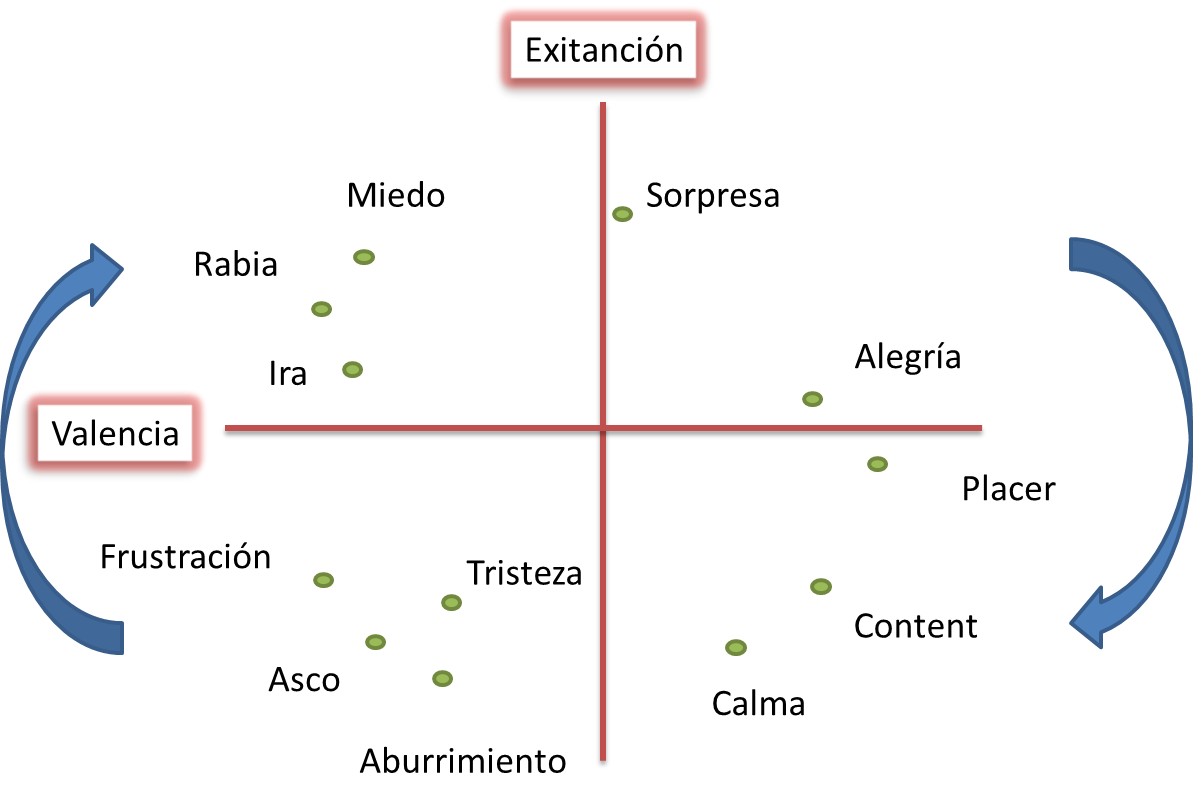
\includegraphics[width=.6\textwidth]{images/Two_Dimensions_of_Emotion.png}
%	\caption[Representación de las emociones en 2 dimensiones]{Representación de las emociones en 2 dimensiones}
%%(tomada de \cite{WikiEmotion})
%	\label{F-dimensions-emotion}
%\end{figure}
%
%Generalmente, los sistemas de reconocimiento de emociones a partir del habla encontrados en la bibliografía, consisten de tres componentes principales: pre-procesamiento de la señal, cálculo de rasgos y clasificación. El pre-procesamiento contiene la adquisición, digitalización y de ser necesario la adecuación la señal, un procesamiento acústico como el filtrado y la segmentación de la señal de entrada en paquetes a través de un \textit{buffer}. En este punto es necesario tener en cuenta la documentación existente \cite{Devillers2005}, \cite{Batliner2003}, \cite{Fernandez2005}, \cite{Nicholas2006}. La siguiente etapa, el procesamiento, trata de la identificación de los rasgos relevantes de la señal acústica respecto de las emociones, ya sea en el espectro del tiempo o de la frecuencia. Por último se clasifican los rasgos encontrados en grupos de emociones. A pesar de que el objetivo de la investigación es elaborar una herramienta tecnológica, es de gran ayuda la construcción de un dispositivo que implemente el desarrollo y que permita mayor versatilidad y facilidad en el transporte, para la realización de pruebas y demostraciones. \\
%
%En la patente WO2000062279 titulada \textit{apparatus and methods for detecting emotions in the human voice} \cite{Liberman2000} se describe el algoritmo y los componentes principales de un dispositivo que permite reconocer el estado emocional de un sujeto, los cuales son ya bien conocidos en el tratamiento de señales, una etapa de adquisición, una de digitalización, una de procesamiento, una de clasificación y una de reporte de resultados. \\

%cual es el valor agregado? aqui debe quedar plasmado el corazon del trabajo suyo.

Dadas las condiciones expuestas anteriormente, el problema central a resolver en este trabajo es el diseño y desarrollo del prototipo de un dispositivo capaz de analizar señales de audio por medio de la transformada wavelet, con miras al reconocimiento de emociones. Para lo cual es necesario diseñar y construir, mediante los conocimientos aprendidos en el pregrado de ingeniería física, un hardware capaz de adquirir, digitalizar, pre-procesar, procesar por medio del análisis wavelet y reportar los resultados encontrados. Este dispositivo además debe ser extendible, de modo que pueda realizar fases de clasificación y reporte de las emociones a partir de una señal de audio, estas se proponen como trabajo futuro (\seccion{S-trabajofuturo}).

%----------------- Objetivos de la propuesta -------------------------%
\subsection{Objetivos}
\subsubsection{General}
Diseñar y construir un prototipo para análisis de señales de audio por medio de la transformada wavelet orientado al reconocimiento de emociones, en el contexto de la investigación ``\emph{Reconocimiento de Emociones}''
\subsubsection{Específicos}
\begin{enumerate}
	\item Elaborar el diseño conceptual del dispositivo, partiendo de la identificación de los requerimientos técnicos y del usuario.
	\item Diseñar las etapas de adquisición, pre-procesamiento y procesamiento de la señal de audio.
%	\item Diseñar y desarrollar el algoritmo de análisis de la señal.
	\item Construir la planta física y verificar la correcta comunicación entre los periféricos utilizados.
	\item Digitalizar la señal de audio por medio del convertidor analógico digital escogido en el diseño conceptual, teniendo en cuenta el análisis espectral de la señal fenomenológica aplicando conceptos básicos de muestreo y retención de datos.
	\item Desarrollar los algoritmos de pre-procesamiento y procesamiento de la señal.
%	\item Implementar filtros para la señal adquirida.
	\item Implementar los algoritmos desarrollados.
	\item Realizar pruebas del dispositivo piloto final para evaluar su desempeño, por medio de la comparación con herramientas de programación ya validadas o datos reportados en la literatura.
\end{enumerate}

%---------------- Justificación de la propuesta ----------------------%
\subsection{Justificación}
Es evidente que las emociones percibidas son un aspecto muy importante en el desarrollo humano y cumplen un papel significativo en la toma de decisiones. Debido a ello existen herramientas tecnológicas que se han utilizado en empresas como los \textit{call centers}, donde se aplican a la identificación de las emociones que refleja la voz de los operadores con el fin de brindarles información sobre lo que el cliente percibe y así proveer un mejor servicio. Además de ello, su implementación en juegos de video e interacciones humano-dispositivo (celulares, robots o cualquiera con interacción basada en voz o gesticulación), puede llevar al mejoramiento de la experiencia, incluso podría ayudar a superar el \textit{uncanny valley} de la robótica y la animación por computadora, esta hipótesis afirma que cuando una una figura antropomórfica actúa muy similar a los humanos reales, causan una respuesta de rechazo entre estos últimos \cite{Woods2004}. \\

Por parte del proyecto de investigación principal, se ve la necesidad de un dispositivo funcional que implemente los desarrollos realizados hasta el momento, y que permita agregarle fácilmente hallazgos posteriores; de manera que el prototipo sirva para realizar pruebas piloto para proyecto. Por otra parte, el desarrollo de este proyecto abarca conocimientos de diseño conceptual, programación, electrónica,  instrumentación básica y tratamiento de señales donde se puede observar el fundamento ingenieril de la línea de proyectos carrera. Además de la formulación, dimensionamiento, evaluación y desarrollo de proyectos, elementos también adquiridos en la misma línea. Adicionalmente se requieren conocimientos del fenómeno físico a tratar y de matemáticas aplicadas. De esta manera la solución al problema planteado logra conectar múltiples líneas dentro de la Ingeniería Física.

%------------------------- Metodología -------------------------------%
\subsection{Metodología}
%Exponer la idea original y los cambios que se fueron dando. Curva S?
Para la solución de este problema se plantearon 3 etapas donde se desarrollaron los objetivos. En la primera etapa se realizó una búsqueda bibliográfica relacionada con el proyecto y luego se identificaron los requerimientos de usuario, llevó a cabo el diseño conceptual del dispositivo y la seleccionar los componentes técnicos necesarios. Esta etapa buscaba definir la instrumentación necesaria para la construcción del prototipo, el lenguaje de programación y el esquema del software a desarrollar. \\

La segunda etapa fue la construcción del dispositivo según los resultados arrojados por el diseño conceptual. Primero se consideró cada elemento del hardware por separado y luego de garantizar su funcionamiento aislado, se procedió a acoplar las partes, para luego verificar la comunicación y operación del hardware como un todo. La tercera etapa abarcaba el software, comenzando con el diseño del mismo, para continuar con la programación y puesta a punto de los algoritmos. Al culminar está etapa se esperaba contar con código versátil, listo para su implementación en el hardware del dispositivo. Posteriormente se planeó realizar la evaluación del prototipo por medio de la comparación con herramientas de programación ya validadas o datos reportados en la literatura y finalmente elaborar la documentación pertinente.\\

En la metodología también se planeó emplear herramientas de desarrollo libre con el fin de proveer un dispositivo de bajo costo y evitar percances en el transcurso del proyecto.\\

%------------------------- Cronograma --------------------------------%
\textbf{Cronograma propuesto y curva S}
El tiempo de ejecución del proyecto comienzó el 22 de julio de 2013 (segunda semana del periodo lectivo), el cronograma planeado, semana por semana, al inicio de la ejecución del proyecto se muestra en la tabla \tabla{cronograma} y en la \figura{F-s-curve} se observa la curva S del proyecto, la cual es una comparación entre el desarrollo planeado y el desarrollo ejecutado, los retrasos sufridos se debieron principalmente a la complejidad de los temas y a agentes externos al proyecto.
\begin{table}[H]
\begin{center}
\resizebox{\textwidth}{!}{
\begin{tabular}{|c|c|c|c|c|c|c|c|c|c|c|c|c|c|c|c|c|}
\hline
\multirow{3}{*}{\textbf{Objetivo}} & \multirow{3}{*}{\textbf{Actividad}} & \multicolumn{15}{|c|}{\textbf{Semana}} \\ \cline{3-17}

& & & \multicolumn{5}{|c|}{Agosto} & \multicolumn{4}{|c|}{Septiembre} & \multicolumn{5}{|c|}{Octubre} \\ \cline{3-17}

& & 2 & 3 & 4 & 5 & 6 & 7 & 8 & 9 & 10 & 11 & 12 & 13 & 14 & 15 & 16 \\ \hline

\multirow{4}{*}{Diseño conceptual} & Revisión de bibliografía & \cellcolor[gray]{0.6} &\cellcolor[gray]{0.6} &\cellcolor[gray]{0.6} & & & & & & & & & & & & \\ \cline{2-17}
& Identificación de los requerimientos de usuario & &\cellcolor[gray]{0.6} & & & & & & & & & & & & & \\ \cline{2-17}
& Consideración de opciones (Matriz morfológica) & &\cellcolor[gray]{0.6} &\cellcolor[gray]{0.6} & & & & & & & & & & & & \\ \cline{2-17}
& Selección y compra de elementos & & &\cellcolor[gray]{0.6}&\cellcolor[gray]{0.6} &\cellcolor[gray]{0.6} &\cellcolor[gray]{0.6} &\cellcolor[gray]{0.6} & & & & & & & & \\ \hline

\multirow{4}{*}{Algoritmos} & Diseño de los algoritmos a utilizar & & &\cellcolor[gray]{0.6} &\cellcolor[gray]{0.6} &\cellcolor[gray]{0.6} & & & & & & & & & & \\ \cline{2-17}
& Programación de los módulos & & & &\cellcolor[gray]{0.6} &\cellcolor[gray]{0.6} & & & & & & & & & & \\ \cline{2-17}
& Pruebas de los módulos & & & & &\cellcolor[gray]{0.6} &\cellcolor[gray]{0.6} &\cellcolor[gray]{0.6} &\cellcolor[gray]{0.6} & & & & & & & \\ \cline{2-17}
& Verificación y retroalimentación de módulos & & & & & &\cellcolor[gray]{0.6} &\cellcolor[gray]{0.6} &\cellcolor[gray]{0.6} & & & & & & & \\ \hline

\multirow{5}{*}{Construcción e implementación} & Montaje de hardware por componentes & & & & & & &\cellcolor[gray]{0.6} &\cellcolor[gray]{0.6} &\cellcolor[gray]{0.6} &\cellcolor[gray]{0.6} & & & & & \\ \cline{2-17}
& Unificación del hardware & & & & & & & & \cellcolor[gray]{0.6}& \cellcolor[gray]{0.6}& \cellcolor[gray]{0.6}& \cellcolor[gray]{0.6}& \cellcolor[gray]{0.6}& & & \\ \cline{2-17}
& Adquisición y digitalización de la señal & & & & & & & & &\cellcolor[gray]{0.6} &\cellcolor[gray]{0.6} &\cellcolor[gray]{0.6} & & & & \\ \cline{2-17}
& Implementación de los algoritmos & & & & & & & & & &\cellcolor[gray]{0.6} &\cellcolor[gray]{0.6} &\cellcolor[gray]{0.6} &\cellcolor[gray]{0.6} & & \\ \cline{2-17}
& Pruebas de desempeño (algoritmo – hardware) & & & & & & & & & & &\cellcolor[gray]{0.6} &\cellcolor[gray]{0.6} &\cellcolor[gray]{0.6} &\cellcolor[gray]{0.6} & \\ \hline

\multirow{1}{*}{Pruebas de desempeño} & Pruebas del dispositivo y corrección de errores & & & & & &\cellcolor[gray]{0.6} &\cellcolor[gray]{0.6} &\cellcolor[gray]{0.6} &\cellcolor[gray]{0.6} &\cellcolor[gray]{0.6} &\cellcolor[gray]{0.6} &\cellcolor[gray]{0.6} &\cellcolor[gray]{0.6} &\cellcolor[gray]{0.6} & \\ \hline

- & Documentación &\cellcolor[gray]{0.6} &\cellcolor[gray]{0.6} &\cellcolor[gray]{0.6} &\cellcolor[gray]{0.6} &\cellcolor[gray]{0.6} &\cellcolor[gray]{0.6} &\cellcolor[gray]{0.6} &\cellcolor[gray]{0.6} &\cellcolor[gray]{0.6} &\cellcolor[gray]{0.6} &\cellcolor[gray]{0.6} &\cellcolor[gray]{0.6} &\cellcolor[gray]{0.6} &\cellcolor[gray]{0.6} &\cellcolor[gray]{0.6} \\ \hline
\end{tabular} }
\end{center}
\caption{Cronograma de actividades}
\label{cronograma}
\end{table}
\begin{figure}[h!]
	\centering
	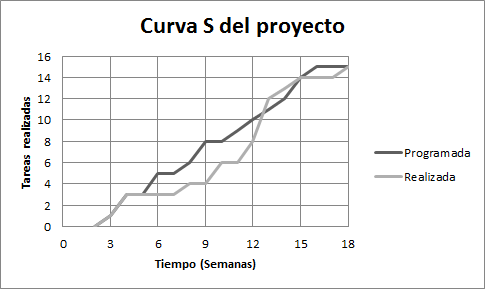
\includegraphics[width=.8\textwidth]{images/s-curve.png}
	\caption{Curva S del proyecto}
	\label{F-s-curve}
\end{figure}


%------------------ Conceptual design  (Capítulo) --------------------%
%----------------------- Revisión teórica ----------------------------%
\cleardoublepage
\section{Diseño conceptual y marco teórico}
\label{S-diseño}
%Revisión teórica
%- Conversión ADC
%- Transformada de fourier ??
%- Transformada wavelet (Efficient Implementations of Discrete Wavelet Transforms Using FPGAs)
%- Complejidad algoritmica ??
%- Algoritmo (Seudocódigo) ??
%- voz humana y emociones
%- Filtros


% Diseño conceptual
% - Estructura (~Planteamiento del problema)
% - Requerimientos
% - Valoración de requerimientos (1-5)
% - Matriz morfológica
% - Ruta

%Trabajos en FPGAs:
%Efficient Implementations of Discrete Wavelet Transforms Using FPGAs
%http://etd.lib.fsu.edu/theses/available/etd-11242003-185039/
%
%Wavelet Transform Based Image Compression on Fpga
%http://etd.lib.fsu.edu/theses/available/etd-04062004-225402/
%
%Design of Custom Instruction Set for FFT using FPGA-Based Nios Processors
%http://etd.lib.fsu.edu/theses/available/etd-06262004-162018/
%
%Implementation of Chirp z DFT on Virtex II FPGA
%http://etd.lib.fsu.edu/theses/available/etd-04202004-002332/
%
%FPGA Implementation Of Digital Filters Using MCM
%http://etd.lib.fsu.edu/theses/available/etd-05112010-163813/
%
%Adaptive Filter Architectures For FPGA Implementation
%http://etd.lib.fsu.edu/theses/available/etd-07062004-133258/
%
%Sparse FIR Filters And The Impact On FPGA Area Usage
%etd.lib.fsu.edu/theses/available/etd-12112008-135228/

Esta sección del documento muestra el diseño conceptual elaborado para el desarrollo del proyecto y los conceptos teóricos alrededor de las fases. La etapa de diseño conceptual se basó en las propuestas por Ulrich \cite{Ulrich2011} y por Pahl et al. \cite{Pahl2007}.  El dispositivo que se desea diseñar debe analizar el fenómeno físico de la propagación de una onda de sonido que bajo sus características porta información sobre el estado de animo de la persona que emite dicha onda, para realizarlo adecuadamente se deberá transitar por diferentes fases: adquisición y digitalización, almacenamiento, filtrado de la señal, generación de gráficas para dar información sobre la señal y finalmente, análisis wavelet; los resultados de esta operación serán gráficas que reporten la información de la señal en tiempo y frecuencia, y archivos de texto plano que contengan los resultados del análisis wavelet. Para el reconocimiento de emociones es necesario realizar una fase adicional de toma de decisiones sobre los análisis elaborados. La \figura{F-diagrama-fases} muestra el esquema de estas fases, en gris las comprendidas en este proyecto y en azul la propuesta como trabajo futuro (\seccion{S-trabajofuturo}), estas serán expuestas más detalladamente en las siguientes subsecciones.

\begin{figure}[h!]
	\centering
	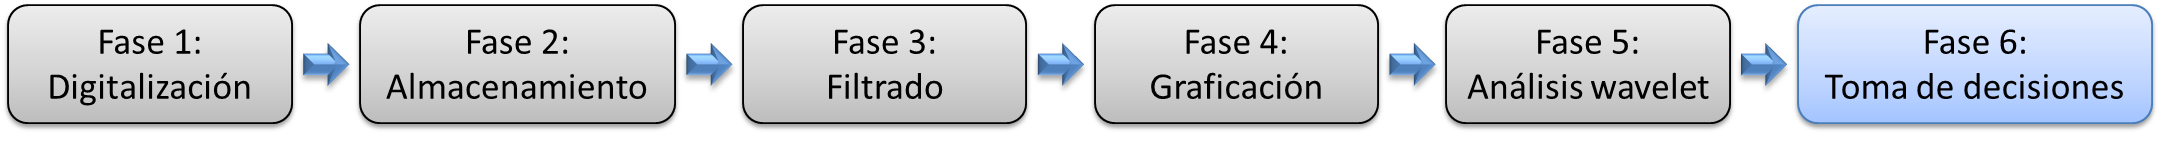
\includegraphics[width=1\textwidth]{images/diagrama-fases.png}
	\caption{Diagrama de fases necesarias para realizar la tarea}
	\label{F-diagrama-fases}
\end{figure}


\subsection{Fenómeno físico}
%(esta herramienta no se expondrá en el marco teórico del proyecto debido a que es bien conocida en la ciencia y la ingeniería)
El fenómeno físico desarrollado en este proyecto es la propagación de información a través de una onda sonora, donde la información son las emociones que expresa un interlocutor y las características de la señal de audio son los datos para trabajar.\\

La música requiere un ancho de banda de 20kHz, mientras el sonido de la voz humana en un discurso normal sólo requiere 3.2kHz; aunque la frecuencia se disminuye al 16\%, la señal aún contiene el 80\% de la información de la onda inicial de sonido. Por otra parte, los sistemas de telecomunicaciones operan típicamente con una Fs de 8kHz (FN de 4kHz) permitiendo una comunicación efectiva \cite{Smith1997}. Adicional a la bibliografía, en el proyecto se realizó un análisis de audio con el fin de verificar cuales eran las Fs necesarias para cubrir adecuadamente el fenómeno físico. Este análisis se basó en aplicar diferentes Fs, filtros, \textit{resampling} (cambio de Fs) y análisis de Fourier. En la \figura{F-rate-quality} se presenta una comparación entre las Fs, su utilización y la calidad del audio adquirido.
\begin{figure}[H]
	\centering
	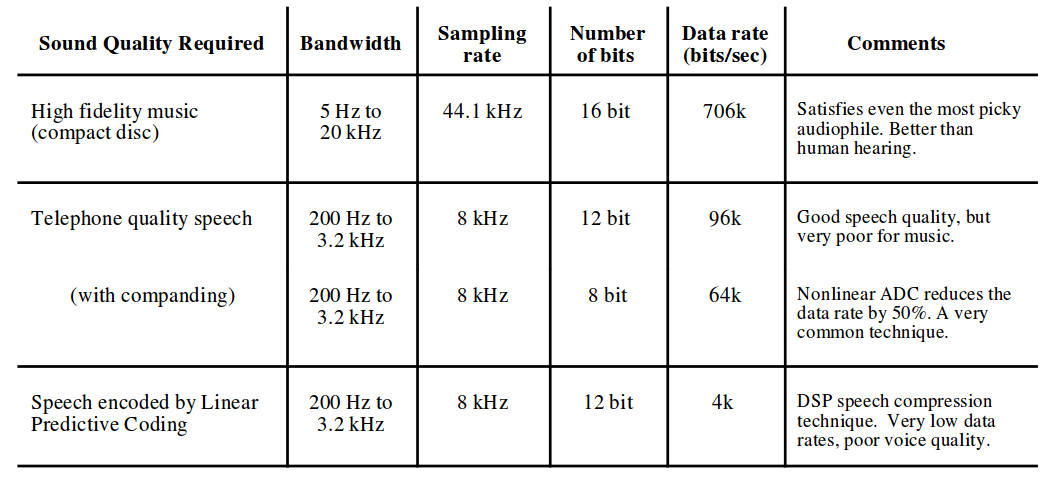
\includegraphics[width=1\textwidth]{images/rate-quality.png}
	\caption[Tasa de muestreo (Fs) y calidad del sonido]{Tasa de muestreo (Fs) y calidad del sonido (tomada de \cite{Smith1997})}
	\label{F-rate-quality}
\end{figure}

%Whereas music requires a bandwidth of 20 kHz, natural sounding speech only
%requires about 3.2 kHz. Even though the frequency range has been reduced to
%only 16% (3.2 kHz out of 20 kHz), the signal still contains 80% of the original
%sound information (8 out of 10 octaves).Telecommunication systems typically
%operate with a sampling rate of about 8 kHz, allowing natural sounding speech,
%but greatly reduced music quality.


%Analisis de Fourier (lo que me llevo a A/D)
%  NO ENTIENDO
%  FFT
%  analisis de audio


\subsection{Propuesta de diseño}
\label{S-prop-dise}
Además de cumplir su tarea sobre el fenómeno físico, el prototipo deberá seguir unos requerimientos de usuario y unos técnicos. Se concibe al usuario de este dispositivo como personas interesadas en utilizarlo para el reconocimiento de emociones a partir de un análisis wavelet o a personas que deseen realizar dicho análisis para otros fines; debido a que este trabajo surgió en el marco del proyecto ``\emph{Reconocimiento de emociones}'', son las personas de este, quienes especificaron los requerimientos de usuario, estos se muestran en \tabla{T-req-usuario}. Los requerimientos técnicos fueron basados en el funcionamiento final, el tiempo de ejecución del proyecto y el fenómeno físico; son mostrados en la \tabla{T-req-tecnicos}. En las tablas cada requerimientos se presenta junto a su nivel de importancia, siendo 1 el más importante y va hasta el número de requerimientos, 11 de usuario y 7 técnicos. Hay requerimentos técnicos que sólo aplican para ciertos componentes, estos son: múltiples frecuencias de muestreo para la fase de digitalización, capacidad de procesamiento y hardware adicional para las demás fases, y finalmente, disposición de librerías wavelet para fase de análisis wavelet.
%\begin{itemize}[nolistsep]
%	\item Funcional
%	\item Autónomo
%	\item Eficiente con las tareas
%	\item Eficaz con las tareas
%	\item Software abierto
%	\item Reprogramable
%	\item Amigable con el usuario
%	\item Seguro
%	\item Fácil transporte
%	\item Fácil instalación
%	\item Bajo costo
%\end{itemize}
\begin{table}[H]
	\begin{center}
	% \resizebox{\textwh}
		\begin{tabular}{|c|c|}
			\hline
			{\textbf Requerimiento} & {\textbf Nivel} \\ \hline
			Funcional & 1 \\ \hline
			Autónomo & 7 \\ \hline
			Eficiente con las tareas & 8 \\ \hline
			Eficaz con las tareas & 9 \\ \hline
			Software abierto & 2 \\ \hline
			Reprogramable & 3 \\ \hline
			Amigable con el usuario & 6 \\ \hline
			Seguro & 5 \\ \hline
			Fácil transporte & 10 \\ \hline
			Fácil instalación & 11 \\ \hline
			Bajo costo & 4 \\ \hline
		\end{tabular}
		\caption{Requerimientos de usuario del prototipo}
		\label{T-req-usuario}
	\end{center}
\end{table}

%\begin{itemize}[nolistsep]
%	\item Tiempo de desarrollo corto
%	\item Fácil apropiación del conocimiento necesario
%	\item Elementos asequibles
%\end{itemize}
\begin{table}[H]
	\begin{center}
	% \resizebox{\textwh}
		\begin{tabular}{|c|c|}
			\hline
			{\textbf Requerimiento} & {\textbf Nivel} \\ \hline
			Tiempo de desarrollo corto & 4 \\ \hline
			Aprendizaje rápido & 3 \\ \hline
			Disponibilidad en el mercado & 1 \\ \hline
			Librerías wavelet & 2 \\ \hline
			Capacidad de procesamiento & 5 \\ \hline
			Hardware adicional & 6 \\ \hline
			Múltiples frecuencias de muestreo & 7 \\ \hline
		\end{tabular}
		\caption{Requerimientos técnicos del prototipo}
		\label{T-req-tecnicos}
	\end{center}
\end{table}

Según estos requerimientos se escogieron unos elementos iniciales, con los cuales se realizó la matriz morfológica mostrada en la \tabla{T-matriz}, en ella se muestran los componentes que cumplirían cada fase, periféricos de entrada, realiza la adquisición, y periférico de salida, muestra los resultados; algunos elementos de las fases de procesamiento (2-6) no requieren una digitalización independiente, esto fue tenido en cuenta por medio del requerimiento de \emph{Hardware adicional}. Posteriormente se realizó una valoración de los elementos, su resultado se expone en la \tabla{T-valor-mic} para el periférico de entrada, \tabla{T-valor-adc} para la fase de digitalización, \tabla{T-valor-proc} para las demás fases y \tabla{T-valor-display} para el periférico de salida; la columna de requerimientos está ordenada según el nivel de importancia y en ella sólo aparecen los requerimientos pertinentes para cada grupo de componentes, esto se debe a que hay requerimientos que no dependen de los componentes sino de otros elementos como la programación. Al ser este un proyecto desarrollado en un semestre lectivo (4 meses desde la formulación del proyecto hasta la entrega final), los requerimientos técnicos fueron tenidos en cuenta fuertemente debido al factor tiempo.
\begin{table}[H]
	\begin{center}
		\resizebox{\textwidth}{!}{
			\begin{tabular}{|c|c|ccccc|c|}
				\hline
				\multirow{2}{*}{\textbf{Periférico de entrada}} & \multicolumn{6}{c|}{\textbf{Fases}} & \multirow{2}{*}{\textbf{Periférico de salida}} \\ \cline{2-7}
%
%				& \textbf{Digitalización} & \multicolumn{1}{c|}{\textbf{Almacenamiento}} & \multicolumn{1}{c|}{\textbf{Filtrado de la señal}} & \multicolumn{1}{c|}{\textbf{Generación de gráficas}} & \multicolumn{1}{c|}{\textbf{Análisis wavelet}} & \multicolumn{1}{c|}{\textbf{Toma de decisiones}} & \\ \hline
				& \textbf{1} & \multicolumn{1}{c|}{\textbf{2}} & \multicolumn{1}{c|}{\textbf{3}} & \multicolumn{1}{c|}{\textbf{4}} & \multicolumn{1}{c|}{\textbf{5}} & \multicolumn{1}{c|}{\textbf{6}} & \\ \hline
%
%				& FPGA & \multicolumn{5}{c|}{\multirow{2}{*}{FPGA}} & \\ \cline{2-2}
%
				& \multirow{2}{*}{ADC Click} & \multicolumn{5}{c|}{FPGA} & \\ \cline{3-7}
%
%				& DSP & \multicolumn{5}{c|}{\multirow{2}{*}{DSP}} & \\ \cline{2-2}
%
				&& \multicolumn{5}{c|}{DSP} & \\ \cline{2-7}
%
				\multirow{3}{*}[13mm]{Ensamblar el micrófono} & \multirow{2}{*}{Conversor Stereo A/D} & \multicolumn{5}{c|}{DSPic} & \multirow{3}{*}[13mm]{Display alfanumérico} \\ \cline{1-1} \cline{3-8}
%
				&& \multicolumn{5}{c|}{Raspberry Pi (Rpi\nomenclature{Rpi}{Raspberry Pi\textregistered})} & \\ \cline{2-7}
%
				&\multirow{2}{*}{Tarjeta de sonido USB}& \multicolumn{5}{c|}{Arduino} & \\ \cline{3-7}
%
				\multirow{3}{*}[13mm]{Micrófono comercial} && \multicolumn{5}{c|}{Microcontrolador} & \multirow{3}{*}[13mm]{Display Gráfico}\\ \hline
			\end{tabular}
		}
	\caption{Matriz morfológica}
	\label{T-matriz}
	\end{center}
\end{table}

\begin{table}[H]
	\begin{center}
		\resizebox{\textwidth}{!}{
			\begin{tabular}{|c|c|c|c|}
				\hline
				\textbf{Tipo de requerimiento} & \textbf{Requerimiento} & \textbf{Armar el micrófono} & \textbf{Micrófono comercial} \\ \hline
				\multirow{1}{*}{Usuario} & Bajo costo & 5 & 4 \\ \hline
				\multirow{3}{*}{Técnico} & Disponibilidad en el mercado & 4 & 5 \\ \cline{2-4}
				& Aprendizaje rápido & 4 & 5 \\ \cline{2-4}
				& Tiempo de desarrollo corto & 4 & 5 \\ \hline
				\multicolumn{2}{|c|}{\textbf{Total}} & 17 & 19 \\ \hline
			\end{tabular}
		}
	\caption{Valoración del periféricos de entrada}
	\label{T-valor-mic}
	\end{center}
\end{table}

\begin{table}[H]
	\begin{center}
		\resizebox{\textwidth}{!}{
			\begin{tabular}{|c|c|c|c|c|}
				\hline
				\textbf{Tipo de requerimiento} & \textbf{Requerimiento} & \textbf{ADC Click} & \textbf{Conversor Stereo A/D} & \textbf{Tarjeta de sonido USB} \\ \hline
				\multirow{1}{*}{Usuario} & Bajo costo & 4 & 5 & 5 \\ \hline
				\multirow{4}{*}{Técnico} & Disponibilidad en el mercado & 5 & 5 & 5 \\ \cline{2-5}
				& Aprendizaje rápido & 5 & 4 & 5 \\ \cline{2-5}
				& Tiempo de desarrollo corto & 4 & 4 & 4 \\ \cline{2-5}
				& Multiples frecuencias de muestreo & 5 & 3 & 3 \\ \hline
				\multicolumn{2}{|c|}{\textbf{Total}} & 23 & 21 & 22 \\ \hline
			\end{tabular}
		}
	\caption{Valoración de la fase de digitalización}
	\label{T-valor-adc}
	\end{center}
\end{table}

\begin{table}[H]
	\begin{center}
		\resizebox{\textwidth}{!}{
			\begin{tabular}{|c|c|c|c|c|c|c|c|}
				\hline
				\textbf{Tipo de requerimiento} & \textbf{Requerimiento} & \textbf{FPGA} & \textbf{DSP} & \textbf{DSPic} & \textbf{Raspberry Pi} & \textbf{Arduino} & \textbf{Microcontrolador} \\ \hline
				\multirow{4}{*}{Usuario} & Software abierto & 3 & 3 & 5 & 5 & 5 & 5 \\ \cline{2-8}
				& Reprogramable & 5 & 5 & 5 & 5 & 5 & 5 \\ \cline{2-8}
				& Bajo costo & 2 & 3 & 5 & 4 & 5 & 5 \\ \cline{2-8}
				& Amigable con el usuario & 2 & 2 & 3 & 4 & 4 & 3 \\ \hline
				\multirow{6}{*}{Técnico} & Disponibilidad en el mercado & 3 & 3 & 5 & 5 & 5 & 5 \\ \cline{2-8}
				& Librerías wavelet & 2 & 3 & 5 & 5 & 0 & 5 \\ \cline{2-8}
				& Aprendizaje rápido & 0 & 1 & 2 & 3 & 3 & 3 \\ \cline{2-8}
				& Tiempo de desarrollo corto & 0 & 1 & 2 & 5 & 4 & 2 \\ \cline{2-8}
				& Capacidad de procesamiento & 5 & 5 & 5 & 3 & 1 & 1 \\ \cline{2-8}
				& Hardware adicional & 4 & 4 & 2 & 2 & 2 & 2 \\ \hline
				\multicolumn{2}{|c|}{\textbf{Total}} & 26 & 30 & 39 & 41 & 34 & 36 \\ \hline
			\end{tabular}
		}
	\caption{Valoración de las fases 2-6}
	\label{T-valor-proc}
	\end{center}
\end{table}

\begin{table}[H]
	\begin{center}
		\resizebox{\textwidth}{!}{
			\begin{tabular}{|c|c|c|c|}
				\hline
				\textbf{Tipo de requerimiento} & \textbf{Requerimiento} & \textbf{Display alfanumérico} & \textbf{Display Gráfico} \\ \hline
				\multirow{2}{*}{Usuario} & Bajo costo & 5 & 2 \\ \hline
				& Amigable con el usuario & 0 & 5 \\ \hline
				\multirow{3}{*}{Técnico} & Disponibilidad en el mercado & 5 & 5 \\ \cline{2-4}
				& Aprendizaje rápido & 5 & 4 \\ \cline{2-4}
				& Tiempo de desarrollo corto & 4 & 4 \\ \hline
				\multicolumn{2}{|c|}{\textbf{Total}} & 19 & 20 \\ \hline
			\end{tabular}
		}
	\caption{Valoración del periférico de salida}
	\label{T-valor-display}
	\end{center}
\end{table}

Finalmente, con las valoraciones de los componentes se propuso la ruta mostrada en gris en la \tabla{T-matriz-ruta-propuesta}.
%\cellcolor[gray]{0.7}

% \makeatletter
% \setlength{\@fptop}{0pt}
% \makeatother

\begin{table}[ht!]
	\begin{center}
		\resizebox{\textwidth}{!}{
			\begin{tabular}{|c|c|ccccc|c|}
				\hline
				\multirow{2}{*}{\textbf{Periférico de entrada}} & \multicolumn{6}{c|}{\textbf{Fases}} & \multirow{2}{*}{\textbf{Periférico de salida}} \\ \cline{2-7}
%
%				& \textbf{Digitalización} & \multicolumn{1}{c|}{\textbf{Almacenamiento}} & \multicolumn{1}{c|}{\textbf{Filtrado de la señal}} & \multicolumn{1}{c|}{\textbf{Generación de gráficas}} & \multicolumn{1}{c|}{\textbf{Análisis wavelet}} & \multicolumn{1}{c|}{\textbf{Toma de decisiones}} & \\ \hline
				& \textbf{1} & \multicolumn{1}{c|}{\textbf{2}} & \multicolumn{1}{c|}{\textbf{3}} & \multicolumn{1}{c|}{\textbf{4}} & \multicolumn{1}{c|}{\textbf{5}} & \multicolumn{1}{c|}{\textbf{6}} & \\ \hline
%
				& \cellcolor[gray]{0.7} & \multicolumn{5}{c|}{FPGA} & \\ \cline{3-7}
%
				& \cellcolor[gray]{0.7}\multirow{2}{*}[7mm]{ADC Click} & \multicolumn{5}{c|}{DSP} & \\ \cline{2-7}
%
				\multirow{3}{*}[13mm]{Armar el micrófono} & \multirow{2}{*}{Conversor Stereo A/D} & \multicolumn{5}{c|}{DSPic} & \multirow{3}{*}[13mm]{Display alfanumérico} \\ \cline{1-1} \cline{3-8}
%
				\cellcolor[gray]{0.7}&& \multicolumn{5}{c|}{\cellcolor[gray]{0.7}Raspberry Pi} & \cellcolor[gray]{0.7} \\ \cline{2-7}
%
				\cellcolor[gray]{0.7}& \multirow{2}{*}{Tarjeta de sonido USB} & \multicolumn{5}{c|}{Arduino} & \cellcolor[gray]{0.7} \\ \cline{3-7}
%
				\cellcolor[gray]{0.7}\multirow{3}{*}[13mm]{Micrófono comercial} && \multicolumn{5}{c|}{Microcontrolador} & \cellcolor[gray]{0.7}\multirow{3}{*}[13mm]{Display Gráfico}\\ \hline
			\end{tabular}
		}
	\caption{Ruta obtenida en la valoración de la matriz morfológica}
	\label{T-matriz-ruta-propuesta}
	\end{center}
\end{table}


%Fase 1: Digitalización
%Fase 2: Almacenamiento
%Fase 3: Filtrado de la señal
%Fase 4: Generación de gráficas
%Fase 5: Análisis wavelet
%Fase 6: Toma de decisiones
\subsection{Fase 1: Digitalización}
%Alias: http://iamechatronics.com/notes/general-engineering/279-digitization-of-analog-quantities
Luego de que la señal de audio fue captura por el periférico de entrada, debe pasar por una fase de digitalización, esta consiste en transformar la señal analógica (continua en tiempo y amplitud) proveniente del micrófono en una señal digital (discreta en tiempo y amplitud) que pueda ser entendida por el procesador y así realizar operaciones matemáticas con ella. En otras palabras, el muestreo de una señal analógica consiste en transformar una señal de carácter continuo (infinitos valores) a una sucesión finita de números mediante la toma de cierto número de datos por segundo. En la \figura{F-diagrama-adc} se muestra el diagrama funcional de un convertidor analógica-digital.\\

\begin{figure}[H]
	\centering
	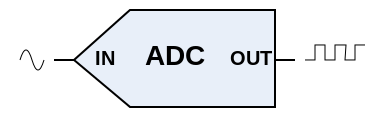
\includegraphics[width=.5\textwidth]{images/diagrama-adc.png}
	\caption[Diagrama funcional y símbolo eléctrico de un ADC]{Diagrama funcional y símbolo eléctrico de un ADC (tomada de \cite{WikiADC})}
	\label{F-diagrama-adc}
\end{figure}

Este proceso se basa en 2 subprocesos: muestreo, discretización temporal, y cuantización, discretización de la amplitud \cite{Proakis1996}. El muestreo puede ser visto como el parpadeo continuo de una persona, en el cual sólo se toma una imagen cada vez que se abren los ojos, la cantidad de veces que se abran por segundo se denominará frecuencia de muestreo (Fs); de tal manera al tomar una señal y muestrearla a cierta frecuencia, se tomará la amplitud de dicha señal cada vez que se tome un dato, dando como resultado una señal discretizada en el tiempo \cite{Prandoni2008}, la \figura{F-sampling} muestra un ejemplo de ello. \\

\begin{figure}[h!]
	\centering
	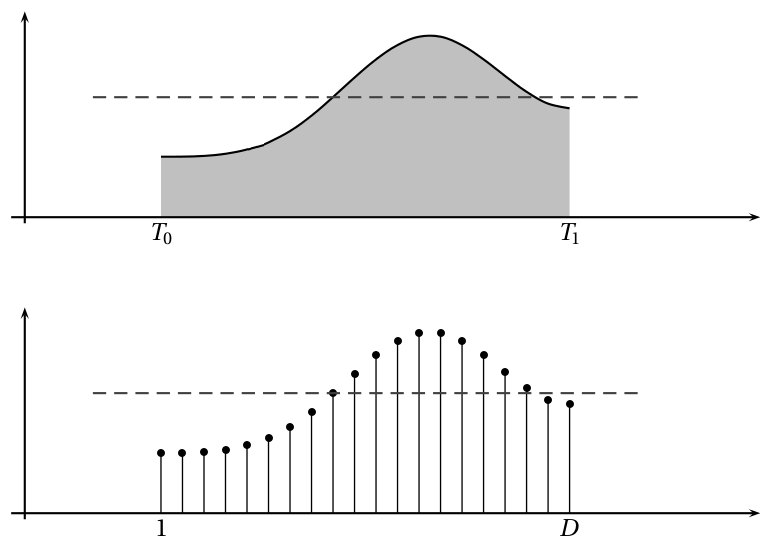
\includegraphics[width=.6\textwidth]{images/sampling.png}
	\caption[Muestreo de una señal]{Muestreo de una señal (tomada de \cite{Prandoni2008})}
	\label{F-sampling}
\end{figure}

Luego de tener una señal muestreada es necesario cuantizarla con el fin de discretizar sus amplitudes, esto es realizado al aplicar la \ecuacion{E-adc} a cada dato muestreado; en ella, $D$ es la salida digital, $n$ es la resolución, $V_{in}$ es el voltaje analógico de entrada, $V_{FSR}$ es el voltaje máximo. La resolución de un ADC representa el número de estados posibles, representados por $2^{n}$ pues es información digital en bits, de la salida digital \cite{AnalogDevices2005}. Este proceso añade un error a la señal digital, llamado error de cuantización, con un tamaño máximo de $\frac{1}{2}LSB$\nomenclature{LSB}{Bit menos significativo, por sus siglas en inglés}, una media de cero y una desviación estandar de $~0.29LSB$ \cite{Rodriguez2012}, en la \tabla{T-adc-error-c} se muestra una comparación entre resolución y error de cuantización.
\begin{equation}
	D = \frac{2^{n} \times V_{in}}{V_{FSR}}
	\label{E-adc}
\end{equation}
\begin{table}[H]
	\begin{center}
%		\resizebox{\textwidth}{!}{
			\begin{tabular}{|c|c|c|}
%			\begin{tabular}{|>{\centering\arraybackslash}m{2cm}| >{\centering\arraybackslash}m{5cm}| >{\centering\arraybackslash}m{5cm}|}
				\hline
				\textbf{Resolución (bits)} & \textbf{Ruido rms agregado a la señal} & \textbf{Valor de escala completa} \\ \hline
				8 & $\frac{0.29}{256}$ & $\frac{1}{900}$ \\ \hline
				12 & $\frac{0.29}{4096}$ & $\frac{1}{14000}$ \\ \hline
				16 & $\frac{0.29}{65536}$ & $\frac{1}{227000}$ \\ \hline
			\end{tabular}
%		}
	\caption{Error de cuantización}
	\label{T-adc-error-c}
	\end{center}
\end{table}

\textbf{Teorema de muestro.}
También llamado teorema de Nyquist, criterio de Nyquist o Teorema de muestreo de Nyquist-Shannon. Rodriguez \cite{Rodriguez2012} lo enuncia como que una señal continua puede ser adecuadamente muestreada sólo si no contiene componentes de frecuencia superiores a la mitad de la tasa de muestreo, o en las palabras del mismo Shannon \cite{Shannon1949}, \textit{``If a function $x(t)$ contains no frequencies higher than $B$ hertz, it is completely determined by giving its ordinates at a series of points spaced $\frac{1}{2B}$ seconds apart''}; esto matemáticamente se expresa en la \ecuacion{E-nyquist}, donde $F_{max}$ es la frecuencia máxima de la señal y Fs es la frecuencia de muestreo. De esta manera se denomina frecuencia de Nyquist \nomenclature{FN}{Frecuencia de Nyquist} a la máxima tasa que se puede alcanzar con una Fs determinada.
\begin{equation}
	Fs > 2F_{max}
	\label{E-nyquist}
\end{equation}

Basado en el comportamiento del fenómeno físico, en la intensidad del sonido y su relación con los seres humanos (\figura{F-intensidad}), y en el contexto planteado en las telecomunicaciones, se concluyó que una Fs de 8kHz es suficiente para abarcar el fenómeno físico.
\begin{figure}[h!]
	\centering
	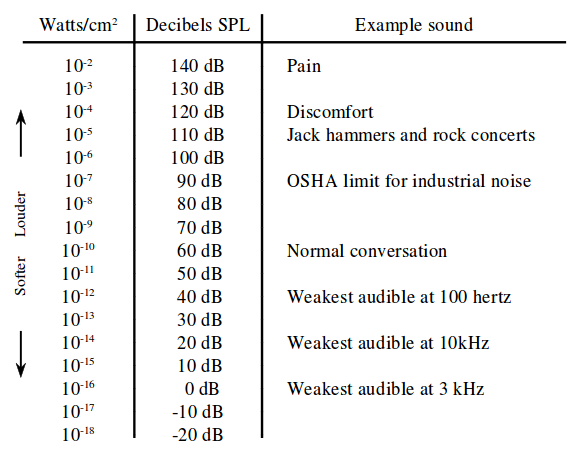
\includegraphics[width=.6\textwidth]{images/intensidad-audio.png}
	\caption[Unidades de intensidad de sonido]{Unidades de intensidad de sonido (tomada de \cite{Smith1997})}
	\label{F-intensidad}
\end{figure}

%Que me llevó a estas decisión
%A/D
%Analisis de Fourier (lo que me llevo a A/D)
%  NO ENTIENDO
%  FFT
%  analisis de audio
%INFOS
%Convertidor A/D


\subsection{Fase 2: Almacenamiento}
Luego de realizar la ditalización y contar con una señal que el procesador pueda manejar, se requiere grabarla o almacenarla; para ello se puede utilizar la memoria de cada dispositivo. El tiempo de grabación escogido se basó en los resultados obtenidos por Pell y Kotz \cite{Pell2011}, los cuales se presentan en la \figura{F-time-emotion}, allí se puede observar los tiempos necesarios para que una persona identifique una emoción. En el proyecto se tomaron tiempos de grabación de 2 a 4.5 segundos (cada 0.5 segundos), de modo que se tuviese tiempo suficiente para la expresión de la emoción y además permitir al usuario realizar variaciones dependiendo la situación.
\begin{figure}[h!]
	\centering
	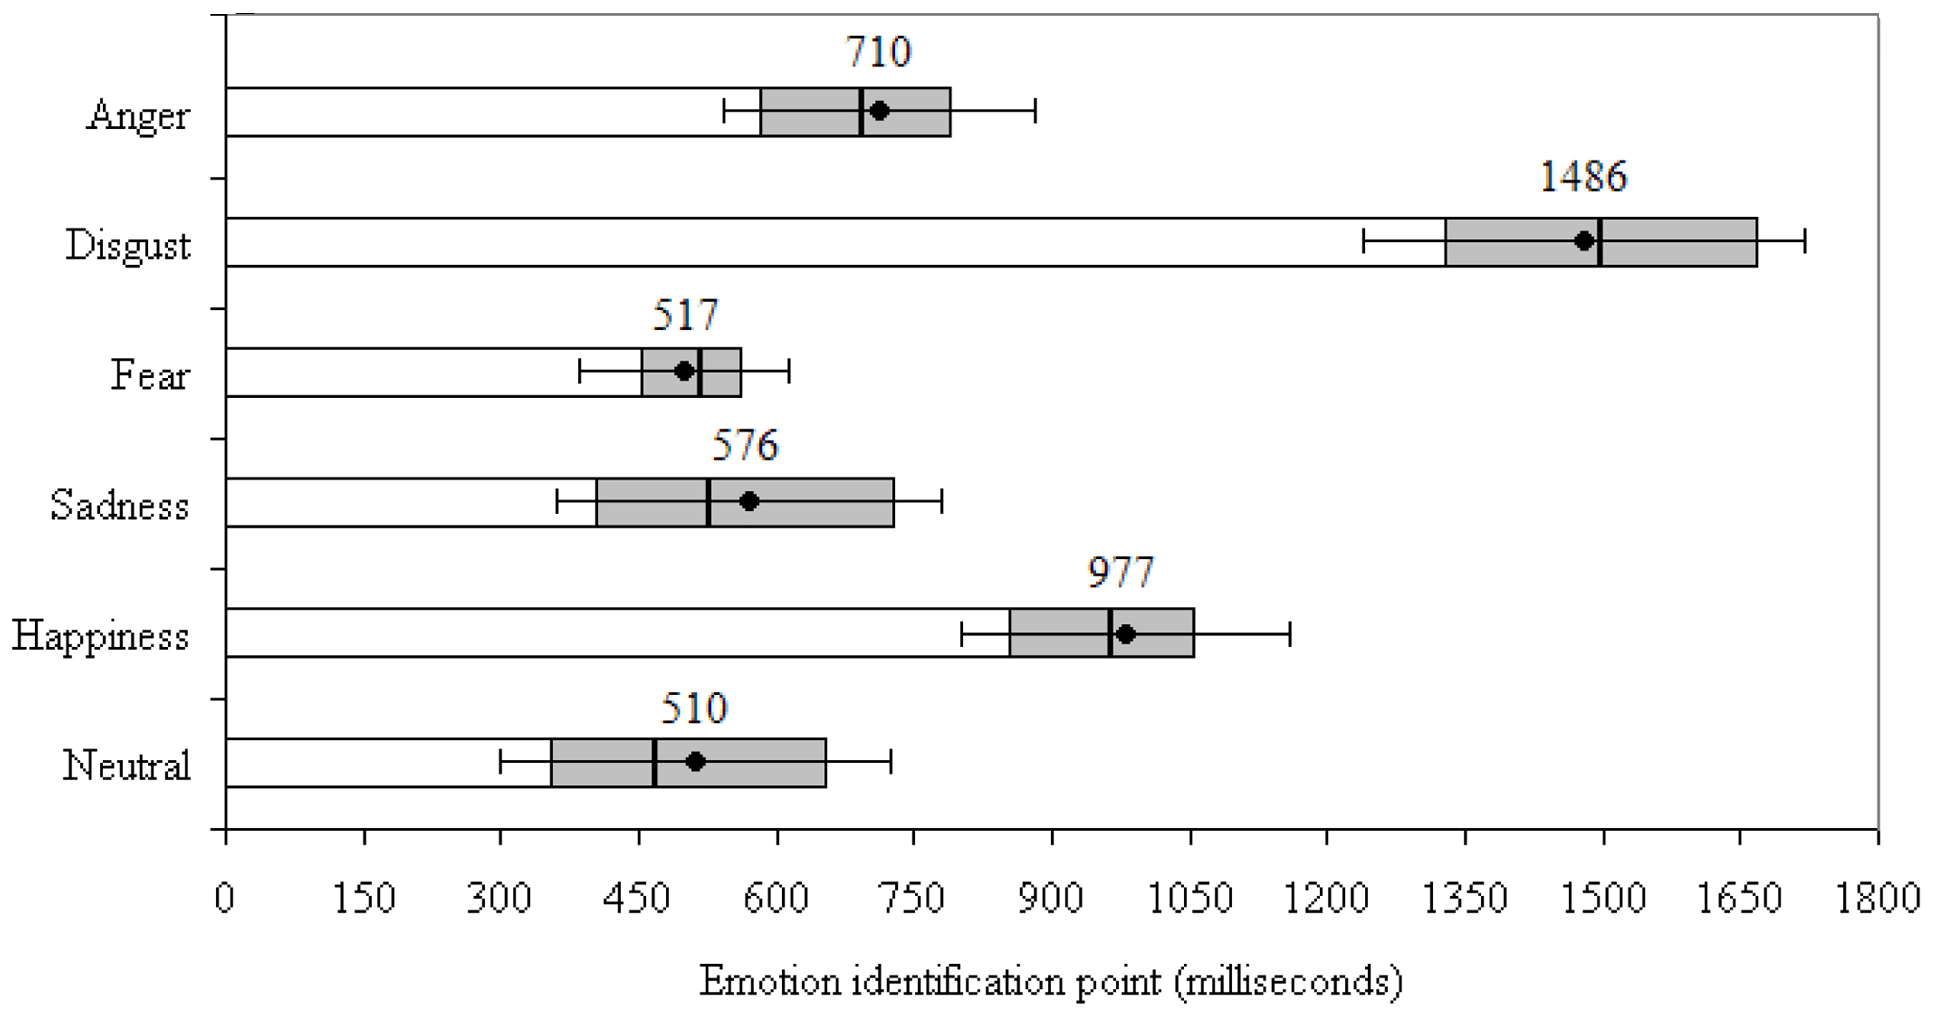
\includegraphics[width=.9\textwidth]{images/time-emotion.png}
	\caption[Tiempos de reconocimiento para diferentes emociones]{Tiempos de reconocimiento para diferentes emociones (tomada de \cite{Pell2011})}
	\label{F-time-emotion}
\end{figure}

%tiempos PAPER


\subsection{Fase 3: Filtrado de la señal}
Se puede definir un filtro como procedimientos donde se almacena y se manipula matemáticamente las muestras numéricas de tal forma que se pueda adquirir ciertas características específicas de la señal original. Un filtro se puede describir en forma de algoritmo, y en el caso de sistemas invariantes en el tiempo, como una ecuación en diferencias de coeficientes constantes \cite{Prandoni2008}.\\

\textbf{Sistemas lineales invariantes en el tiempo.}
Un filtro se puede definir como un sistema de una entrada y una salida, lineal y discreto en el tiempo. Desde otro punto de vista, se puede ver como un operador que transforma la señal de entrada en una salida deseada.
\begin{equation}
	y[n] = H\{x[n]\}
\end{equation}
Teniendo en cuenta que es un operador lineal, se cumple que:
\begin{equation}
	H\{\alpha x_{1}[n] + \beta x_{2}[n]\} = H\{\alpha x_{1}[n]\} + H\{\beta x_{2}[n]\}
\end{equation}
Al ser invariante en el tiempo se tiene:
\begin{equation}
	y[n] = H\{x[n]\} \Longleftrightarrow y[n-n_{0}] = H\{x[n-n_{0}]\}
\end{equation}
Esto significa que el sistema será igual en cualquier instante de tiempo y su salida no se ve afectada. Un sistema lineal invariante en el tiempo se caracteriza completamente por su respuesta al impulso. Para ver esto, una secuencia se puede escribir en su forma canónica orto normal como:
\begin{equation}
	x[n] = \sum_{k=-\infty}^{\infty} x[k]\delta[n-k]
\end{equation}
Teniendo en cuenta que $H\{\delta[n]\} = h[n]$, un filtro se puede escribir como:
\begin{equation}
	y[n] = H\{x[n]\} =  \sum_{k=-\infty}^{\infty} x[k]h[n-k]
	\label{E-conv-sec}
\end{equation}
La \ecuacion{E-conv-sec} se conoce como convolución de las secuencias $x[n]$ y $h[n]$.

\textbf{Filtros FIR.}
Teniendo en cuenta que los filtros son sistemas descritos completamente por su repuesta al impulso, un filtro FIR, es un tipo de filtro digital cuya respuesta a una señal impulso como entrada, tendrá como salida un numero finito de términos no nulos. La salida de este filtro sólo se basa en las entradas actuales y anteriores.
\begin{equation}
	y[n] = \sum_{k=0}^{N-1} b_{k} x[n-k]
	\label{E-filter-FIR}
\end{equation}
En la \ecuacion{E-filter-FIR}, N es el orden del filtro e indica el número de términos no nulos y de coeficientes. La salida también puede expresarse como la convolución de la señal de entrada $x[n]$
con la respuesta al impulso $h[n]$
\begin{equation}
	y[n] = \sum_{k=0}^{N-1} x[k] h[n-k]
\end{equation}
En la \figura{F-FIR} se presenta la estructura básica de un filtro FIR.
\begin{figure}[h!]
	\centering
	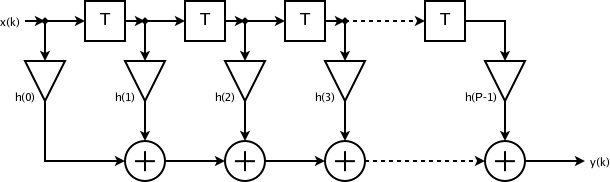
\includegraphics[width=1\textwidth]{images/FIR.png}
	\caption[Estructura de un filtro FIR]{Estructura de un filtro FIR (tomada de \cite{WikiFIR})}
	\label{F-FIR}
\end{figure}

\textbf{Filtros IIR.}
Consiste en un tipo de filtro digital en el que la respuesta a la entrada de una señal impulso, la salida tendrá un número infinito de términos no nulos, en este caso, el sistema nunca regresa al
reposo. La salida de los Filtros IIR depende tanto de las entradas pasadas y actuales como de las salidas anteriores. Matemáticamente se puede expresar el filtro IIR como:
\begin{equation}
	y[n] = b_{0}x[n] + \cdots + b_{N}x[n-N] - a_{1}y[n-1] - \cdots - a_{M}y[n-M]
\end{equation}
Donde a y b son los coeficientes del filtro y el orden es el máximo entre M y N. En la \figura{F-IIR} se presenta la estructura básica de un filtro IIR.
\begin{figure}[h!]
	\centering
	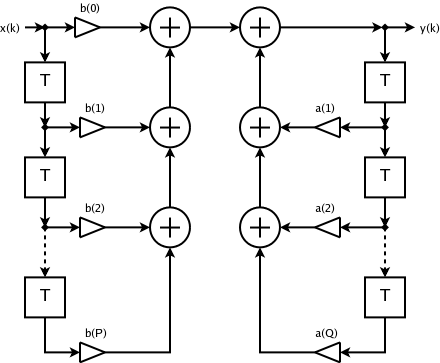
\includegraphics[width=.8\textwidth]{images/IIR.png}
	\caption[Estructura de un filtro IIR]{Estructura de un filtro IIR (tomada de \cite{WikiIIR})}
	\label{F-IIR}
\end{figure}

En la \tabla{T-FIR-IIR} se muestra una comparación entre filtros IIR y FIR.
\begin{table}[H]
	\begin{center}
		\resizebox{\textwidth}{!}{
			\begin{tabular}{|c||c|c|}
				\hline
				& \textbf{FIR} & \textbf{IIR} \\ \hline\hline
				\multirow{4}{*}{\textbf{Ventajas}} & Estabilidad incondicional & Bajo costo computacional \\ \cline{2-3}
& Cambio de fase lineal & Retraso entrada-salida corto \\ \cline{2-3}
& Procedimientos de diseño óptimos & Representación compacta \\ \cline{2-3}
& Robusto con respecto a la precisión finita numérica & - \\ \hline\hline
				\multirow{4}{*}{\textbf{Desventajas}} & Gran retraso entre entrada-salida & No se garantiza estabilidad \\ \cline{2-3}
				& Alto costo computacional & Respuesta de fase difícil de controlar \\ \cline{2-3}
				& - & El diseño es complejo en algunos casos \\ \cline{2-3}
				& - & Sensible a la precisión numérica \\ \hline
			\end{tabular}
		}
	\caption{Comparación entre filtros FIR e IIR}
	\label{T-FIR-IIR}
	\end{center}
\end{table}

\textbf{Transformada Z.}
Esta transformada realiza un mapeo entre secuencias complejas y funciones analíticas en el plano complejo. Se define como:
\begin{equation}
	X(z) = Z\{x[n]\} = \sum_{n=-\infty}^{\infty} x[n] z^{-n}
\end{equation}
Esta transformada es una herramienta fundamental en el procesamiento de señales, es muy útil para la solución de ecuaciones en diferencias con coeficientes constantes y además está asociada a la DTFT\nomenclature{DTFT}{Discrete Time Fourier Transform}, provee de criterios de estabilidad para el diseño de filtros digitales. La \ecuacion{E-Z-FIR} presenta la transformada Z para un filtro FIR y la \ecuacion{E-Z-IIR} para uno IIR.
\begin{equation}
	H(z) = \sum_{k=0}^{N-1} h[k] z^{-k}
	\label{E-Z-FIR}
\end{equation}
\begin{equation}
	H(z) = \dfrac{\sum_{k=0}^{N} b_{k} z^{-k}}{1 + \sum_{k=1}^{M} a_{k} z^{-k}}
	\label{E-Z-IIR}
\end{equation}

\textbf{Ecuaciones en diferencias de coeficientes constantes.}
Esta implica una relación directa entre la entrada y la salida.
\begin{equation}
	\sum_{k=0}^{N-1} a_{k} y[n-k] = \sum_{k=0}^{M-1} b_{k} x[n-k]
\end{equation}
Con $a_{0} = 1$ se obtiene:
\begin{equation}
	y[n] = \sum_{k=0}^{M-1} b_{k} x[n-k] - \sum_{k=1}^{N-1} a_{k} y[n-k]
\end{equation}


%INFOS


\subsection{Fase 4: Generación de gráficas}
Se considera importante contar con información adicional acerca de la señal de audio adquirida, por ello, en esta fase se generan las gráficas de la señal en el tiempo y su distribución de potencia. En la \figura{F-tspectrum} se muestra una señal de audio adquirida y su comportamiento en el tiempo, en la \figura{F-pspectrum} se presenta su periodograma, el cual representa la distribución de potencia de la señal.
\begin{figure}[h!]
	\centering
	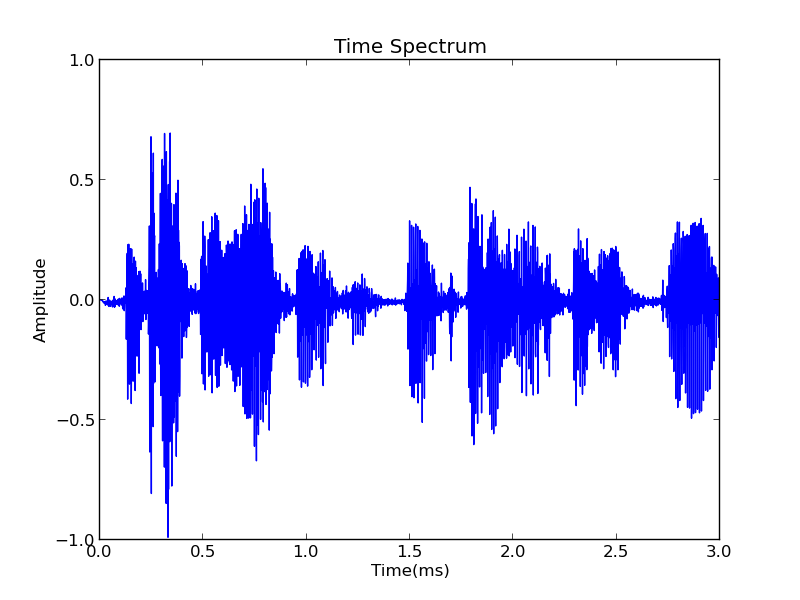
\includegraphics[width=.8\textwidth]{images/tspectrum.png}
	\caption{Señal de audio capturada}
	\label{F-tspectrum}
\end{figure}
\begin{figure}[h!]
	\centering
	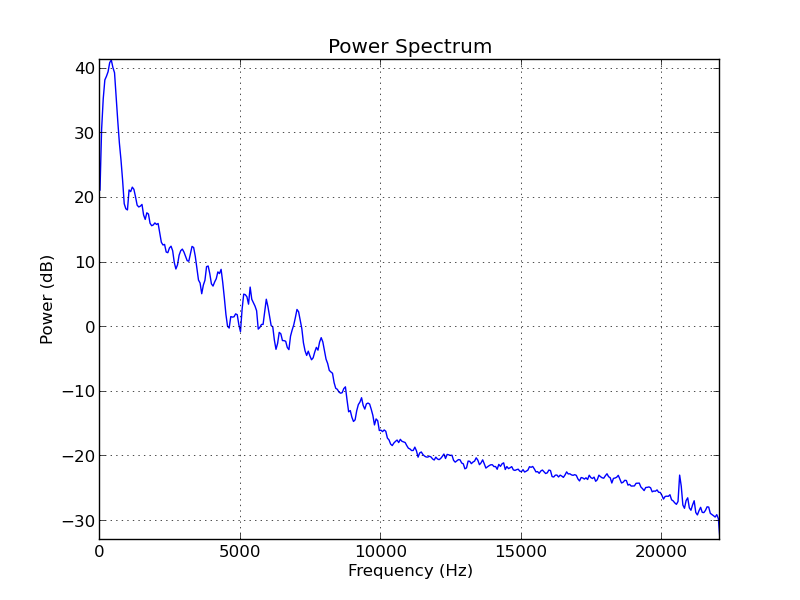
\includegraphics[width=.8\textwidth]{images/pspectrum.png}
	\caption{Periodograma de la señal de audio capturada}
	\label{F-pspectrum}
\end{figure}

%tiempo y frecuencia
%MIO


\subsection{Fase 5: Análisis wavelet}
%Burrus1997

En esta fase, el dispositivo realiza las transformadas wavelet con el nivel de resolución deseado por el usuario, a continuación se presentala teoría principal de dicha transformada, basadose en el trabajo presentado por Sripathi \cite{Sripathi2003}\\

La transformación de una señal es sólo otra forma de representar la señal. No cambia la información contenida en la señal. En cuanto a la transformación wavelet, ésta provee una representación temporal y frecuencial de la señal y fue desarrollada para superar a la transformada de tiempo corto de Fourier (STFT\nomenclature{STFT}{Short time Fourier transform}), la cual también puede ser usada para analizar señales no estacionarias. Mientras la STFT da una resolución constante en todas las frecuencias, la transformada wavelet usa la técnica multi-resolución en la cual diferentes frecuencias son analizadas con diferentes resoluciones. Una onda es una oscilación de tiempo o espacio y es periódica. Ahora bien, las wavelets son ondas localizadas y son aptas para el análisis de funciones trascendentes. Además, la STFT usa ondas para analizar señales, la transformada wavelet usa wavelets con energía finita. En la \figura{F-onda-wavelet} se presentan las gráficas características de una onda y un wavelet. \cite{Burrus1997}
\begin{figure}[h!]
	\centering
	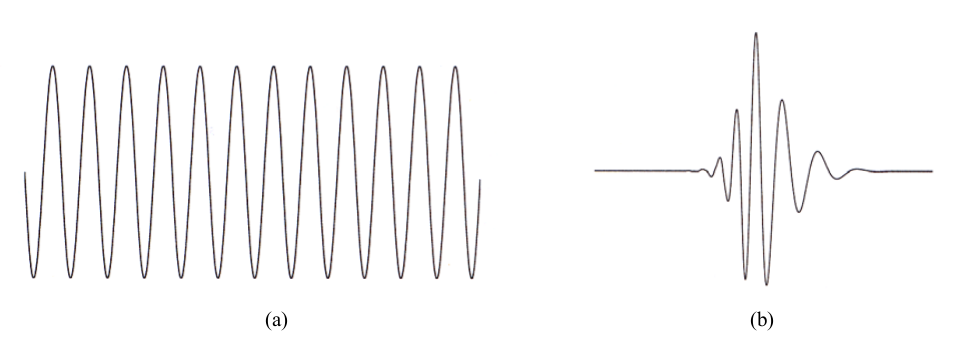
\includegraphics[width=.8\textwidth]{images/onda-wavelet.png}
	\caption[Representación de una onda y un wavelet]{Representación de una onda y un wavelet (tomada de \cite{Burrus1997})}
	\label{F-onda-wavelet}
\end{figure}

El análisis wavelet es similar al análisis de la STFT. La señal a ser analizada es multiplicada por una función wavelet tal y como se multiplica por una función ventana en la STFT, en la transformada wavelet, el ancho de la función wavelet cambia con cada componente espectral. La transformada wavelet, en altas frecuencias, da una buena resolución en tiempo y una pobre resolución en frecuencia, mientras que en bajas frecuencias, la transformada wavelet da una buena resolución en frecuencia y una pobre resolución en tiempo.\\

\textbf{La transformada wavelet continua y la serie wavelet.}
La transformada wavelet continua (CWT\nomenclature{CWT}{Transformada wavelet continua, por sus siglas en inglés}) está definida como se puede observar en la \ecuacion{E-wt}, donde $x(t)$ es la señal a ser analizada. $\psi(t)$ es la wavelet madre o la función base. Todas las funciones wavelet usadas en la transformaciones son derivadas de la wavelet madre a través de una translación (movimiento de fase) y escalamiento (dilatación o compresión).
\begin{equation}
	X_{wt}(\tau,s) = \dfrac{1}{\sqrt{|s|}}\int x(t)\cdot\psi^{*}\left(\dfrac{t-\tau}{s}\right) dt
	\label{E-wt}
\end{equation}

La wavelet madre usada para generar las funciones base, es diseñada pensando en algunas características deseadas asociadas con esa función. El parámetro de la translación $\tau$ está asociado con la localización de la función wavelet y con el desfase a lo largo de la señal. El parámetro de escala $s$ es definido como $\frac{1}{frecuencia}$ y corresponde a la información de la frecuencia. Escalando mediante la dilatación (expansión) o la compresión de una señal. Grandes escalas (bajas frecuencias) dilatan la señal y proporcionan información detallada que está escondida en la señal, mientras que las escalas pequeñas (altas frecuencias) comprimen la señal y dan información global acerca de la señal. Nótese que la compresión de la transformada wavelet simplemente lleva a cabo la operación de convolución de la señal y la función de base. El análisis anterior se vuelve muy útil en aplicaciones prácticas, las altas frecuencias (bajas escalas) no tienen una alta duración, en vez de ello, son como ráfagas cortas, mientras que las bajas frecuencias usualmente duran el tiempo total de la señal.\\

La serie wavelet es obtenida por la discretización de la CWT. Esto ayuda en el cálculo de la CWT mediante el uso de computadoras y se obtiene usando el muestreo del plano de escala de tiempo. La rata de muestreo pueda ser modificada de acuerdo con el cambio de la escala sin violar el criterio de Nyquist, expuesto anteriormente. Por tanto, si la escala va creciendo (frecuencias más bajas), la frecuencia de muestreo se puede disminuir reduciendo así el número de cálculos.\\

\textbf{Transformada wavelet discreta (DWT\nomenclature{DWT}{Transformada wavelet discreta, por sus siglas en inglés}).}
La serie wavelet es una versión muestreada de la CWT y su computo puede consumir tiempos y recursos elevados, dependiendo de la resolución requerida. La DWT está basada en una codificación sub-banda y se encuentra para producir un cómputo veloz de la transformada wavelet. Es fácil de implementar y reduce el tiempo de cómputo y los recursos necesarios, pues tiene una complejidad algorítmica lineal \cite{Rioul1992}.\\

Los fundamentos de la DWT se remontan a los años 1976, cuando las técnicas para la descomposición discreta de señales de tiempo fueron inventadas. Un trabajo similar fue realizado en la codificación de una señal de audio la cual fue llamada codificación sub-banda. En 1983, una técnica similar a la codificación sub-banda fue desarrollada, la cual fue llamada código piramidal. Más tarde, se hicieron muchas mejoras a estos sistemas de codificación que dieron lugar a esquemas eficientes de análisis multiresolución.\\

En la CWT, las señales son analizadas usando un conjunto de funciones bases que se relacionan unas con otras por un simple escalamiento y una translación. En este caso de DWT, una representación en la escala temporal de la señal digital es obtenida usando técnicas de filtrado digital. La señal a ser analizada es pasa a través de filtros con diferentes frecuencias de cortes en diferentes escalas.\\

\textbf{DWT y bancos de filtros.}\\
\textit{Análisis Multi-Resolución usando bancos de filtros.}
Las funciones wavelets pueden ser realizadas por la iteración de filtros con re-escalamiento. La resolución de la señal, la cual es una medida de la cantidad de información de detalle en la señal, es determinada por las operaciones de filtrado, y la escala es determinada por las operaciones de sobre-muestreo [upsampling] y disminución de resolución [downsampling] (subsampling).\\

La DWT es computada mediante filtrados pasa bajas y pasa altas del dominio de tiempo discreto de la señal tal y como se muestra en la \figura{F-desc-3}. Esto es llamado el algoritmo de Mallat o el árbol de descomposición de Mallat \cite{Sripathi2003}. Su importancia está en la forma que éste conecta la multi-resolución de tiempo continuo con los filtros de tiempo discreto. En la figura, la señal es denotada por la secuencia $x[n]$, donde $n$ es un entero. El filtro pasa bajas es denotado por $G_0$ mientras que las altas frecuencias están denotadas por $H_0$ . En cada nivel, el filtro pasa alto produce información de detalle, $d[n]$, mientras que el filtro pasa bajas asociado con el escalamiento de la función produce
aproximaciones gruesas, $a[n]$.
\begin{figure}[h!]
	\centering
	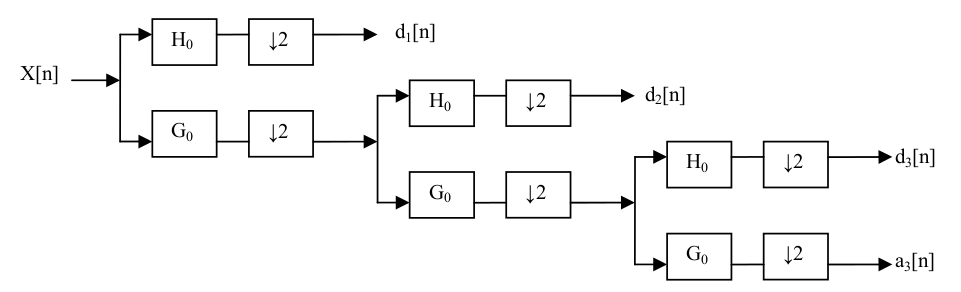
\includegraphics[width=.9\textwidth]{images/desc-3.png}
	\caption[Árbol de descomposición wavelet de 3 niveles]{Árbol de descomposición wavelet de 3 niveles (tomada de \cite{Sripathi2003})}
	\label{F-desc-3}
\end{figure}

En cada nivel de descomposición, los filtros de banda media producen señales que abarcan sólo la mitad de la banda de frecuencia. Esto dobla la frecuencia de resolución y la incertidumbre en frecuencia es reducida a la mitad y por esta razón se puede usar la mitad Fs inicial sin pérdida de información. Esta descomposición por 2 mitades de la resolución de tiempo hace que la totalidad de la señal sea ahora representada por sólo la mitad del número de muestras. Así, mientras que la banda media de filtrado paso bajo elimina la mitad de las frecuencias y por lo tanto reduce a la mitad la resolución, la descomposición por 2 duplica la escala.\\

Con este enfoque, la resolución temporal es mejor en las altas frecuencias, mientras que la resolución en frecuencia es mejor a bajas frecuencias. El filtrado y el proceso de descomposición son continuados hasta que el nivel deseado sea alcanzado. El número máximo de niveles depende del largo de la señal. La DWT de la señal original es obtenida por la concatenación de todos los coeficientes, $a[n]$ y $d[n]$, empezando desde el último nivel de descomposición.
\begin{figure}[h!]
	\centering
	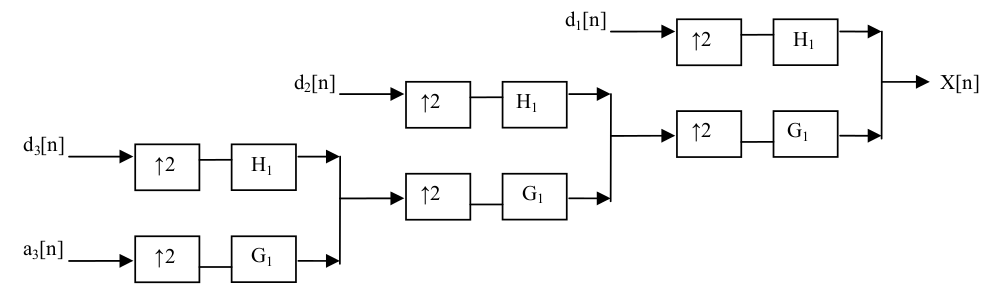
\includegraphics[width=.9\textwidth]{images/reco-3.png}
	\caption[Árbol de reconstrucción wavelet de 3 niveles]{Árbol de reconstrucción wavelet de 3 niveles (tomada de \cite{Sripathi2003})}
	\label{F-reco-3}
\end{figure}

La \figura{F-reco-3} muestra la reconstrucción de la señal original desde los coeficientes wavelet. Básicamente, la reconstrucción es el proceso inverso de descomposición. La aproximación y los coeficientes de detalle en cada nivel son muestreados por dos, se pasan a través de filtros pasa baja y pasa altas para luego ser sumados. Este proceso se continúa a través del mismo número de niveles que en el proceso de descomposición para obtener la señal original. El algoritmo de Mallat funciona igualmente bien si los filtros, $G_0$ y $H_0$ son intercambiados con los filtros $G_1$ y $H_1$.\\

\textit{Condiciones para una reconstrucción perfecta.}
En la mayoría de las aplicaciones de la transformada wavelet, se requiere que la señal original sea sintetizada desde los coeficientes wavelet. Para alcanzar la reconstrucción perfecta, los filtros de análisis y síntesis tienen que satisfacer ciertas condiciones. $G_0$ y $G_1$ deben ser de análisis pasa bajas y filtros de síntesis respectivamente. Entonces, los filtros tienen que satisfacer las condiciones de la \ecuacion{E-wavelet-cond}.
\begin{equation}
	\begin{aligned}
		G_0(-z)G_1(z) &+ H_0(-z)H_1(z) = 0 \\
		G_0(z)G_1(z) &+ H_0(z)H_1(z) = 2z^{-d}
		\label{E-wavelet-cond}
	\end{aligned}
\end{equation}

La primera condición implica que la reconstrucción está libre de \textit{aliasing} y la segunda condición implica que la amplitud de la distorsión tiene una amplitud de uno. Puede ser observado que la condición para la reconstrucción perfecta no cambia si se intercambian los filtros de análisis y síntesis. Hay un número de filtros que satisfacen estas condiciones. Pero no todos ellos dan una transformada wavelet precisa, especialmente cuando los coeficientes del filtro están cuantizados. La precisión de la transformada wavelet puede ser determinada después de la reconstrucción por el cálculo de la relación señal/ruido (SNR) de la señal. Algunas aplicaciones, como el reconocimiento de patrones no necesitan reconstrucción, y en tales aplicaciones, las condiciones
anteriores no necesitan aplicar.\\

\textit{Clasificación de wavelets.}
Se pueden clasificar las wavelets dentro de dos clases: ortogonales y biortogonales. Basado en la aplicación se puede utilizar una clase u otra. 
\begin{itemize}
	\item Características de los bancos de filtros wavelet ortogonales: 	Los coeficientes de los filtros ortogonales son números reales. Los filtros son del mismo tamaño y no son simétricos. El filtro pasa bajas $G_0$, y el filtro pasa altas $H_0$ están relacionados uno con el
otro por la \ecuacion{E-wavelet-rel-filter}
\begin{equation}
	H_0(z) = z^{-N}G_0(-z^{-1})
	\label{E-wavelet-rel-filter}
\end{equation}
	También, para la reconstrucción perfecta, los filtros de síntesis son idénticos a los filtros de análisis excepto por una inversión de tiempo. Los filtros ortogonales ofrecen un alto número de momentos de fuga. Esta propiedad es útil en muchas señales y en aplicaciones de procesamiento de imágenes. Ellos tienen estructuras regulares que propician fácil implementación y arquitectura escalable.
	\item Características de los bancos de filtros wavelet biortogonales: En este caso, los filtros pasa bajas y altas no tienen el mismo tamaño. Los filtros pasa bajas son siempre simétricos, mientras que los filtros pasa alta pueden ser simétricos o anti-simétricos. Los coeficientes de los filtros son números reales o enteros. Para la perfecta reconstrucción, los bancos de filtros biortogonales tienen todos tamaños pares. Los dos filtros de análisis pueden ser simétricos con tamaño par o uno simétrico y el otro anti-simétrico. También, los dos sets de análisis y filtros de síntesis deben ser duales. La fase lineal de los filtros biortogonales son los filtros más populares para aplicaciones de compresión de datos.\\
\end{itemize}

\textit{Familias de wavelet.}
Hay un número de funciones base que pueden ser usados como la wavelet madre para la transformación wavelet. Desde que la wavelet madre produzca todas las funciones wavelet usadas en la transformación a través de la translación y el escalamiento, eso determina las características del resultado de la transformada wavealiasinglet. Entonces, los detalles de la aplicación deberían ser tomados en cuenta y la wavelet madre apropiada debe ser escogida con el fin de usar la tranformada wavelet de manera efectiva.\\

La \figura{F-wavelet-ejem} muestra algunas de las funciones wavelet más comunes. Haar es una de las wavelet más antiguas y más simples, por ello cualquier discusión de wavelet empieza con ella. Daubechies\cite{Daubechies1992} son las wavelets más populares. Ellas representan las bases de procesamiento de señales wavelet y se utilizan en numerosas aplicaciones. Estas también son llamadas Maxflat wavelets ya que su respuesta en frecuencia tiene su nivel máximo de planitud en las frecuencias $0$ y $\pi$. Esto es una propiedad muy deseable en algunas aplicaciones. Las Haar, Daubechies, symlets y Coiflets son ortogonales y con soporte compacto. Estas wavelets junto con las wavelets Meyer permiten una reconstrucción perfecta. Las wavelets Meyer, Morlet y el sombrero mexicano son de forma simétrica. Las ondas se eligen en función de su forma y su capacidad para analizar la señal en una aplicación particular.
\begin{figure}[h!]
	\centering
	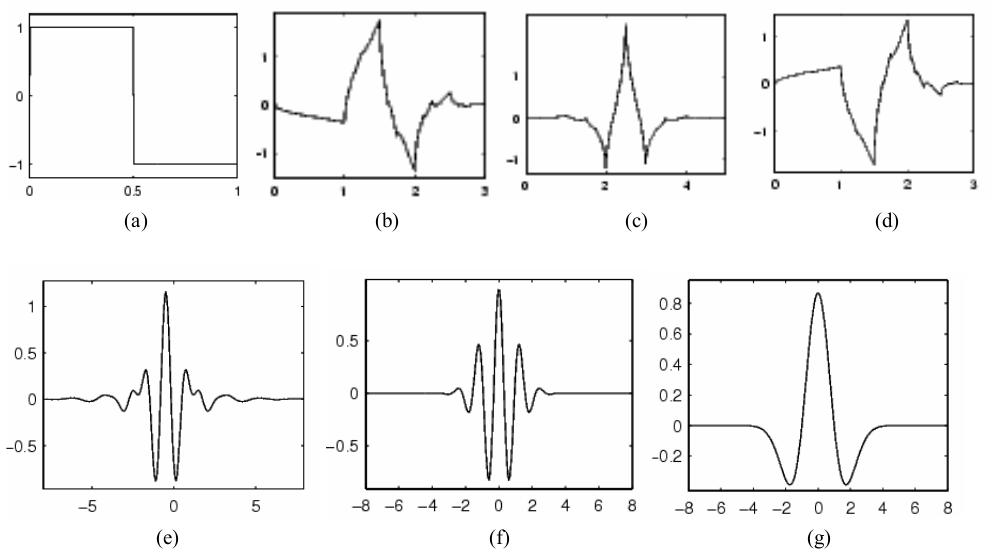
\includegraphics[width=.9\textwidth]{images/wavelet-ejem.png}
	\caption[Familias wavelet]{Familias wavelet: a)Haar b)Daubechies 4 c)Coiflet 1 d)Symlet 2 e) Meyer \mbox{f) Morlet} g) Sombrero mexicano  (tomada de \cite{Sripathi2003})}
	\label{F-wavelet-ejem}
\end{figure}

\textit{Aplicaciones.}
Hay un gran rango de aplicaciones en donde se usa la transformada wavelet. Ellas son aplicadas en diferentes campos que van desde el procesamiento de señales hasta la biometría, y esta lista está aun creciendo. Una de las aplicaciones más prominentes es en la compresión estándar de huellas digitales que hace el FBI. Las transformadas wavelet son usadas para comprimir las imágenes de las huellas digitales para ser almacenadas en bases de datos. La transformada discreta coseno (DCT\nomenclature{DCT}{Transformada discreta coseno, por sus siglas en inglés}) era anteriormente utilizada para este fin y no realizaba bien las altas compresiones. Esta producía gran cantidad de efectos de bloqueo que hacían imposible seguir las líneas rígidas de las huellas digitales después de la reconstrucción. Esto no pasa con la transformada wavelet debido a su propiedad de retener los detalle de los datos presentes.\\

En la DWT, la información más prominente en la señal aparece en las altas amplitudes y la información menos prominente aparece en las amplitudes más bajas. La compresión de datos puede ser alcanzada al descartar estas bajas amplitudes. La transformada wavelet permite altas compresiones y una buena calidad de reconstrucción. Actualmente, la aplicación de las wavelets para compresión de imágenes es una de las áreas más indagas en investigación. Recientemente, las transformadas wavelets han sido escogidas para la compresión estándar de JPEG 2000.
\begin{figure}[h!]
	\centering
	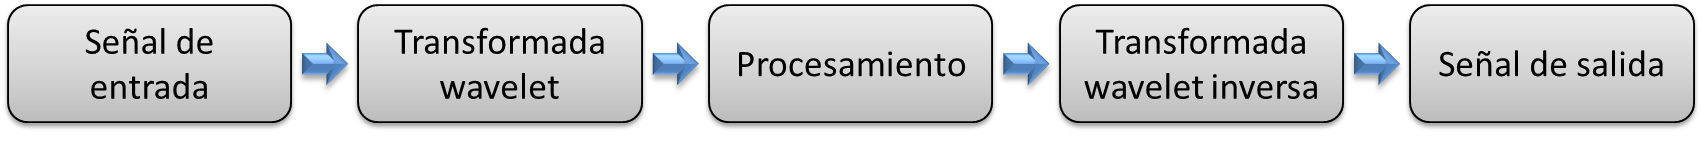
\includegraphics[width=.9\textwidth]{images/diagrama-wavelet.png}
	\caption{Procesamiento de señales con la transformada wavelet}
	\label{F-diagrama-wavele}
\end{figure}

La \figura{F-diagrama-wavele} muestra los pasos generales que se aplican en el procesamiento de señales. El procesamiento puede envolver compresiones, codificación, supresión de ruidos, entre otros. Las señales procesadas son almacenadas o transmitidas. Para la mayoría de las aplicaciones de compresión, el procesamiento envuelve cuantificación y codificación de entropía para producir una imagen comprimida. Durante este proceso, todos los coeficientes wavelet que están por debajo de un umbral escogido son descartados. Estos coeficietes descartados son reemplazados por ceros durante la reconstrucción. Para reconstruir la señal, la codificación de la entropía es decodificada, es cuantizada y finalmente se aplica la transformada wavelet inversa.\\

Las wavelets también tienen aplicación en la compresión de voz, lo cual reduce transmisión de tiempo en aplicaciones móviles. Ellas son usadas en supresión de ruidos, detección de cortes, extracción de características, reconocimiento de voz, cancelación de eco y otros. Esta técnica
promete mucho en aplicaciones de audio en tiempo real y en la compresión de videos. Las wavelet también tienen numerosas aplicaciones en comunicaciones digitales. \textit{Orthogonal Frequency Division Multiplexing} (OFDM\nomenclature{OFDM}{Orthogonal Frequency Division Multiplexing}) es una de dichas aplicaciones. Las wavelets son usadas en imágenes biomédicas. Por ejemplo, las señales de los electrocardiogramas, son analizadas usando wavelets o comprimidas para el almacenamiento. La popularidad de la transformada wavelet está creciendo debido a su capacidad de reducir la distorsión en la señal reconstruida, mientras retiene todas las características significantes presentes en la señal.

%INFOS


\subsection{Fase 6: Toma de decisiones}
\label{S-fase-6}
No se esperaba alcanzar esta fase en el desarrollo del proyecto de grado, pero sí es un objetivo a mediano plazo, por lo cual se propone como trabajo futuro (\seccion{S-trabajofuturo}), actualmente se tiene implementado un sistema de inferencia basado en lógica difusa que es capaz de distinguir alegría y tristeza.\\

\textbf{Lógica difusa.}
También llamada lógica borrosa o lógica heurística. Lofti A. Zadeh, profesor del Departamento de Ingeniería Eléctrica de la Universidad de California en Berkeley, a mediados de los 60's, publicó el artículo Fuzzy Sets \cite{Zadeh1965}. En este propuso una nueva lógica multi-valuada, retomando los conceptos expuestos anteriormente por lógicos como Lukasiewicz, Russell y Max Black. Zadeh, desarrolla un álgebra completa para conjuntos Borrosos, que resulta ser una extensión de la tradicional lógica bi-valuada (crisp), a la cual estamos acostumbrados. En la Lógica bi-valuada, no hay pertenencias parciales. Todo es exacto, sin incertidumbre; en cambio, en la lógica multivaluada (difusa) el razonamiento se fundamenta en conceptos lingüísticos, etiquetas verbales que califican el sistema tratado, como ``hace calor'', ``hace mucho calor''.

%TEX


\subsection{Selección final}
Se realizaron pruebas de funcionamiento sobre los materiales seleccionados en la propuesta de diseño (\seccion{S-prop-dise}); los elementos funcionaron sin problemas, excepto por el ADC click, pues no se logró una Fs adecuada para el fenómeno física abordado, por lo cual se utilizó el segundo componente con la mejor calificación de la fase de digitalización, la tarjeta de sonido USB. Por otra parte, inicialmente se pensaba utilizar un display gráfico como el uLCD-32PTU de 4D SYSTEMS \cite{SYSTEMS2013}
mostrado en la \figura{F-display-grafico}, en la mitad de la ejecución del proyecto se decidió utilizar en su lugar una pantalla HDMI\nomenclature{HDMI}{High-Definition Multimedia Interface} con el fin de reducir el tiempo de desarrollo y mejorar la visualización de las vistas. Estos cambios hicieron que la ruta final seguida en el proyecto fuese la expuesta en la \tabla{T-matriz-ruta-final}.
\begin{figure}[h!]
	\centering
	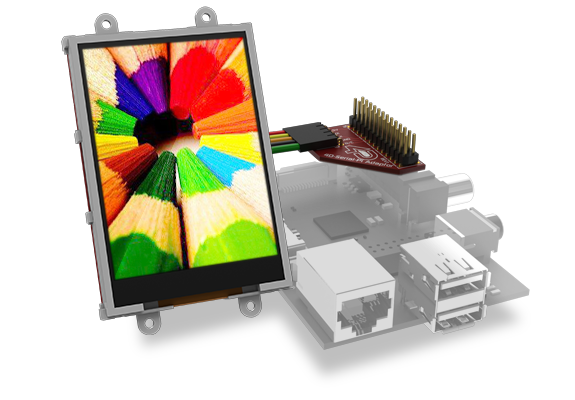
\includegraphics[width=.6\textwidth]{images/display-grafico.png}
	\caption[Display gráfico para Rpi]{Display gráfico para Rpi (tomado de \cite{SYSTEMS2013})}
	\label{F-display-grafico}
\end{figure}
\begin{table}[!h]
	\begin{center}
		\resizebox{\textwidth}{!}{
			\begin{tabular}{|c|c|ccccc|c|}
				\hline
				\multirow{2}{*}{\textbf{Periférico de entrada}} & \multicolumn{6}{c|}{\textbf{Fases}} & \multirow{2}{*}{\textbf{Periférico de salida}} \\ \cline{2-7}
%
%				& \textbf{Digitalización} & \multicolumn{1}{c|}{\textbf{Almacenamiento}} & \multicolumn{1}{c|}{\textbf{Filtrado de la señal}} & \multicolumn{1}{c|}{\textbf{Generación de gráficas}} & \multicolumn{1}{c|}{\textbf{Análisis wavelet}} & \multicolumn{1}{c|}{\textbf{Toma de decisiones}} & \\ \hline
				& \textbf{1} & \multicolumn{1}{c|}{\textbf{2}} & \multicolumn{1}{c|}{\textbf{3}} & \multicolumn{1}{c|}{\textbf{4}} & \multicolumn{1}{c|}{\textbf{5}} & \multicolumn{1}{c|}{\textbf{6}} & \\ \hline
%
				& \multirow{2}{*}{ADC Click} & \multicolumn{5}{c|}{FPGA} & \\ \cline{3-7}
%
				&& \multicolumn{5}{c|}{DSP} & \\ \cline{2-7}
%
				\multirow{3}{*}[13mm]{Armar el micrófono} & \multirow{2}{*}{Conversor Stereo A/D} & \multicolumn{5}{c|}{DSPic} & \multirow{3}{*}[13mm]{Display alfanumérico} \\ \cline{1-1} \cline{3-8}
%
				\cellcolor[gray]{0.7}&& \multicolumn{5}{c|}{\cellcolor[gray]{0.7}Raspberry Pi} & \cellcolor[gray]{0.7} \\ \cline{2-7}
%
				\cellcolor[gray]{0.7}& \cellcolor[gray]{0.7} & \multicolumn{5}{c|}{Arduino} & \cellcolor[gray]{0.7} \\ \cline{3-7}
%
				\cellcolor[gray]{0.7}\multirow{3}{*}[13mm]{Micrófono comercial} & \cellcolor[gray]{0.7}\multirow{2}{*}[7mm]{Tarjeta de sonido USB} & \multicolumn{5}{c|}{Microcontrolador} & \cellcolor[gray]{0.7}\multirow{3}{*}[13mm]{Display Gráfico (HDMI)}\\ \hline
			\end{tabular}
		}
	\caption{Ruta final de la matriz morfológica}
	\label{T-matriz-ruta-final}
	\end{center}
\end{table}

%Ruta final
%Las caracteristicas tecnicas se exponen en Hardware

%----------------- Revisión de Hardware (Capítulo) -------------------%
%Revisión de hardware
%- Micrófonos
%- ADC click (SPI)
%- Audio USB
%- Raspberry Pi

%curva del microfono

\cleardoublepage
\section{Hardware empleado}
\label{S-hardware}
En esta sección se muestran de manera más detallada las características de los elementos físicos principales utilizados en el proyecto.

\subsection{Fuente}
\label{S-fuente}
Para la conexión eléctrica se utilizó un toma corriente y una fuente de 5V\nomenclature{V}{Voltios} DC\nomenclature{DC}{Corriente directa, por sus siglas en inglés} a 2A\nomenclature{A}{Amperios}, con un salida USB\nomenclature{USB}{Universal Serial Bus} y protección de corto circuito, sus características se muestran en la \tabla{T-fuente}. La conexión del dispositivo final se expone en la \seccion{S-carac-elec}.
\begin{table}[H]
	\begin{center}
		%\resizebox{\textwidth}{!}{
		\begin{tabular}{|c|c|}
			\hline
			\multicolumn{2}{|c|}{Tablet Power Supply AD-2002U}\\ \hline
			Input voltage & AC\nomenclature{AC}{Corriente alterna, por sus siglas en inglés} 100V-240V 50/60Hz\nomenclature{Hz}{Hertz}\\ \hline
			Output voltage & DC 5V 2000mA\\ \hline
			Output port & 2xUSB type A female connector\\ \hline
			Protection & Short circuit protection\\ \hline
		\end{tabular}
		%}
	\end{center}
	\caption[Especificaciones técnicas de la fuente AD-2002U]{Especificaciones técnicas de la fuente AD-2002U, Techman Electronics Inc. (tomada de \cite{Techman})}
	\label{T-fuente}
%AD-2002U
%Tablet Power Supply
%	Specifications:
%- Input voltage: AC 100V-240V 50/60Hz
%- Output voltage: DC 5V 2000mA, 2xUSB type A female connector
%- Short circuit protection
%http://www.techman-usa.com/display.php?eC_type=DISPLAY&psid=AD-2002U&lang=en
%http://www.techman-usa.com/info/69-71.pdf
\end{table}

\subsection{Micrófono}
Las características del micrófono utilizado para la adquisición de la voz, se muestran en la \tabla{T-mic}, este se conecta directamente al puerto de entrada de la tarjeta de sonido USB.
\begin{table}[H]
	\begin{center}
		%\resizebox{\textwidth}{!}{
		\begin{tabular}{|c|c|}
			\hline
			\multicolumn{2}{|c|}{Micrófono Genius MIC-01A}\\ \hline
			Tipo & Omni-directional\\ \hline
			Impedancia de salida & 2.2k ohm (Max)\\ \hline
			Sensibilidad & -62dB +-4dB (a 1k Hz)\\ \hline
			Respuesta en frecuencia & 100Hz a 10k Hz\\ \hline
		\end{tabular}
		%}
	\end{center}
	\caption[Especificaciones técnicas del micrófono MIC-01A]{Especificaciones técnicas del micrófono, Genius MIC-01A (versión modificada de \cite{Genius2009})}
	\label{T-mic}
%http://www.geniusnet.com/wSite/ct?xItem=16664&ctNode=145
\end{table}
 
\subsection{ADC-Click}
Este fue el elemento escogido inicialmente por el diseño conceptual (\seccion{S-diseño}) como ADC\nomenclature{ADC}{Convertidor analógica digital, por sus siglas en inglés}, es un circuito que reúne diferentes integrados, de los cuales el principal es un MCP3204 y los demás se encargan de su configuración, las características principales se muestran en la \tabla{T-adc-click}. Lastimosamente al ser conectado al Rpi, por medio de SPI\nomenclature{SPI}{Serial Peripheral Interface}, no se lograron tazas mayores a 6ksps\nomenclature{ksps}{Kilo-muestras por segundo, por sus siglas en inglés}, lo que lo hizo inviable y fue reemplazado por el elemento con la segunda mejor calificación en el diseño conceptual, la tarjeta de sonido USB expuesta en la \seccion{S-audio-usb}.
%12-bit resolution
%4 (MCP3204) or 8 (MCP3208) input channels
%Analog inputs programmable as single-ended or
%pseudo-differential pairs
%On-chip sample and hold
%SPI serial interface (modes 0,0 and 1,1)
%Single supply operation: 2.7V
%50 ksps max. sampling rate at VDD = 2.7V
%Industrial temp range: -40°C to +85°C
\begin{table}[H]
	\begin{center}
		%\resizebox{\textwidth}{!}{
		\begin{tabular}{|c|c|}
			\hline
			\multicolumn{2}{|c|}{ADC-Click}\\ \hline
			Resolution & 12-bit \\ \hline
			Input channels & 4 \\ \hline
			Analog inputs programmable & Single-ended or pseudo-differential pairs \\ \hline
			Sample and hold & On-chip \\ \hline
			Communication interface & SPI \\ \hline
			Single supply operation & 2.7V \\ \hline
			Max. sampling rate & 50 ksps \\ \hline
			Industrial temp range & -40$^{\circ}$C to +85$^{\circ}$C \\ \hline
		\end{tabular}
		%}
	\end{center}
	\caption[Especificaciones técnicas del ADC-Click]{Especificaciones técnicas del ADC-Click, MikroElektronika (tomada de \cite{Microchip})}
	\label{T-adc-click}
%2.7V 4-Channel/8-Channel 12-Bit A/D Converters with SPITM Serial Interface
\end{table}

\subsection{Tarjeta de audio USB}
\label{S-audio-usb}
Este elemento es el segundo con la mejor calificación en el diseño conceptual (\seccion{S-diseño}) como ADC y fue utilizado debido a los problemas presentados con el ADC-Click. Cuenta con diversas frecuencias de muestreo, un canal de entrada y uno de salida, en el dispositivo sólo se utiliza el de entrada; además posee una interfaz USB con la cual se conecta al Rpi.
\begin{table}[H]
	\begin{center}
		%\resizebox{\textwidth}{!}{
		\begin{tabular}{|c|c|}
			\hline
			\multicolumn{2}{|c|}{Tarjeta de sonido USB}\\ \hline
			Conexión & USB\\ \hline
			Entrada de audio & \textit{Jack} de 3.5mm\\ \hline
			Salida de audio & \textit{Jack} de 3.5mm\\ \hline
			Resolución & 16-bit \\ \hline
			Frecuencias de muestreo (Hz) & 8000, 11025, 16000, 22050, 32000, 44100, 48000\\ \hline
		\end{tabular}
		%}
	\end{center}
	\caption[Especificaciones técnicas de la tarjeta de sonido 3D SOUND]{Especificaciones técnicas de la tarjeta de sonido 3D SOUND, Dynamode USB-SOUNDCARD2.0 (basada en \cite{Dynamode})}
	\label{T-audio-usb}
%http://www.dynamode.com/english/distributor.html
\end{table}

\subsection{Raspberry pi\textregistered\ (Rpi)}
%The Raspberry Pi is a credit-card sized computer that plugs into your TV and a keyboard. It’s a capable little PC which can be used for many of the things that your desktop PC does, like spreadsheets, word-processing and games. It also plays high-definition video. We want to see it being used by kids all over the world to learn programming.
Este dispositivo es un computador del tamaño de una tarjeta de crédito desarrollado por la \emph{Raspberry Pi Foundation} con la intención de promover el aprendizaje de la programación en niños alrededor del mundo \cite{Raspberry}. En el proyecto se utilizó como elemento de procesamiento y sus características se muestran en la \tabla{T-rpi}; para trabajar con él durante el desarrollo del proyecto se utilizó un televisor, un \textit{mouse} y un teclado.
\begin{table}[H]
	\begin{center}
		%\resizebox{\textwidth}{!}{
		\begin{tabular}{|c|c|}
			\hline
			\multicolumn{2}{|c|}{Raspberry pi\textregistered\ (Rpi)}\\ \hline
			Chip & Broadcom BCM2835 SoC full HD multimedia applications processor\\ \hline
			CPU & 700 MHz Low Power ARM1176JZ-F Applications Processor\\ \hline
			GPU & Dual Core VideoCore IV® Multimedia Co-Processor\\ \hline
			Memory & 512MB SDRAM\\ \hline
			Ethernet & 10/100 Ethernet RJ45 jack\\ \hline
			USB 2.0 & Dual USB Connector\\ \hline
			Video Output & HDMI, RCA\\ \hline
			Audio Output & 3.5mm jack, HDMI\\ \hline
			Low-level peripherals & \nomenclature{GPIO}{Entradas y salidas de propósito general, por sus siglas en inglés}General Purpose Input/Output (GPIO) pins, SPI, I$^2$C, I$^2$S, UART\\ \hline
			Onboard Storage & SD, MMC, SDIO card slot\\ \hline
			Operating System & Linux\\ \hline
			Dimensions & 8.6cm x 5.4cm x 1.7cm\\ \hline
		\end{tabular}
		%}
	\end{center}
	\caption[Especificaciones técnicas del Raspberry pi\textregistered\ (Rpi)]{Especificaciones técnicas del Raspberry pi\textregistered\ (Rpi), Raspberry Pi Foundation (tomada de \cite{ElinuxHardware})}
	\label{T-rpi}
%http://downloads.element14.com/raspberryPi1.html
%http://elinux.org/RPi_Hardware#Specifications
\end{table}

%----------------- Revisión de Software (Capítulo) -------------------%
\cleardoublepage
\section{Software empleado}
\label{S-software}
%Revisión de software
%- Rasbian
%- alsa
%- Python (g++)
%- scipy.io.wavfile (varias maneras de hacerlo)
%- numpy.fft
%- pywt (scipy.signal sunpy)
%- tkinter (Qt...)

Actualmente existen diferentes OS\nomenclature{OS}{Sistema operativo, por sus siglas en inglés} para el Rpi, entre los OS se encuentra:
\begin{itemize}[nolistsep]
	\item Raspbian
	\item OpenELEC
	\item Arch
	\item RaspBMC
	\item RISC OS
	\item Pidora
\end{itemize}
En este momento \emph{Raspberry Pi Foundation} recomienda instalar \textit{New Out of Box Software} (NOOBS), el cual es un conglomerado de OS entre los que se encuentran Raspbian y Pidora, así, la primera vez que se enciende el Rpi, el usuario debe escoger el OS a instalar \cite{Raspberry}. Por otra parte, el primer ampliamente difundido OS fue Rasbian, además tiene un buen soporte por parte de la fundación y cuenta con un amplio número de paquetes; por estas razones y por su similitud a Debian (Distribución popular de Linux, ver \href{http://www.debian.org}{www.debian.org}) se eligió como OS para el Rpi del proyecto. \\

Por la parte del desarrollo de software necesario en la herramienta se tenían diferentes alternativas. Como lenguaje de programación se consideró C++ y Python (\seccion{S-python}), un lenguaje copilado contra uno interpretado. Se conoce que el primero suele tener un tiempo de ejecución más corto, pero uno tiempo de desarrollo más largo, mientras que el segundo suele tener un tiempo más largo de ejecución, pero su desarrollo es más rápido. C++ es un lenguaje más antiguo, ampliamente difundido en las ciencias y con una gran cantidad de paquetes disponibles, por su parte, Python es un poco más nuevo, está ganando espacio en las ciencias y también cuenta con una gran cantidad de paquetes disponibles gracias a la comunidad que ha generado. Para el trabajo se prefirió Python principalmente debido al tiempo de desarrollo, pues este es un gran limitante en el desarrollo de este proyecto. Python, a pesar de ser un lenguaje multiparadigma, tiene una fuerte orientación a objetos, incluso en él todo es un objeto, por ello y por las ventajas que trae utilizar este paradigma de programación, se optó por utilizar POO\nomenclature{POO}{Programación Orientada a Objetos} (\seccion{S-POO}) dentro del proyecto aquí expuesto.\\

Para la construcción de la GUI se contaba de diferentes opciones como lo son Qt, GTK y Tk; pues Python cuenta con gran variedad de paquetes para este fin: PyQt, PyGtk, Tkinter (\seccion{S-tkinter}), entre otros; se eligió Tk debido a que Tkinter viene integrado con Python.\\

A pesar de que Python cuenta con paquetes para el manejo de periféricos, se seleccionó ALSA (\seccion{S-alsa}) para el manejo de las interfaces de audio y realizar la etapa de comunicación con el hardware por medio del OS, de manera de realizar la grabación de la señal de audio a analizar. Se escogió ALSA sobre los paquetes de Python, pues es robusto, cuenta con un buen soporte y está integrado por defecto en Rasbian; lo que hace que el proceso se pueda realizar independiente al programa desarrollado en Python, y así, este último puede correr independiente a la grabación, lo que podría facilitar la implementación en tiempo real propuesta en la sección de trabajo futuro (\seccion{S-trabajofuturo}). Por último, la \seccion{S-sw-des} habla sobre la implementación realizada en el proyecto, esta es la encargada de agrupar y utilizar las demás herramientas expuestas en esta sección.

\subsection{Rasbian}
%http://www.raspberrypi.org/downloads
%http://en.wikipedia.org/wiki/Raspberry_Pi#Raspbian
%http://elinux.org/RPi_Distributions#Raspbian
%http://elinux.org/Raspbian
%http://www.raspbian.org/

\begin{center}
	\textit{Raspberry Pi + Debian = Raspbian}\cite{ElinuxDistributions} %%http://elinux.org/RPi_Distributions#Raspbian
\end{center}

Como lo indica su página oficial \cite{Raspbian}: Raspbian es un OS libre, basado en Debian, con un entorno de escritorio LXDE y optimizado para el hardware del Rpi. No obstante, Raspbian provee más que un OS: él cuenta con más de 35.000 paquetes, pre-copilados en un formato para una fácil instalación en el Rpi. Además, aún se encuentra activamente en desarrollo, con énfasis en el mejoramiento, la estabilidad y el desempeño de la mayor cantidad de paquetes de Debian como sea posible.\\

Raspbian es desarrollado y mantenido por un grupo de desarrolladores admiradores del Rpi, las metas educacionales de la \emph{Raspberry Pi Foundation} y de Debian; pero estos no tiene ninguna afiliación a la fundación en si, por lo cual ella produce su propia imagen recomendada del OS \cite{Raspbian}, está disponible en la página oficial de Rpi (\href{http://www.raspberrypi.org/downloads}{www.raspberrypi.org/downloads}). Dicha imagen es instalada en una memoria SD con un tamaño mínimo 2GB, aunque se recomienda una de 4GB.

\subsection{Python}
\label{S-python}
%http://en.wikipedia.org/wiki/Python_%28programming_language%29
%http://www.learnpython.org/
%http://www.codecademy.com/tracks/python
%http://swaroopch.com/notes/python/
%http://www.python.org/
%
%Referencias:
%1. http://www.python.org/
%2. http://www.python.org/about/
%3. Byte of Python
%4. Python para todos
%5. http://en.wikipedia.org/wiki/Python_(programming_language)
%6. http://docs.python.org/2/library/
Python se define como un lenguaje de programación multiparadigma \cite{Python}, es decir que puede soportar diferentes formas de escritura de código, entre las cuales se encuentran paradigmas de programación imperativo, orientado a objetos, funcional, procedural, entre otros; esta característica permite al usuario tener cierta libertad sobre el desarrollo de su código de programación y adaptarlo a sus necesidades; a pesar de que Python soporte varios paradigmas es altamente encaminado a POO. \\

Una característica fundamental de Python es que se trata de un lenguaje interpretado y esto quiere decir que no necesita ser compilado a binario al ejecutarse como otros lenguajes, él mismo por medio de un intérprete traduce el código a una forma de pseudocódigo denominada bytecodes \cite{GonzalezPython}, traduce esto al idioma nativo del ordenador y luego ejecuta, lo cual simplifica el trabajo para quien programa, dado que no es necesario tener en cuenta cómo se va a compilar un código, Python lo hace por sí sólo y esto hace que se pueda ejecutar en cualquier computador, pero el código de un lenguaje interpretado se vuelve más lento dada la interpretación y traducción necesaria cada vez que se desea ejecutar a diferencia de los lenguajes compilados en donde este proceso sólo ocurre una vez, sin embargo un lenguaje interpretado es más flexible, portable y de rápido desarrollo. \\

Otro rasgo distintivo de este lenguaje es el tipado: Tipado dinámico y fuertemente tipado \cite{Swaroop2013}\cite{GonzalezPython}, el primero de ellos se refiere a como es la definición de variables, en síntesis no es necesario declarar de que tipo va a ser una variable, basta con asignarle un valor y éste se establecerá automáticamente, al cambiar el valor de la variable el tipo también se redefinirá. El segundo aspecto restringe el trato que se le da a las variables, es decir no es posible operar una variable con un tipo distinto al que tiene, por ejemplo no se puede tratar una variable que contiene texto como un número o viceversa. \\

Este lenguaje se enfoca en que su sintaxis sea simple, clara y transparente, tanto para quien escribe como para un lector, esto quiere decir que se pueden transmitir ordenes complejas con pocas líneas de código y con menos caracteres, si se compara con otros lenguajes; ejemplo de ello es una de sus características principales: La indentación, la cual consta de un espacio en blanco que delimita el comienzo de funciones o declaraciones, en lugar del uso de paréntesis o llaves, como es muy común en otro tipo de lenguajes, esto hace que la forma en que se escribe y se lee un código en Python sea más natural e intuitiva. \\

Además cuenta con la cualidad de ser un lenguaje desarrollado bajo la filosofía de código libre o abierto (Open Source), lo cual hace que el acceso a este, a librerías y paquetes de trabajo sea mucho más sencillo, compartido universalmente y no esté restringido a un único sistema operativo \cite{Python}. Y esa es precisamente uno de los aspectos más distinguidas del lenguaje: la amplia variedad de librerías y paquetes que posee, como funciones incorporadas, operaciones booleanas, procesamiento de texto, manejo de diferentes tipos de datos y archivos, módulos numéricos, matemáticos y científicos, herramientas de criptografía, acceso a directorios, compresión de datos, manipulación de datos en internet y módulos gráficos \cite{Pythonlibrary}, por nombrar algunos casos. Un aspecto importante, especialmente para los programadores, derivado también de su base de software libre, es la extensa comunidad que rodea a este lenguaje; Python cuenta con una documentación completa y detallada que provee la página oficial de este lenguaje, pero además de eso existen usuarios en todo el mundo que contribuyen a ampliar y difundir cada vez más el conocimiento acerca de Python de manera gratuita, en forma de conferencias, libros, repositorios, páginas web, tutoriales y ayudas de todo tipo \cite{Python}, lo cual tiene dos ventajas: para quienes son principiantes en el tema de programación en Python todas estas herramientas hacen que el aprendizaje sea más sencillo, amigable y rápido, y para quienes ya son programadores experimentados enriquece el lenguaje de programación y puede ser una ayuda en una situación específica.

\subsection{Programación Orientada a Objetos (POO)}
\label{S-POO}
%9. http://en.wikipedia.org/wiki/Object-oriented_programming
%10. http://es.wikipedia.org/wiki/Programaci%C3%B3n_orientada_a_objetos#Conceptos_fundamentales
%Scott, M. L.: Programming Language Pragmatics. Morgan Kaufmann Publishers, Elsevier, segunda edición, 2006.
%Van Roy, P. y S. Haridi: Concepts, Techniques, and Models of Computer Programming. MIT Press, 2004.

%Conceptos:
%Clase
%Atributos
%Métodos
%Objeto
%Identificador
%Estados
%Eventos
%Mensajes
%
%Características:
%Modularidad [Modular].
%Abstracción [Abstraction].
%Encapsulamiento [Encapsulation].
%Principio de ocultación [Hiding].
%Polimorfismo [polymorphism].
%  Sobrecarga
%  Dinámica y estática.
%Herencia [inheritance].
%Recolector de basura [Garbage collector].


Se define como un paradigma de programación a un estilo particular y aceptado por la comunidad de programación. En este caso la Programación Orientada a Objetos es uno de los tantos paradigmas existentes en la actualidad, que además se encuentra entre los más usados y difundidos mundialmente, siendo Smalltalk, Objective-C, Eiffel, C++, Java, C\#, Simula, Ada, Python, Ruby, entre otros los lenguajes que soportan este tipo de programación \cite{Scott2006}. \\

El eje central de este paradigma es el uso de entidades denominadas precisamente objetos, los cuales poseen atributos que los describen y están asociados a procedimientos, los cuales se denominan métodos; de esta forma un objeto dentro de este tipo de programación se puede asociar a un “objeto” en la vida real, el cual tiene características, realiza acciones o funciones e interactúa con otros objetos. Dentro de este paradigma se establecen conceptos principales que permiten entender su funcionamiento; el primero de ellos es la Clase, una clase consiste en la definición de las propiedades y comportamiento de un tipo de objeto, asociada a una clase existe una instanciación, la cual es básicamente la lectura de dichas definiciones y la creación de un objeto perteneciente a esa clase. También se define la Herencia, la cual consiste en la capacidad entre dos o más clases de heredar atributos y operaciones de otra clase, como si estuviesen definidos para ambas; lo cual permite usar métodos, atributos o funciones declarados en diferentes clases \cite{VanRoy2004}. Además uno de los conceptos principales es claramente los Objetos, los cuales son instancias de una clase, y como se señaló anteriormente poseen atributos y métodos, que definen sus características y funcionalidad; además cuentan con la característica de reaccionar a eventos, según sean los métodos y finalmente los métodos están definidos como un algoritmo en donde se ejecuta lo que el objeto está definido para hacer, un método puede causar cambios en las propiedades del objeto o generación de nuevos eventos.\\

Para ejemplificar todas las definiciones se puede pensar en asociar objetos de la vida real a ellas, como lo es un carro: en este caso el carro sería el objeto, el cual pertenece a una clase, en esta clase están contenidos todos los carros que tengan características o comportamiento similares; entonces se puede definir una clase llamada “Carros”, la cual tiene propiedades como “Marca” y “color” y tiene comportamientos definidos como “Carros deportivos”, por lo cual a esta clase pertenecerían los objetos llamados “Carro 1”, “Carro 2” y “Carro 3”, que tienen como atributos el color y la marca, además de ello un método que sería lo que pueden hacer, en este caso correr carreras, dado que son carros deportivos y finalmente si se quisiera crear una nueva clase llamada “Autos” se podría seleccionar que esta heredará de la clase “Carros” las propiedades de “Marca” y “Color” pero no el comportamiento “Carros deportivos”y así tendría objetos “Carro 4” y “Carro 5” que poseerían las mismas características “Marca” y “Color” que los objetos de la clase “Carros”, pero con comportamiento diferente.

\subsection{Paquetes científicos}
El significado de los ``paquetes'' en Python es similar al de las ``librerías'' en C++. Ahora, uno de los puntos más fuertes del lenguaje escogido es la disponibilidad de paquetes adicionales con la que cuenta,  actualmente son unos 36.304\cite{PythonIndex} y creciendo, pues estos le permiten extender sus habilidades. De esta manera, con paquetes como numpy, scipy o matplotlib, que brindan habilidades científicas al lenguaje, Python podría llegar a ser comparado con Matlab\textregistered\ en algunos aspectos, pues puede realizar tareas similares.\\

Con el fin de extender la comprensión de este trabajo para personas poco conocedoras de lo que significa un desarrollo en Python, el software generado en este proyecto podría ser comparado con una herramienta desarrollada en Matlab\textregistered\ que cumpla con lo expuesto en la \seccion{S-datasheet}, con la diferencia de que Python es libre y que el resultado final puede correr en cualquier dispositivo con una distribución de Linux; o incluso con Windows o Mac OS sólo cambiando un segmento del código que se refiere a la comunicación con el OS.\\

A continuación se exponen brevemente los paquetes de orientación científica que se utilizaron en el software desarrollado.

%%Analysis
%%import scipy.io.wavfile as wavfile
%%from numpy import max, abs, linspace, float64, int16
%%from scipy.signal import lfilter
%%import matplotlib
%%matplotlib.use('Agg')
%%import matplotlib.pyplot as plt
%%import pywt

%%GUI
%%from os.path import dirname, abspath
%%from numpy import zeros_like
%%import Tkinter as tk
%%import tkMessageBox as tkmb
%%from PIL import Image, ImageTk
%%from subprocess import Popen
%%from thread import start_new_thread
%%from Queue import Queue, Empty
%%from time import sleep
%%from pywt import dwt_max_level, Wavelet
%%from read_filter import read_filter
%%from write_wt import write_wt
%%import analysis_9 as analysis

\begin{itemize}[nolistsep]
%import scipy.io.wavfile as wavfile
%from scipy.signal import lfilter
%from numpy import max, abs, linspace, float64, int16
%import matplotlib
%import pywt
%from subprocess import Popen
%from thread import start_new_thread
	\item Scipy: Es un conjunto de herramientas científicas y numéricas de código abierto para Python. Actualmente soporta funciones especiales, integración, solución de ecuaciones diferenciales ordinarias, herramientas de programación en paralelo, entre otros \cite{Scipy}.
%%	http://www.scipy.org/scipylib/faq.html#what-is-scipy
%%	SciPy is a set of open source (BSD licensed) scientific and numerical tools for Python. It currently supports special functions, integration, ordinary differential equation (ODE) solvers, gradient optimization, parallel programming tools, an expression-to-C++ compiler for fast execution, and others. A good rule of thumb is that if it’s covered in a general textbook on numerical computing (for example, the well-known Numerical Recipes series), it’s probably implemented in scipy.
	\item Numpy: Es un paquete fundamental para la computación científica con Python \cite{Numpy}, que provee operaciones eficientes sobre arreglos de datos. Permite utilizar a Python como un lenguaje de programación de alto nivel para la manipulación de datos númericos como Matlab\textregistered \cite{Scipy}.
%%	http://www.numpy.org/
%%	http://www.scipy.org/scipylib/faq.html#what-is-numpy
%%	NumPy is a Python extension module that provides efficient operation on arrays of homogeneous data. It allows python to serve as a high-level language for manipulating numerical data, much like IDL, MATLAB, or Yorick.
	\item Matplotlib: Es una librería para generar gráficos 2D en Python que produce figuras de calidad de publicación en diferentes formatos y ambientes interactivos multiplataforma \cite{Matplotlib}.
%%	http://matplotlib.org/
%%	matplotlib is a python 2D plotting library which produces publication quality figures in a variety of hardcopy formats and interactive environments across platforms. matplotlib can be used in python scripts, the python and ipython shell (ala MATLAB®* or Mathematica®†), web application servers, and six graphical user interface toolkits.
	\item PyWavelets (pywt\nomenclature{pywt}{PyWavelets}): Es un software de código abierto para el calculo de transformadas wavelet en Python. Está escrito en Python, Cython y C con el fin de obtener una poderosa y sencilla interfaz de alto nivel y el mejor desempeño \cite{pywt}.
%%	http://www.pybytes.com/pywavelets/
%%	PyWavelets is a free Open Source wavelet transform software for Python programming language. It is written in Python, Cython and C for a mix of easy and powerful high-level interface and the best performance.
\end{itemize}

%\subsubsection{Adquisición de la señal de audio (wav)}
%Hay varias maneras de hacerlo. \\
%scipy.io.wavfile
%%http://docs.scipy.org/doc/scipy/reference/io.html#module-scipy.io.wavfile
%%http://docs.scipy.org/doc/scipy/reference/tutorial/io.html

%\subsubsection{Transformada de Fourier}
%%http://docs.scipy.org/doc/scipy/reference/tutorial/fftpaMatplotlib 1.2.1ck.html#fast-fourier-transforms
%%http://docs.scipy.org/doc/scipy/reference/fftpack.html
%%http://docs.scipy.org/doc/numpy/reference/routines.fft.html
%Hay varias maneras de hacerlo. \\
%numpy.fft
%scipy.fftpack

%\subsubsection{Filtrado de la señal}
%%http://docs.scipy.org/doc/scipy/reference/tutorial/signal.html
%%http://docs.scipy.org/doc/scipy/reference/signal.html#filtering
%%http://www.mathworks.com/help/matlab/ref/filter.html
%%http://docs.scipy.org/doc/scipy/reference/generated/scipy.signal.lfilter.html#scipy.signal.lfilter
%Hay varias maneras de hacerlo. \\
%manual \\

%\subsubsection{Transformada Wavelet Discreta}
%%http://stackoverflow.com/questions/9606458/looking-for-a-good-c-c-wavelet-library-for-signal-processing/9610222#9610222
%%http://www.sunpy.org/category/packages/wavelets/
%%http://pythonhosted.org/PyWavelets/
%Hay varias maneras de hacerlo. \\
%pywt (scipy.signal sunpy)

\subsection{Tkinter}
\label{S-tkinter}
%http://en.wikipedia.org/wiki/Tkinter
%http://docs.python.org/2/library/tkinter.html
%https://wiki.python.org/moin/TkInter
%http://effbot.org/tkinterbook/tkinter-index.htm
%%http://infohost.nmt.edu/tcc/help/pubs/tkinter/web/index.html
%%http://thinkingtkinter.sourceforge.net/
%%http://page.sourceforge.net/

%Referencias:
%7. https://wiki.python.org/moin/TkInter
%8. http://effbot.org/tkinterbook/
Tkinter es uno de los paquetes de la librería gráfica de Python más utilizados, se encuentra dentro del conjunto de herramientas incorporadas por defecto para programación de interfaces gráficas de usuario GUI \cite{PythonTkinter} y es considerado de los más comunes junto con PyQt, wxPython, entre otros; además está incluido en las versiones estándar de Python y está disponible para sistemas que cuenten con Linux, Windows o Macintosh. \\

Una aplicación gráfica desarrollada en Tkinter se ejecuta usualmente dentro de un ciclo de eventos sucesivos desde la creación de la interfaz, a través de un método llamado mainloop, en donde están contenidos todos los componentes gráficos y la inicialización de dichos eventos, los cuales pueden ocurrir por comandos de teclado, operaciones del mouse o tiempo \cite{AnonimoTkinter}; a estas acciones, realizadas generalmente por un usuario, están asociados objetos, métodos y funciones enlazados entre sí, los cuales en conjunto se encargan del correcto funcionamiento de una interfaz gráfica desarrollada en Tkinter. 

%
%Referencias:
%1. http://www.python.org/
%2. http://www.python.org/about/
%3. Byte of Python
%4. Python para todos
%5. http://en.wikipedia.org/wiki/Python_(programming_language)
%6. http://docs.python.org/2/library/
%7. https://wiki.python.org/moin/TkInter
%8. http://effbot.org/tkinterbook/

\subsection{ALSA}
\label{S-alsa}
%http://en.wikipedia.org/wiki/Advanced_Linux_Sound_Architecture
%http://www.alsa-project.org/main/index.php/Main_Page

\textit{Advanced Linux Sound Architecture} (ALSA)\nomenclature{ALSA}{Advanced Linux Sound Architecture}, es un software incluido en el kernel de Linux que provee audio al mismo OS. Entre sus características se encuentran:
\begin{itemize}[nolistsep]
	\item Soporte eficiente a todos los tipos de interfaces de audio, desde tarjetas de sonido básicas hasta profesionales multicanal.
	\item Drivers de sonido completamente modulares.
	\item Soporte para el antiguo software de sonido Open Sound System (OSS)\nomenclature{OSS}{Open Sound System}
\end{itemize}
ALSA se encuentra bajo licencia GPL (GNU General Public license)\nomenclature{GPL}{GNU General Public license} y LGPL (GNU Lesser General Public license)\nomenclature{LGPL}{GNU Lesser General Public license}\cite{Alsa}.

\subsection{Software desarrollado}
\label{S-sw-des}
La programación desarrollada para el dispositivo se realizó con POO. Un algoritmo que se encarga de realizar el pre-procesamiento y procesamiento de la señal, en la \figura{F-diagrama-flujo} se muestra su diagrama general, este algoritmo se expone de manera más general en la \seccion{S-operacion}. Adicionalmente realizó una GUI que cuenta con una vista principal, una de configuración y una de información general sobre el proyecto, es expuesta de manera más amplia en la \seccion{S-utilizacion}.
\begin{figure}[h!]
	\centering
	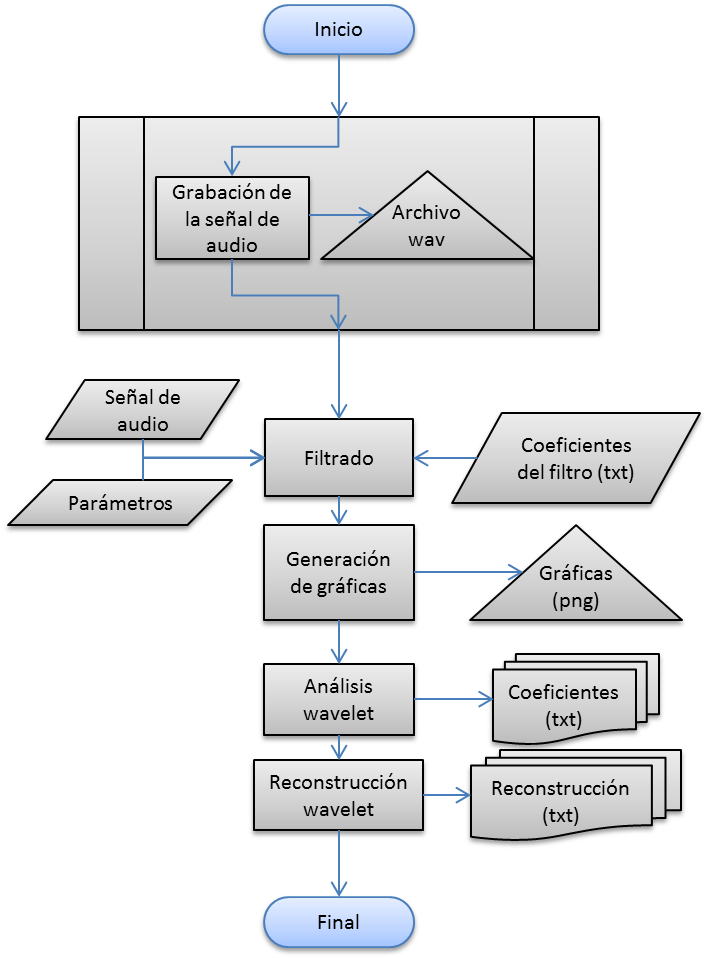
\includegraphics[width=.6\textwidth]{images/diagrama-flujo.png}
	\caption{Diagrama de flujo del algoritmo desarrollado en Python}
	\label{F-diagrama-flujo}
\end{figure}

%PENDIENTE: Se puede modificar para que explique las clases que cree y use:
%Hablar de las clases que use, definirlas y explicarlas.\\
%Diagrama de flujo del algoritmo.\\
%Diagrama de flujo de la GUI.


%------------------------ Implementación -----------------------------%
%Que hice en mi trabajo
% arme el dispositivo
% configuracion, rasbian, backups, wifi
% overclock
% se trabajo con adc click
% hice la herramienta de analysis.py
% - grabar wav
% - fft
% - filtros
% - realizar graficas
%http://docs.scipy.org/doc/scipy/reference/generated/scipy.signal.periodogram.html#scipy.signal.periodogram
% - lectura y escritura de archivos de texto
% - analisis wavelet (wavedec, dwt)
% - reconstruccion analisis wavelet
% hice la gui
% - todo lo que lleva
% arranque en openbox, gui con terminal

%-------------------------- Resultados -------------------------------%
%Que obtuve en mi trabajo
\cleardoublepage
\section{Resultados}
\label{S-resultado}
%-------------- Coeficientes y validación (Resultados) ---------------%
%%\subsection{Coeficientes y validación}
%Resultado: hice un buen análisis Wavelet?
%validación con matlab
%validación con bibliografía
Los resultados del análisis wavelet desarrollado fueron comparados con el \textit{Wavelet Toolbox} de Matlab\textregistered, en el proceso se tomaron en cuenta los primeros 8 decimales de cada coeficiente y cada reconstrucción calculada, el resultado fue de uno a uno. Matlab\textregistered también fue utilizado para validar la implementación de los filtros, aplicándolos a grabaciones previamente realizadas.\\

Por otra parte, en el anteproyecto se propuso como resultado de la elaboración de este trabajo, un prototipo para el desarrollo de pruebas piloto del proyecto de investigación mencionado en el planteamiento del problema, ``\emph{Reconocimiento de emociones}'', y que cumpliese con los requerimientos de la etapa de diseño conceptual. En esta sección se expone el dispositivo resultado de este trabajo, en el formato de un \textit{datasheet}.

%--------------------- Datasheet (Resultados) ------------------------%
%A continuación se expone el dispositivo resultado de este trabajo, en un formato basado en un \textit{datasheet}.
%\subsection{Dispositivo}
\label{S-datasheet}
%-Features
\subsection{Características}
\begin{itemize}[nolistsep]
	\item Adquisición y digitalización de audio
	\item Múltiples frecuencias de muestreo (Fs)
	\item Múltiples tiempos de adquisición de la señal
	\item Almacenamiento temporal de la señal de audio
	\item Aplicación de filtros según los coeficientes suministrados por el usuario en una un archivo de texto plano
	\item Gráfica del espectro temporal de la señal
	\item Gráfica del espectro en frecuencia de la señal
	\item Análisis de la señal adquirida por medio de la transformada wavelet
	\item 76 opciones de wavelets para el análisis % Matlab tiene: 76 + 25db + 25sym
	\item Múltiples niveles de descomposición (El máximo nivel depende de la Fs, el tiempo y la familia utilizada)
	\item Múltiples modos de extensión para la transformada wavelet %http://www.mathworks.com/help/wavelet/ref/dwtmode.html
	\item Entrega de los coeficientes de aproximación y detalle de cada nivel en un archivo de texto plano
	\item Entrega de la reconstrucción de la señal a partir de cada coeficiente entregado
%	\item Análisis de señales de audio grabadas externamente [wav] % Sólo wav?
%	\item Sistema de inferencia básico de emociones
	\item Interfaz gráfica de usuario
	\item Ventana de configuración
	\item Cálculo autónomo del máximo nivel de descomposición
	\item Ventana de información general
	\item Visualización de los coeficientes del filtro desde la interfaz
	\item Visualización de los coeficientes calculados desde la interfaz
	\item Visualización de las reconstrucciones calculadas desde la interfaz
	\item Función de reinicio del programa
	\item Función de apagado del dispositivo desde la interfaz
	\item Comunicación SSH para la copia de archivos
\end{itemize}

%-Applications
\subsection{Aplicaciones}
\begin{itemize}
	\item Adquisición y digitalización de señales de audio con la posibilidad de realizar un filtrado basado en los coeficientes de la transformada Z del filtro. La versatilidad del dispositivo permite aplicar filtros FIR\nomenclature{FIR}{Respuesta finita al impulso, por sus siglas en inglés} o IIR\nomenclature{IIR}{Respuesta infinita al impulso, por sus siglas en inglés}.
	\item Análisis wavelet multiresolución con 76 tipos de wavelets distribuidos en 7 familias, con 6 modos diferentes de extensión para la DWT.
	\item Plataforma para un sistema de inferencia de reconocimiento de emociones basado en el análisis multiresolución de señales de audio.
%	\item Análisis wavelet multiresolución de señales de audio previamente adquiridas.
\end{itemize}
% enfocado al reconocimiento de señales
%Sensor Interface
%Process Control
%Data Acquisition
%Battery Operated Systems

%-Description (overview)
\subsection{Descripción}
El objetivo de este prototipo es realizar análisis de señales por medio de la DWT y está orientado a que sus resultados sean empleados en el reconocimiento de emociones, aunque es importante resaltar que también pueden ser empleados en otras áreas donde el usuario lo desee. Este dispositivo cuenta con la capacidad de adquirir señales de audio de diferentes duraciones y con múltiples Fs\nomenclature{Fs}{Frecuencia de muestreo}, almacenando temporalmente el registro en un archivo de formato wav (\textit{Waveform Audio File Format}), además, genera el espectro temporal (Amplitud vs Tiempo(ms)) y el espectro en potencia (Potencia(dB) vs Frecuencia(Hz)) de la señal. Adicionalmente, tiene la opción de aplicar un filtro FIR o IIR a la señal adquirida. \\

Por otra parte, el dispositivo es capaz de realizar análisis multiresolución con la DWT de la señal adquirida con 6 diferentes modos de extensión y 76 opciones de wavelets, entre las que se encuentran 20 de la familia Daubechies. Debido a que el nivel máximo del análisis multiresolución depende de Fs, el tiempo y la familia utilizada, el dispositivo asiste al usuario al auto-calcular su valor. Como resultado del análisis se generan 2 archivos de texto plano (txt) con los coeficientes de aproximación y detalle de cada nivel y la reconstrucción de la señal a partir de cada coeficiente entregado, de modo que el usuario pueda conocer los componentes de la señal pertenecientes a cada nivel. \\

Para facilitar la interacción con el usuario, el dispositivo cuenta con una GUI\nomenclature{GUI}{Interfaz gráfica de usuario, por sus siglas en inglés}, la cual posee menús de configuración, información general y visualización de archivos planos, así como también funciones de reinicio del programa y apagado del dispositivo. Además, el dispositivo tiene la opción de responder a conexión SSH\nomenclature{SSH}{Secure Shell} para la copia de archivos desde y hacia él. \\

Este dispositivo está inspirado en la autonomía e independencia de los periféricos, por lo cual cuenta con puertos que siguen estándares universales, así garantizar que los elementos conectados al dispositivo pueden ser reemplazados dependiendo de las circunstancias del usuario o deterioro de los mismos, conservando los parámetros expuestos en esta guía (\seccion{S-datasheet}).

%Interfaz gráfica de usuario (GUI)
%Secure Shell (SSH)
%Quien es...\\
%Que hace...\\
%Como lo hace...\\
%Para que lo hace...

%-Diagram (functional block diagram)
\subsection{Diagrama funcional}
El diagrama funcional del dispositivo en la configuración estándar se muestra en la \figura{F-diagrama-func} y en la configuración necesaria para la conexión SSH en la \figura{F-diagrama-func-hub}. Los cuadros grises indican el dispositivo y sus elementos internos, los cuadros azules indican los puertos y los cuadros verdes indican los elementos externos; a su vez las flechas azules indican las conexiones externas y las negras indican las internas.
\begin{figure}[h!]
	\centering
	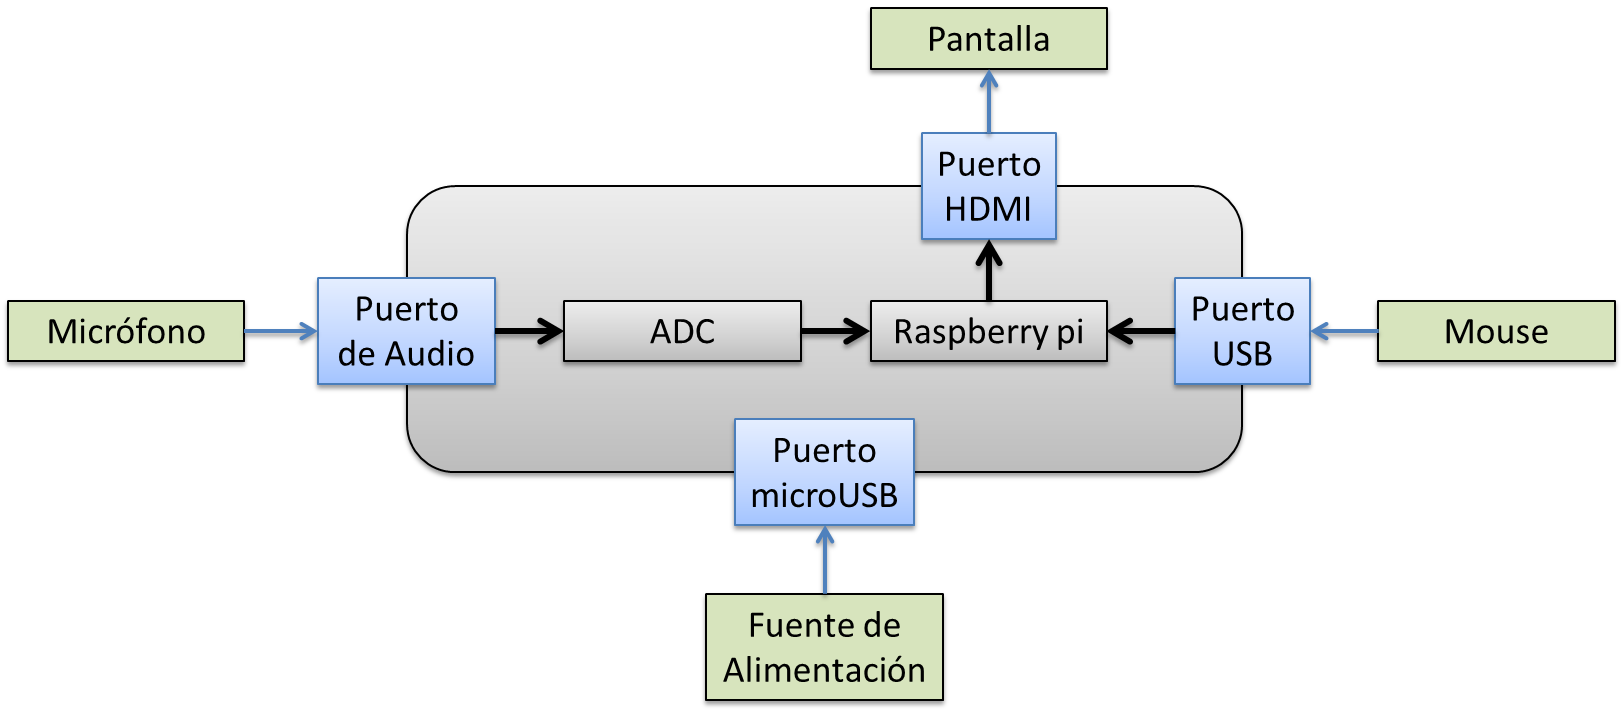
\includegraphics[width=.9\textwidth]{images/diagrama-funcional.png}
	\caption{Diagrama funcional del dispositivo, configuración estándar}
	\label{F-diagrama-func}
\end{figure}

\begin{figure}[h!]
	\centering
	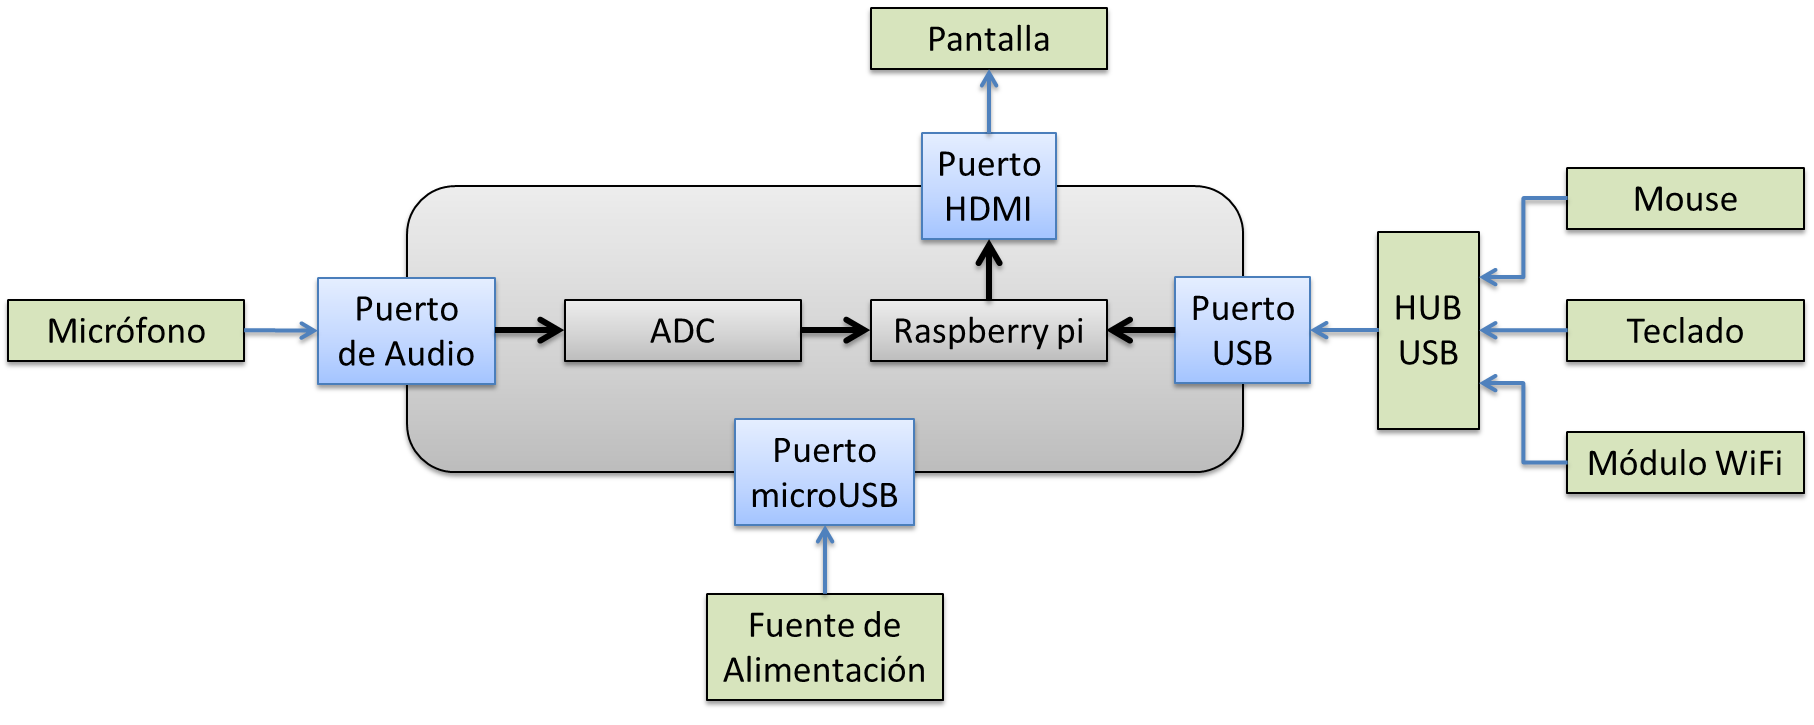
\includegraphics[width=.9\textwidth]{images/diagrama-funcional-hub.png}
	\caption{Diagrama funcional del dispositivo, configuración necesaria para SSH}
	\label{F-diagrama-func-hub}
\end{figure}

%-1.0 Electrical characteristics
\subsection{Características eléctricas}
\label{S-carac-elec}
La alimentación de corriente eléctrica del prototipo se realiza a través de una conexión microUSB y tiene un consumo de potencia de 7W\nomenclature{W}{Vatios} con los periféricos empleados en la configuración estándar (expuesta en la \seccion{S-datasheet}), este valor puede variar en caso de que el usuario reemplace alguno de los elementos. La fuente estándar tiene una entrada AC de 100-240V a 50/60Hz, proporciona una salida USB (5V DC) a un máximo de 2A y se conecta al dispositivo por medio de un cable USB-microUSB (\seccion{S-fuente}). En un caso particular, el usuario podrá reemplazar fácilmente la fuente de potencia debido a que la mayoría de los equipos celulares de nueva generación e incluso agendas electrónicas y \textit{tablets} utilizan el mismo tipo de conexión, esto no es recomendable, pero de realizarlo es necesario tener en cuenta que la nueva fuente deberá ser de buena calidad y estar en la capacidad de suministrar la potencia requerida.
%Conexiones consumo (tomar de un manual de usuario de impresora...)

%-3.0 Pin descriptions
\subsection{Descripción de los puertos}
El dispositivo cuenta con 4 puertos. La alimentación, expuesta en la \seccion{S-carac-elec}, y 3 puertos para periféricos. Cuenta con una salida HDMI en la que se pueden conectar diversos tipos de dispositivos de visualización (monitores y televisores de diferentes especificaciones), la interfaz gráfica está diseñada para un monitor de 32', por lo cual es posible que la distribución se altere si cambian las dimensiones. \\

Los puertos restantes son entradas, uno de ellos es un \textit{jack} estándar de audio para un micrófono, esto garantiza que de ser necesario el usuario tendrá la posibilidad de cambiar el micrófono, el nuevo deberá estar diseñado o tener un comportamiento adecuado para el rango de frecuencias que cubre la voz humana promedio, con el fin de obtener resultados adecuados. El último es un puerto USB, éste está diseñado para la conexión de un \textit{mouse} y con él controlar la GUI, adicionalmente se puede emplear un hub USB para conectar un módulo WiFi y realizar una copia de archivos por medio de una conexión SSH desde un computador.

%Que hace cada uno\\
%Elementos externos:\\
%Mouse\\
%Micrófono\\
%Monitor HDMI\\

\subsection{Componentes}
Para la interacción con el usuario el dispositivo hace uso de elementos externos. Para la entrada de información utiliza un \textit{mouse} por medio del puerto USB y para la salida, una pantalla por medio del puerto HDMI. Mientras que para la adquisición, digitalización y procesamiento de la voz los elementos son externos e internos: un micrófono, una tarjeta de sonido que funciona como ADC y el núcleo de procesamiento, un Rpi. Estos elementos se explican más profundamente a continuación:

\begin{enumerate}
	\item Pantalla: Elemento externo de conexión HDMI. Es un periférico de salida para la comunicación dispositivo-usuario.
	\item \textit{Mouse}: Elementos externo de conexión USB. Es un periférico de entrada con el cual el usuario puede controlar el dispositivo desde la GUI.
	\item Micrófono: Elemento externo, la conexión se realiza por medio de un plug de audio. Es un periférico de entrada con el cual se adquiere la señal de la voz humana a analizar. El dispositivo cuenta con un micrófono Genius MIC-01A, sus características se muestran en la \tabla{T-mic}.
	\item Tarjeta de sonido: Elemento interno de conexión USB. Este cumple la función de un convertidor analógico-digital, el cual recibe la señal eléctrica analógica enviada por el micrófono y la convierte en una señal digital para que el procesador la pueda manipular. El dispositivo posee una tarjeta de sonido Dynamode 3D SOUND (USB-SOUNDCARD2.0), sus características se observan en la \tabla{T-audio-usb}.
	\item Raspberry Pi\textregistered\ (Rpi): Elemento interno. Es el núcleo de el dispositivo, es el encargado de concentrar los periféricos, realizar los cálculos y generar la GUI. Sus características se visualizan en la \tabla{T-rpi}.
\end{enumerate}

%-4.0 Device operation (Convertion) (interno)
\subsection{Operación interna}
\label{S-operacion}
El funcionamiento general se divide en 4 etapas: adquisición y digitalización, pre-procesamiento, procesamiento y generación de resultados. En la etapa de adquisición y digitalización, la señal de audio ingresa al dispositivo a través del micrófono, donde se convierte la energía sonora en energía eléctrica, internamente se utiliza una tarjeta de sonido como ADC y por último el Rpi almacena temporalmente la información en un archivo de audio de formato wav. Tanto esta fase como las siguientes dependen de los parámetros que se utilicen, estos son:
\begin{enumerate}
	\item Frecuencia: Representa la frecuencia de muestreo en Hz con la que se adquirirá la señal, para evitar tiempos elevados de procesamiento se recomienda utilizar una baja. Predeterminada: 8kHz. Totales disponibles en el dispositivo:
	\begin{multicols}{2}
		\begin{itemize}[nolistsep]
			\item 8000
			\item 11025
			\item 16000
			\item 22050
			\item 32000
			\item 44100
			\item 48000
		\end{itemize}
	\end{multicols}

	\item Tiempo: Representa el tiempo de adquisición de la señal, en segundos. Predeterminada: 3s. Totales disponibles en el dispositivo:
	\begin{multicols}{2}
		\begin{itemize}[nolistsep]
			\item 2
			\item 2.5
			\item 3
			\item 3.5
			\item 4
			\item 4.5
		\end{itemize}
	\end{multicols}
\end{enumerate}

Las etapas descritas a continuación son realizadas en el núcleo de procesamiento a través del lenguaje de programación Python. Los archivos pertinentes se encuentran almacenados en el directorio \textit{``/home/pi/proyecto\_pi''}, el cual se denominará directorio raíz. El archivo de audio es almacenado temporalmente en la carpeta \textit{``audio''} en el directorio raíz, con el nombre \textit{``audio.wav''} \\

En el pre-procesamiento de la señal existe la opción de aplicar un filtro, esto se realiza a partir de los coeficientes de la transformada Z hallados al modelarlo como una planta y calcular su función de transferencia, los cuales deberán estar en archivos de texto plano (txt), uno para el numerador (zeros de la función), llamado \textit{``filter\_zs.txt''} y otro para el denominador (polos de la función), llamado \textit{``filter\_ps.txt''}; estos archivos deberán estar ubicados en una carpeta llamada \textit{``filter''} dentro del directorio raíz. Para que el dispositivo realice el filtrado, el usuario deberá proporcionarle los coeficientes del filtro deseado, separados por una \mbox{coma (,)} o un \mbox{espacio ( )}; por medio de un computador y una conexión SSH, para esto es necesario copiar el archivo con los coeficientes como se indica en la \seccion{S-ssh}. También está habilitada la opción de conectar un teclado por medio de un hub USB y escribir o modificar los coeficientes. No hay ningún filtro predeterminado, en caso de desear utilizar uno, el usuario deberá ir la ventana de configuración de la GUI y cambiar el tipo de filtro a aplicar. Luego del filtrado se generan las gráficas del espectro temporal normalizado y el espectro en frecuencia (en decibeles) de la señal de audio. Las imágenes son almacenadas temporalmente en formato png (\textit{Portable Network Graphics}) en la carpeta \textit{``images''} en el directorio raíz, con los nombres de \textit{``tspectrum.png''} para el espectro temporal y \textit{``pspectrum.png''} para el espectro en frecuencia. \\

El procesamiento comprende el análisis wavelet; durante esta etapa se calcula la DWT de la señal de audio con unos parámetros específicos, estos pueden ser cambiados desde la ventana de configuración de la GUI. Adicionalmente en esta etapa se realiza la reconstrucción de la señal original a partir de cada coeficiente arrojado por la descomposición. Los parámetros son:
\begin{enumerate}
	\item Familia: Representa la familia de wavelets a emplear. Predeterminada: \textit{Daubechies} (``db''). Totales disponibles en el dispositivo:
	\begin{itemize}[nolistsep]
		\item \textit{Haar} (``haar'')
		\item \textit{Daubechies} (``db'')
		\item \textit{Symlets} (``sym'')
		\item \textit{Coiflets} (``coif'')
		\item \textit{Biorthogonal} (``bior'')
		\item \textit{Reverse Biorthogonal} (``rbio'')
		\item \textit{Discrete Meyer} (``dmey'')
	\end{itemize}

	\item Wavelet: Representa el tipo de wavelet a emplear, es importante resaltar que por definición ``haar'' y ``db1'' son iguales. Predeterminada: ``db8''. Totales disponibles en el dispositivo:
	\begin{itemize}
		\item \textit{Haar} (``haar'')
		\item \textit{Daubechies} (``db1'', ``db2'', ... ,``db10'', ... , ``db20'')
		\item \textit{Symlets} (``sym2'', ... , ``sym10'', ... ,``sym20'')
		\item \textit{Coiflets} (``coif1'', ... , ``coif5'')
		\item \textit{Biorthogonal} (``bior1.1'', ``bior1.3'', ``bior1.5'', ``bior2.2'', ``bior2.4'', ``bior2.6'', ``bior2.8'', ``bior3.1'', ``bior3.3'', ``bior3.5'', ``bior3.7'', ``bior3.9'', ``bior4.4'', ``bior5.5'', ``bior6.8'')
		\item \textit{Reverse Biorthogonal} (``rbio1.1'', ``rbio1.3'', ``rbio1.5'', ``rbio2.2'', ``rbio2.4'', ``rbio2.6'', ``rbio2.8'', ``rbio3.1'', ``rbio3.3'', ``rbio3.5'', ``rbio3.7'', ``rbio3.9'', ``rbio4.4'', ``rbio5.5'', ``rbio6.8'')
		\item \textit{Discrete Meyer} (``dmey'')
	\end{itemize}

	\item Nivel de profundidad: Representa el máximo nivel del análisis multiresolución. Predeterminado: 3. El total disponible en el dispositivo es calculado y mostrado en la ventana de configuración, pues varía con los demás parámetros seleccionados (Tiempo, frecuencia de muestreo, familia y wavelet) por lo cual no es posible enumerar cada caso en este documento. Por ejemplo, con un tiempo de 3s, una frecuencia de muestreo de 8kHz, una familia \textit{Daubechies} y un tipo de wavelet ``db8'', el máximo nivel de descomposición es 10, lo que nos permite un análisis multiresolución máximo de 10 niveles.

	\item Modo: Representa el modo de extensión a emplear, se utiliza para extender el vector original de la señal y realizar el análisis wavelet sobre un vector del tamaño de una potencia de 2. Predeterminado: \textit{Symmetric padding} (``sym''). Totales disponibles en el dispositivo:
	\begin{multicols}{2}
		\begin{itemize}
			\item \textit{Zero padding} (``zpd'')
			\item \textit{Constant padding} (``cpd'')
			\item \textit{Symmetric padding} (``sym'')
			\item \textit{Periodic padding} (``ppd'')
			\item \textit{Smooth padding} (``sp1'')
			\item \textit{Periodization} (``per'')
		\end{itemize}
	\end{multicols}
\end{enumerate}

En la etapa final llamada generación de resultados, se almacenan los resultados de la fase anterior en un txt de manera que el usuario pueda visualizarlos ya sea a través de los menús \textit{Show Coefficients}, \textit{Show Audio Reconstruction} o de la copia del archivo por medio de otro computador y una conexión SSH. Los archivos son almacenados temporalmente en la carpeta \textit{``coef''} en el directorio raíz, con los nombres de \textit{``coef\_dwt\_''} para los coeficientes y \textit{``audio\_reconstruction\_dwt\_''} para las reconstrucciones de la señal de audio, seguidos del tipo de wavelet y el nivel utilizado; por ejemplo con un tipo de wavelet ``db8'' y un nivel de descomposición de 2, los nombres de los archivos serán \textit{``coef\_dwt\_db8\_2.txt''} y \textit{``audio\_reconstruction\_dwt\_db8\_2.txt''}. \\

Los archivos de salida son reemplazados con cada ejecución del programa y no son borrados cuando el dispositivo se apaga.\\

La \tabla{T-complejidad} muestra de manera general la complejidad algorítmica de los algoritmos utilizados y la complejidad resultante, $N$ representa el número de datos entrantes (del orden de $10^4$) y $m$ el nivel del análisis multiresolución (del orden de $20$). De este modo, se puede decir que la complejidad algorítmica del software del dispositivo es logarítmica lineal \cite{Arora2009}. \label{S-complejidad}
\begin{table}[H]
	\begin{center}
		%\resizebox{\textwidth}{!}{
		\begin{tabular}{|c|c|}
			\hline
			Algoritmo & Complejidad \\ \hline
			FFT\nomenclature{FFT}{Transformada rápida de Fourier, por sus siglas en inglés} & $O(N\log(N))$\cite{Rioul1992} \\ \hline
			DWT & $O(N)$\cite{Rioul1992} \\ \hline
			iDWT\nomenclature{iDWT}{Transformada wavelet discreta inversa, por sus siglas en inglés} & $O(N)$\cite{Rioul1992} \\ \hline
			Total & $O(N\log(N)) + mO(N) + mO(N)$ \\ \hline
		\end{tabular}
		%}
	\end{center}
	\caption{Complejidad algorítmica del software del dispositivo}
	\label{T-complejidad}
%http://www.geniusnet.com/wSite/ct?xItem=16664&ctNode=145
\end{table}

%Que usa y como hace su tarea\\
%USB -> Mouse\\
%Audio USB -> Micrófono\\
%Salida -> Monitor HDMI\\

\subsection{Utilización}
\label{S-utilizacion}
%finalmente al pulsar el botón de \textit{Start}
El usuario deberá conectar los periféricos (El \textit{mouse}, la pantalla y el micrófono) antes de conectar el dispositivo a la corriente eléctrica (cable michoUSB), se encenderá el prototipo y comenzará a cargar los paquetes necesarios para el funcionamiento. Al finalizar, aparecerá un pantalla negra y el puntero del \textit{mouse}, a este punto se denominará pantalla de inicio. \\

%%-5.0 Serial communication (salida del dispositivo)
\textbf{Interfaz gráfica de usuario.}
%Visualización de los resultados, gráficas y archivos de texto\\
%visualización del filtro\\
%-> Consumió mucho tiempo!!! mostrar mostrar mostrar screenshots!\\
% Modos de operacion (tiempo real)
Al hacer \textit{click} derecho aparecerá un menú de opciones, para abrir la GUI seleccione \textit{``Terminal emulator''}, al hacer esto aparecerá una terminal tipo linux y luego la GUI, la cual muestra una bienvenida y la pantalla principal (\figura{F-gui-principal}). Allí, el usuario tiene acceso a los botones y menús.
\begin{enumerate}
	\item Botón \textit{``Start''}: Comienza la captura de la voz, el primer análisis y la presentación de las gráficas del audio, la tercera imagen representa el lugar reservado para la emoción reconocida por medio de un sistema de inferencia propuesto para un trabajo futuro (\seccion{S-trabajofuturo}). Este botón es rojo cuando el \textit{mouse} pasa sobre él y durante el periodo de adquisición de la señal, lo cual sirve como indicador visual para el usuario, se recomienda que el puntero del \textit{mouse} se aleje del botón luego de haberlo pulsado, para que el indicador visual pueda ser efectivo.
	\item Botón \textit{``Wavelet analysis''}: Este botón ejecuta el análisis wavelet sobre la grabación realizada con el botón \textit{``Start''} con los parámetros especificados en la ventana de configuración, por lo cual, si el usuario desea realizar análisis con diferentes parámetros sobre la misma grabación, sólo deberá ir a la ventana de configuración seleccionar los parámetros deseados y pulsar este botón.
	\item Botón \textit{``Stop''}: Este botón está diseñado para el modo de operación en tiempo real que se propone en el trabajo futuro (\seccion{S-trabajofuturo}), este detendría el proceso continúo de grabación.
	\item Menú \textit{``Menu''}: Contiene los siguientes submenús de la herramienta:
	\begin{itemize}
		\item \textit{``Configuration''}: Abre la ventana de configuración, donde se muestran y realizan cambios a los parámetros para la adquisición y digitalización, el filtrado y el análisis. Cuenta con un botón \textit{``ok''} y uno \textit{``reset''}.
		\item \textit{``Show Filter Zeros''}: Muestra el documento de texto plano con los coeficientes del filtro pertenecientes al numerador, si no se ha encontrado un filtro muestra un cuadro de dialogo informándolo.
		\item \textit{``Show Filter Polos''}: Muestra el documento de texto plano con los coeficientes del filtro pertenecientes al denominador, si no se ha encontrado un filtro muestra un cuadro de dialogo informándolo.
		\item \textit{``Show Coefficients''}: Muestra el documento de texto plano con los coeficientes del último análisis wavelet, si esto no se ha realizado la herramienta lo hace; para esto es necesario haber pulsado el botón \textit{``Start''} para realizar la grabación de la voz, si esto no sea ha hecho muestra un cuadro de dialogo informándolo.
		\item \textit{``Show Audio Reconstruction''}: Muestra el documento de texto plano con las reconstrucciones de los coeficientes del último análisis wavelet, si esto no se ha realizado la herramienta lo hace; para esto es necesario haber pulsado el botón \textit{``Start''} para realizar la grabación de la voz, si esto no sea ha hecho muestra un cuadro de dialogo informándolo.
		\item \textit{``Restart''}: Cierra e inicializa nuevamente la GUI.
		\item \textit{``Turn off''}: Muestra una venta de verificación y apaga el dispositivo.
	\end{itemize}
	\item Menú \textit{``About''}: Muestra una ventana de información general acerca de la herramienta y sus desarrolladores.
\end{enumerate}

\begin{figure}[h!]
	\centering
	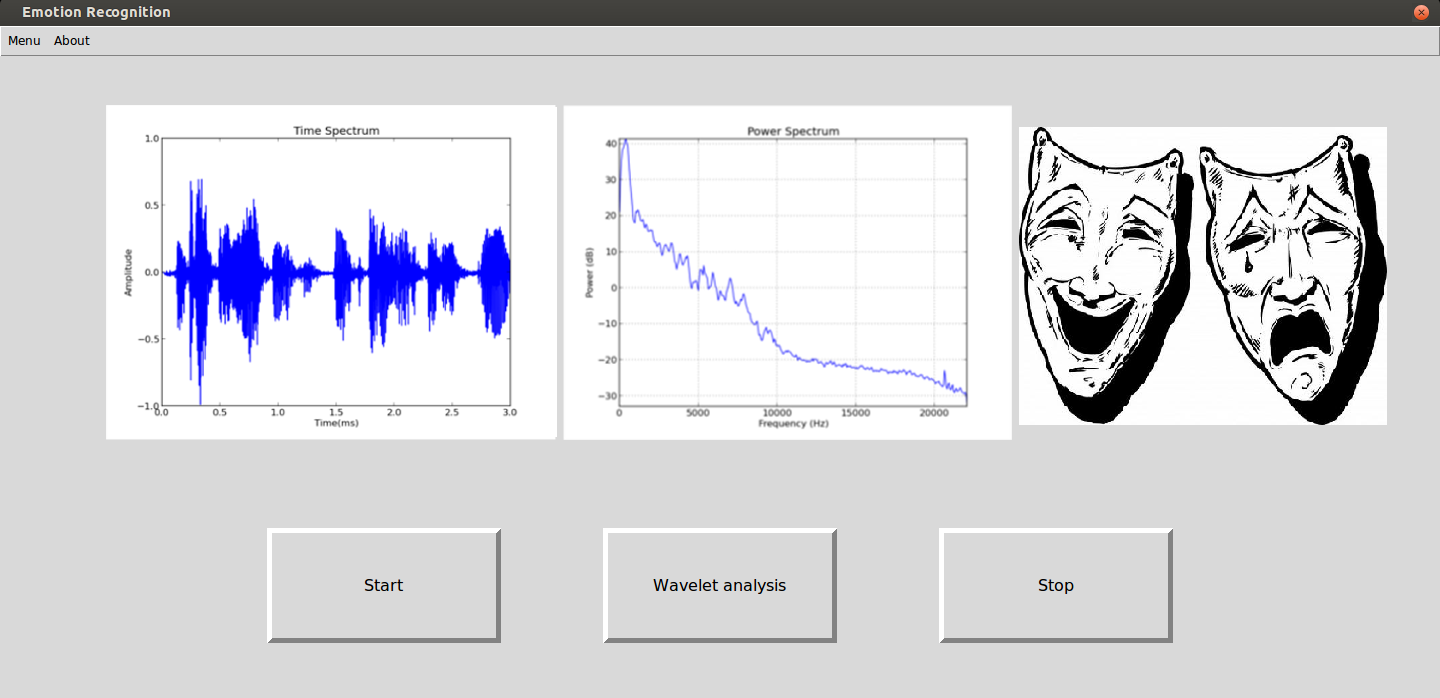
\includegraphics[width=1\textwidth]{images/gui-principal.png}
	\caption{Vista principal de la GUI}
	\label{F-gui-principal}
\end{figure}

\textbf{Configuración de red y conexión SSH.} \label{S-ssh}
Si el usuario desea realizar una conexión SSH con el dispositivo, primero deberá configurar la conexión inalámbrica a través de una ventana de configuración externa a la GUI (el proceso es igual a como se hace en cualquier computador, buscar la red, seleccionarla y escribir su contraseña), para acceder a ella se debe dar \textit{click} derecho en la pantalla de inicio, luego \textit{click} en \textit{Debian}, \textit{Applications}, \textit{Network}, \textit{Monitoring} y puedo \textit{click} en \textit{wpasupplicant user interface}. Para habilitar esta opción el usuario deberá conectar un hub USB al puesto USB del dispositivo y luego un módulo Wifi, un teclado y el \textit{mouse} a dicho hub. Luego de la configuración no se requiere el teclado para conexiones futuras. \\

El dispositivo activa la conexión SSH, se aconseja realizar el intercambio de archivos desde el computador. En esta configuración el dispositivo responde a los comandos estándar de SSH, por ejemplo, desde una terminal linux el comando de copia de archivos sería: \mbox{{\footnotesize scp \textit{archivo\_a\_copiar} pi@\textit{IP\_del\_dispositivo\_dentro\_de\_la\_red}:\textit{directorio\_raiz/directorio\_de\_destino}}}.

%Que usa y como hace su tarea\\
%como correr el algoritmo \\
%analysis.py \\
%gui\_proyecto.py \\
%ssh

%-2.0 Typical performance characteristics
%\subsubsection{Características de desempeño.}
%En la configuración del dispositivo se encuentran los parámetros pertinentes para la adquisición y el análisis wavelet deseado
%Gráficas de respuestas \\
%Frecuencias

%%Formato de salida? SSH?
%\subsubsection{Archivos de salida}
%Salen gráficas[png] y archivos de texto[txt]
%%copia desde USB
%%copia desde red (ssh)

%-6.0 Applications information (Using, Layouts) (a tener en cuenta...)
\subsection{Precauciones y consideraciones}
Durante la manipulación del dispositivo el usuario deberá tener ciertas precauciones, para evitar riesgos, y consideraciones, para evitar problemas de mal funcionamiento. \\
Precauciones:
\begin{itemize}
	\item Tenga precaución con el suministro eléctrico, si no lo hace puede salir herido.
	\item Tenga precaución con los cables, halarlos o desconectarlos bruscamente puede dañar o deteriorar los cables o el dispositivo.
	\item Evite obstruir el ventilador del dispositivo que está ubicado en la parte inferior. Este es necesario para refrigeración, si esto no se realiza adecuadamente el prototipo puede deteriorarse e incluso dañarse.
	\item Se recomienda utilizar la fuente proporcionada con el dispositivo, si esta va a ser reemplazada, tenga en cuenta los parámetros establecidos en la \seccion{S-carac-elec}, otros elementos pueden dañar o disminuir el desempeño del prototipo.
\end{itemize}
Consideraciones:
\begin{itemize}
	\item La GUI fue diseñada para una pantalla de 32', utilizar un tamaño diferente puede alterar la distribución de los iconos, botones e imágenes.
	\item El dispositivo fue diseñado para trabajar con micrófonos genéricos, pero debe tener en cuenta el rango de respuesta en frecuencia del mismo para garantizar que la voz está siendo adquirida adecuadamente.
\end{itemize}

%Consideraciones...\\
%Micrófonos: respuestas en frecuencia, la mayoría vienen diseñados para voz (8k)\\
%Temperatura: precaución, no interfiera el cooler\\
%Monitor HDMI: resolución propuesta() y tamaño (pulgadas) la distribución de la interfaz gráfica se puede alterar\\
%Fuente: Usar los elementos proporcionados, otros elementos pueden dañar o disminuir el desempeño (Potencia)\\

%-7.0 Packaging information (map, CAD, physical)
\subsection{Información  física}
La forma física del dispositivo busca inspirar estabilidad, ser llamativa y amigable con el usuario. Este último punto está unido a la utilización de cables y elementos estándar que el usuario fácilmente conoce de antemano. En la \figura{F-carcasa-anterior} y la \figura{F-carcasa-posterior} se pueden visualizar las vistas anterior y posterior de la carcasa.

\begin{figure}[h!]
	\centering
	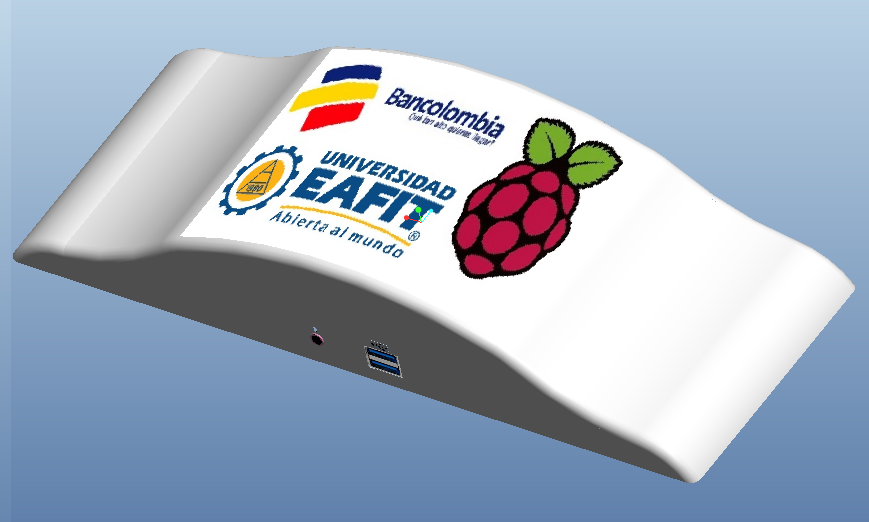
\includegraphics[width=.6\textwidth]{images/carcasa-anterior.png}
	\caption{Vista anterior de la carcasa}
	\label{F-carcasa-anterior}
\end{figure}
\begin{figure}[h!]
	\centering
	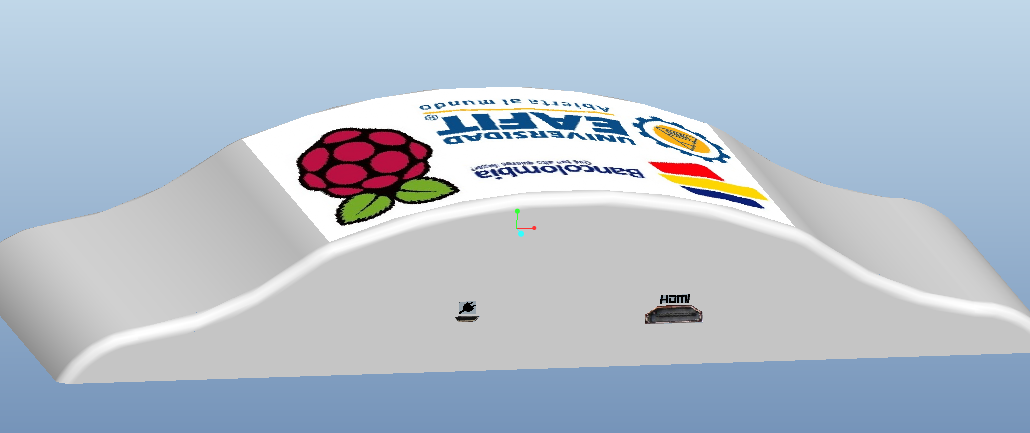
\includegraphics[width=.6\textwidth]{images/carcasa-posterior.png}
	\caption{Vista posterior de la carcasa}
	\label{F-carcasa-posterior}
\end{figure}

%Parte física del dispositivo: forma, dimensiones, planos, materiales, implementos, cables y conxiones

%Appendix
\subsection{Planos}
Los planos del dispositivo se muestran en la \figura{F-planos}.
\cleardoublepage
%\includepdf[pages=-, landscape=true]{images/rpi_plano.pdf} \label{F-planos}
%\begin{figure}[h!]
%	\centering
%	\includegraphics[width=1\textwidth]{images/rpi_plano.pdf}
%	\caption{Planos del dispositivo}
%	\label{F-planos}
%\end{figure}

%------------------- Analisis de resultados --------------------------%
%\section{Análisis de resultados}
%Lucia: Errores y problemas encontrados
%Analizar los cambios en el dispositivo
%todo se basa en el Fenómeno físico
%
%python es bueno?
%el algoritmo es bueno?
%el metodo, wavelet es bueno?
%es posible pensar en reconocer emociones?
%el dispositivo es bueno?

%------------------------- Conclusiones ------------------------------%
\cleardoublepage
\section{Conclusiones y trabajo futuro}
\label{S-conclusiones}
%Es una parte importante de la tesis donde el autor emite juicios con relación a su hipótesis, la refuta o la comprueba basado en una síntesis de los resultados obtenidos. Las conclusiones deben reflejar los alcances y las limitaciones del estudio, las recomendaciones que puedan ser útiles al problema de investigación, así como las consecuencias y determinaciones que puedan contribuir al desarrollo del conocimiento. Algunos de los aspectos que se sugiere incorporar son:
%  Resultados obtenidos.
%  Comprobación / refutación de la hipótesis.
%  Conclusión general
%  Aportación al campo o disciplina.

%Las conclusiones responden a los objetivos con cosas puntuales.
%O sea... usted tenía unos objetivos para cuyo alcance desarrollo unas actividades, obtuvo unos resultados que analiza/discute y finalmente responde a esos objetivos.
%Es decir, la "carreta" va en el análisis/discusión, en las conclusiones se responde de forma puntual a lo que se pretendía hacer/resolver


%Conclusiones
% Adc click muy lento bajo esta aplicacion, maximo de 5k-8k
% Utilidad y futuro de Audio-USB (osciloscopio)
%- Muy buen futuro para el analisis de emociones
%- Wavelet validadas, ende analisis es bueno
%- Cambiar los tiempos para que den cantidades de datos multiplos de 2
%- 
%- 
%- ES BUENO O NO EL RESULTADO?
%
%
% Diseño conceptual del dispositivo, partiendo de la identificación de los requerimientos técnicos y del usuario.
% Diseñar las etapas de adquisición, pre-procesamiento y procesamiento de la señal de audio.
%%\ Diseñar y desarrollar el algoritmo de análisis de la señal.
% Construir la planta física y verificar la correcta comunicación entre los periféricos utilizados.
% Digitalizar la señal de audio por medio del convertidor analógico digital escogido en el diseño conceptual, teniendo en cuenta el análisis espectral de la señal fenomenológica aplicando conceptos básicos de muestreo y retención de datos.
% Desarrollar los algoritmos de pre-procesamiento y procesamiento de la señal.
%%\ Implementar filtros para la señal adquirida.
%Implementar los algoritmos desarrollados.
%Realizar pruebas del dispositivo piloto final para evaluar su desempeño, por medio de la comparación con herramientas de programación ya validadas o datos reportados en la literatura.
\subsection{Conclusiones}
\begin{itemize}
%- Adc click muy lento bajo esta aplicacion, maximo de 5k-8k
	\item  Durante el desarrollo se buscó implementar un ADC click, cuyo chip principal es el MCP3204 y con comunicación SPI, para la digitalización de señales de audio. A pesar de que este tiene una frecuencia nominal de trabajo de 50ksps; al probarlo en el montaje no se alcanzó la frecuencia requerida por el fenómeno físico. Por esto se concluyó que este elemento no es adecuado para aplicaciones de audio, aunque puede ser muy útil en fenómenos de respuesta más lenta, calor por ejemplo.
	
%- Utilidad y futuro de Audio-USB (osciloscopio)
	\item Una tarjeta de sonido es un hardware con muy buenas prestaciones como ADC, diferentes frecuencias de muestreo e incluso algunas son multicanal o permiten variar la resolución; y se encuentran en el mercado diversas calidades y precios. Su fácil conexión con un computador o, en el caso de este proyecto, un Rpi, junto con la variedad de software disponible para acceder a ella, ya sea directa (por medio de un código desarrollado en C++, Matlab\textregistered\ o Python) o indirectamente (por medio del OS u algún otro programa como ALSA); hace que tengan un buen potencial en aplicaciones científicas o ingenieriles de bajo costo, esto ha sido explorado en trabajos como los realizados por Tang \cite{Tang2005} y Azooz \cite{Azooz2006}.

%%- Posible tiempo real por la complejidad algorítmica
	\item Con la complejidad computacional de los algoritmos implementados, expuesta en la \seccion{S-complejidad}, es posible plantear un trabajo futuro sobre la extensión del prototipo a ejecución en tiempo real, entendiendo esto como que el algoritmo sea capaz de correr completamente en el tiempo en el que se realiza una grabación. Aunque tal vez sí sea necesario pensar en algún cambio externo al algoritmo, como considerar un lenguaje copilado, una forma diferente de mostrar las gráficas de salida, un hardware con más capacidad o eliminar la GUI, debido a que esta consume mucho procesamiento.

%% Diseño conceptual del dispositivo, partiendo de la identificación de los requerimientos técnicos y del usuario.
%	\item 

%% Diseñar las etapas de adquisición, pre-procesamiento y procesamiento de la señal de audio.
	\item Se diseñaron las diferentes etapas del dispositivo por medio del estudio de la bibliografía del fenómeno físico y el marco teórico; además se llevaron a cabo experimentos con señales de audio que permitieron validar esos conceptos. Aún así, aunque este estudio mostró que había unas características necesarias, que fueron satisfechas en el proyecto, se quiso dar más libertad al usuario de modo que pudiese variar los parámetros de grabación y análisis, con el fin de que este dispositivo pueda ser utilizado para la identificación de patrones en la voz que contengan información sobre las emociones de un interlocutor, para finalmente diseñar un sistema de inferencia que permita reconocer emociones a partir de una señal de audio.

%%%\ Diseñar y desarrollar el algoritmo de análisis de la señal.
%% Construir la planta física y verificar la correcta comunicación entre los periféricos utilizados.
%	\item 

%% Digitalizar la señal de audio por medio del convertidor analógico digital escogido en el diseño conceptual, teniendo en cuenta el análisis espectral de la señal fenomenológica aplicando conceptos básicos de muestreo y retención de datos.
%	\item 

%% Desarrollar los algoritmos de pre-procesamiento y procesamiento de la señal.
%	\item 

%%%\ Implementar filtros para la señal adquirida.
	\item A pesar de que el filtrado no era un objetivo inicial en el proyecto, se logró que el prototipo final estuviese en la capacidad de aplicar correctamente filtros FIR e IIR a partir de los coeficientes de la transformada Z; esto fue validado por medio de la comparación con resultados obtenidos en Matlab\textregistered.

%%Implementar los algoritmos desarrollados.
%	\item 

%%Realizar pruebas del dispositivo piloto final para evaluar su desempeño, por medio de la comparación con herramientas de programación ya validadas o datos reportados en la literatura.
	\item Las pruebas realizadas sobre el dispositivo y su validación con el \textit{Wavelet Toolbox} de Matlab\textregistered, sugieren que el prototipo desarrollado arroja resultados altamente confiables y reproducibles; no se realizó una validación con la literatura por la dificultad de encontrar los datos necesarios para dicha tarea.

%%- Muy buen futuro para el analisis de emociones
%	\item 

%%- Wavelet validadas, ende analisis es bueno
%	\item 


%"Se comprobó que los resultados arrojados por el diseño conceptual, teniendo en cuenta los requerimientos técnicos y de usuario, permitieron elegir una ruta óptima de construcción del dispositivo piloto, que facilitó y agilizó la labor de ejecución, de lo contrario se habría hecho necesario experimentar con diferentes rutas y elementos, lo cual hubiese tomado más del tiempo estipulado."
\end{itemize}

\subsection{Trabajo futuro}
\label{S-trabajofuturo}
% Trabajo futuro
%- Reconocimiento de emociones
%- Modo de tiempo real:
%   - Un core mas veloz (Rpi)
%   - Interfaz grafica independiente
%   - Aplicacion sin graficas
%   - Lenguaje más rápido (copilado) [c++ tiene librerias WT]

Bajo los resultados alcanzados con este proyecto y el marco general del reconocimiento de emociones, puede ser de interés:

\begin{itemize}
	\item Modificar los tiempos de grabación del dispositivo buscando que se aproximen mejor a una potencia de 2, con el fin de reducir al máximo el \textit{padding} en la transformada wavelet.
	\item Extender el dispositivo para que realice cualquier transformada wavelet a partir de los coeficientes de los filtros pasa bajos y pasa altos.
	\item Estudiar registros acústicos locales de diferentes emociones por medio del análisis wavelet, con el fin de encontrar patrones que sirvan como parámetros de entrada de un sistema de inferencia, podría ser interesante verificar la influencia de elementos variables en los registros como las edades de las personas, el sexo o incluso el idioma. También sería interesante analizar emociones diferentes a las básicas \cite{Pell2011}, entra más emociones se analice más se podrá perfeccionar el sistema de inferencia.
	\item Extender el alcance del proyecto a la identificación precisa de diferentes emociones, por medio de un sistema de inferencia robusto.
%%- Cambiar los tiempos para que den cantidades de datos multiplos de 2
	\item Extender la herramienta a ejecución en tiempo real, para ello es necesario agregar una función que dé continuidad al análisis alcanzado en este trabajo. Con el fin de reducir el tiempo de ejecución puede ser útil considerar un lenguaje de programación compilado, un dispositivo con un procesador más potente o disminuir la carga puesta por agentes externos a este último.
	\item Explorar otros mecanismos de visualización de resultados con el fin de aumentar la portabilidad del dispositivo. También puede ser interesante considerar la utilización de baterías recargables en lugar del cable de poder.
\end{itemize}

%Estudiar de manera más precisa y exaustiva los niveles de desconposicion de los audios para identificar emociones, buscar si hay diferencias enlos idiomas, las edades de las personas, lo sexos.

%estudiar
%explorar
%extender
%contrastar

%lo que hace que el proceso se pueda realizar independiente al programa desarrollado en Python, y así, este último puede correr independiente a la grabación, lo que podría facilitar la implementación en tiempo real propuesta en la sección de trabajo futuro (\seccion{S-trabajofuturo})
%
%Comienza la captura de la voz, el primer análisis y la presentación de las gráficas del audio, la tercera imagen representa el lugar reservado para la emoción reconocida por medio de un sistema de inferencia propuesto para un trabajo futuro (\seccion{S-trabajofuturo}).

%--------------------------- Apendices -------------------------------%
%\newpage
\appendix
\cleardoublepage 
\section{Planos esquemáticos del Rpi}
En las siguientes páginas se adjuntan los planos esquemáticos del Rpi, con el fin de mostrar su contenido electrónico.
%Incluir planos del Rpi (pdf), puede ser como imágenes o agregando las hojas al pdf.
%\includepdf[pages=-, landscape=true]{images/Raspberry-Pi-R2-Schematics.pdf}






%%------------------------ Anteproyecto -------------------------------%
%\cleardoublepage 
%%\newpage
%\mbox{}
%\thispagestyle{empty}
%\newpage
%\chapter{Anteproyecto}
%\newpage

%---------------------- Aspectos legales -----------------------------%
\cleardoublepage \phantomsection
\section*{Aspectos legales}
\addcontentsline{toc}{section}{\protect\numberline{}Aspectos legales}

%%http://www.python.org/psf/trademarks/
``Python'' y los logos de Python son \textit{trademark} de la \textit{Python Software Foundation}, usados por William Sánchez con permiso de la Fundación. \\
%%"Python" and the Python logos are trademarks or registered trademarks of the Python Software Foundation, used by ___________ with permission from the Foundation.


%%http://www.raspberrypi.org/trademark-rules
``Raspberry Pi'' y los logos de Raspberry Pi son \textit{trademark} de la \textit{Raspberry Pi Foundation}, usados por William Sánchez con permiso de la Fundación. \\


%%MATLAB is a registered trademark of The MathWorks, Inc. 
Matlab es un \textit{trademark} de The MathWorks, Inc.




%------------------------- Referencias -------------------------------%
%%%Referencias sin cita en el texto
%%\nocite{}
%\nocite{AnalogDevices2005}
%
%%%Referencias no usadas
%\nocite{Liberman2000a}
%\nocite{WikiEmotion}





\cleardoublepage \phantomsection
\addcontentsline{toc}{section}{\protect\numberline{}\refname}
%\selectbiblanguage{spanish}
%%\bibliographystyle{plain}      % Alfabetico, corchetes
%%\bibliographystyle{ieeetr}     % Orden, corchetes
%%\bibliographystyle{unsrt}      % Orden, corchetes
%%%\bibliographystyle{alpha}      % Alfabetico, abreviaturas
%\bibliographystyle{abbrv}      % Alfabetico, corchetes

%%Para referenciar sin cita en el texto
%\nocite{}
%\cleardoublepage \phantomsection
%\addcontentsline{toc}{chapter}{Referencias}
%\bibliographystyle{babplain}
\bibliographystyle{babunsrt}
%\bibliographystyle{bababbrv}
\bibliography{refapg}

%UNIVERSIDAD EAFIT. BIBLIOTECA LUIS ECHAVARRÍA VILLEGAS. Usando la biblioteca [Online] : página Web.
%Medellín: La Biblioteca, 2005. (Citada: 6 Dic. 2005) http://www.eafit.edu.co/biblioteca/servicios/usandoBiblioteca/index.htm

%Genius. MIC-01A Multimedia Microphone [Online] : página web. Octubre 27, 2009 (Citada: 25 Oct. 2013) http://www.geniusnet.com/wSite/ct?xItem=16664&ctNode=145

%Elinux. RPi Hardware [Online]: página web. Octubre 2013 (Citada: 25 Oct. 2013) http://elinux.org/RPi_Hardware

\end{document} 


%
%%------------------------- Presupuesto -------------------------------%
%\section{Aspectos administrativos}
%\subsection{Presupuesto}
%En la tabla \ref{presupuesto} (al final del documento) se muestra el presupuesto planeado para la ejecución de la propuesta. Es sólo un estimado, así que los elementos y precios pueden variar dependiendo de los resultados que arroje el diseño conceptual. Los precios del hardware presentado no incluyen IVA, mientras que el total sí lo tiene calculado. Para el trabajo con el Raspberry Pi\textregistered \ se requiere un monitor con entrada HDMI, en el caso de que la estación de trabajo no lo posea, habría que comprarlo, por lo cual también se incluye en el presupuesto. Se debe tener en cuenta que no es factible conocer a priori todos los detalles y elementos requeridos, por lo cual es posible que sea necesario comprar algún elemento adicional durante el desarrollo del proyecto.
%
%\begin{table}[!h]
%\begin{center}
%%\resizebox{\textwidth}{!}{
%\begin{tabular}{|c|c|c|c|c|}
%\hline
%Tipo & Item & Valor(COP) & Proveedor & Observación \\ \hline
%
%\multirow{25}{*}{Hardware} & Raspberry Pi\textregistered & 125.000 & \href{http://www.didacticaselectronicas.com/index.php?page=shop.product_details&flypage=flypage.tpl&product_id=1334&category_id=42&keyword=raspberry+pi&option=com_virtuemart&Itemid=134}{Proveedor Universidad} & Procesamiento \\ \cline{2-5}
%
%& Caja Raspberry Pi\textregistered & 22.000 & \href{http://www.didacticaselectronicas.com/index.php?page=shop.product_details&flypage=flypage.tpl&product_id=1523&category_id=42&keyword=raspberry+pi&option=com_virtuemart&Itemid=134}{Proveedor Universidad} & Procesamiento \\ \cline{2-5}
%
%& Micro SD 8Gb & 18.000 & Proveedor Universidad & Procesamiento \\ \cline{2-5}
%
%& Kit display (LCD) & 215.000 & \href{http://www.didacticaselectronicas.com/index.php?page=shop.product_details&flypage=flypage.tpl&product_id=1539&category_id=16&keyword=raspberry+pi&option=com_virtuemart&Itemid=113}{Proveedor Universidad} & Display \\ \cline{2-5}
%
%& Lápiz para display & 7.500 & \href{http://www.didacticaselectronicas.com/index.php?page=shop.product_details&flypage=flypage.tpl&product_id=951&category_id=22&option=com_virtuemart&Itemid=121}{Proveedor Universidad} & Display \\ \cline{2-5}
%
%& Micro SD 2Gb & 10.000 & \href{http://www.didacticaselectronicas.com/index.php?page=shop.product_details&category_id=63&flypage=flypage.tpl&product_id=1195&option=com_virtuemart&Itemid=21}{Proveedor Universidad} & Display \\ \cline{2-5}
%
%& Conector serial y cable & 60.000 & \href{http://www.didacticaselectronicas.com/index.php?page=shop.product_details&flypage=flypage.tpl&product_id=1645&category_id=183&option=com_virtuemart&Itemid=173}{Proveedor Universidad} & Display \\ \cline{2-5}
%
%& Adaptador 110V-USB 2A & 20.000 & Proveedor Universidad & Potencia \\ \cline{2-5}
%
%& Cable micro USB & 5.000 & \href{http://www.didacticaselectronicas.com/index.php?page=shop.product_details&flypage=flypage.tpl&product_id=1205&category_id=93&keyword=micro+usb&option=com_virtuemart&Itemid=28}{Proveedor Universidad} & Potencia \\ \cline{2-5}
%
%& Cable USB & 11.000 & \href{http://www.didacticaselectronicas.com/index.php?page=shop.product_details&flypage=flypage.tpl&product_id=1424&category_id=93&keyword=micro+usb&option=com_virtuemart&Itemid=28}{Proveedor Universidad} & Potencia \\ \cline{2-5}
%
%& Conector USB H-H & 3.000 & Proveedor Universidad & Potencia \\      \cline{2-5}
%
%& Conectores & 30.000 & \href{http://www.didacticaselectronicas.com/index.php?page=shop.product_details&flypage=flypage.tpl&product_id=511&category_id=93&option=com_virtuemart&Itemid=28}{Proveedor Universidad} & Conectores \\ \cline{2-5}
%
%& Módulo USB Wifi & 30.000 & Proveedor Universidad & Desarrollo \\ \cline{2-5}
%
%& Router & 55.000 & Proveedor Universidad & Desarrollo \\ \cline{2-5}
%
%& Cable HDMI x 3& 36.000 & Proveedor Universidad & Desarrollo \\ \cline{2-5}
%
%& Powered HUB & 22.000 & Proveedor Universidad & Desarrollo \\ \cline{2-5}
%
%& Teclado y Mouse & 27.000 & Proveedor Universidad & Desarrollo \\ \cline{2-5}
%
%& Micrófono externo & 20.000 & Proveedor Universidad & Micrófono \\ \cline{2-5}
%
%& Micrófono y conexión  & 20.000 & \href{http://www.didacticaselectronicas.com/index.php?page=shop.product_details&flypage=flypage.tpl&product_id=897&category_id=43&keyword=microfono&option=com_virtuemart&Itemid=133}{Proveedor Universidad} & Micrófono \\ \cline{2-5}
%
%%& Conversor Stereo A/D & 30.000  & \href{http://www.didacticaselectronicas.com/index.php?page=shop.product_details&flypage=flypage.tpl&product_id=703&category_id=168&option=com_virtuemart&Itemid=26}{Proveedor Universidad} & ADC 1 \\ \cline{2-5}
%
%%& Tarjeta de sonido USB & 20.000 & No encontrado & ADC 2 \\ \cline{2-5}
%
%& ADC Click & 80.000 & \href{http://www.didacticaselectronicas.com/index.php?page=shop.product_details&flypage=flypage.tpl&product_id=1454&category_id=25&option=com_virtuemart&Itemid=30&vmcchk=1&Itemid=30}{Proveedor Universidad} & ADC \\ \cline{2-5}
%
%%& Arduino shield Raspberry Pi\textregistered & 140.000 & \href{http://www.cooking-hacks.com/index.php/shop/raspberry-pi/raspberry-pi-to-arduino-shield-connection-bridge.html}{Cooking-hacks}* & ADC 3 \\ \cline{2-5}
%
%& Elementos electrónicos & 50.000 & Varios & Electrónica \\ \cline{2-5}
%
%& Carcasa & 100.000 & Varios & Presentación \\ \cline{2-5}
%
%& \multicolumn{3}{|c|}{{\large \textbf{TOTAL (con IVA)}}} & {\large \textbf{1.102.530}} \\ \cline{2-5}
%
%& Monitor con HDMI & 260.000 & Proveedor Universidad & Desarrollo \\ \cline{2-5}
%%\href{http://www.pclaplaya.com.co/}{PC La Playa}
%
%& \multicolumn{3}{|c|}{{\large \textbf{TOTAL (con IVA)}}} & {\Large \textbf{1.362.530 }} \\
%
%\hline
%Hardware & Estaci\'on de trabajo & 1.500.000 & Universidad EAFIT & Desarrollo \\
%\hline
%
%\multirow{2}{*}{Personal} & Personal de trabajo & 2.358.000 & Estudiante & SMMLV-4 meses\\ \cline{2-5}
%& Asesor & - & Universidad EAFIT & - \\
%\hline
%\end{tabular}
%\caption{Presupuesto para la elaboración del proyecto}
%\label{presupuesto}
%\end{center}
%\end{table}
